\documentclass[twoside]{book}

% Packages required by doxygen
\usepackage{fixltx2e}
\usepackage{calc}
\usepackage{doxygen}
\usepackage[export]{adjustbox} % also loads graphicx
\usepackage{graphicx}
\usepackage[utf8]{inputenc}
\usepackage{makeidx}
\usepackage{multicol}
\usepackage{multirow}
\PassOptionsToPackage{warn}{textcomp}
\usepackage{textcomp}
\usepackage[nointegrals]{wasysym}
\usepackage[table]{xcolor}

% Font selection
\usepackage[T1]{fontenc}
\usepackage[scaled=.90]{helvet}
\usepackage{courier}
\usepackage{amssymb}
\usepackage{sectsty}
\renewcommand{\familydefault}{\sfdefault}
\allsectionsfont{%
  \fontseries{bc}\selectfont%
  \color{darkgray}%
}
\renewcommand{\DoxyLabelFont}{%
  \fontseries{bc}\selectfont%
  \color{darkgray}%
}
\newcommand{\+}{\discretionary{\mbox{\scriptsize$\hookleftarrow$}}{}{}}

% Page & text layout
\usepackage{geometry}
\geometry{%
  a4paper,%
  top=2.5cm,%
  bottom=2.5cm,%
  left=2.5cm,%
  right=2.5cm%
}
\tolerance=750
\hfuzz=15pt
\hbadness=750
\setlength{\emergencystretch}{15pt}
\setlength{\parindent}{0cm}
\setlength{\parskip}{3ex plus 2ex minus 2ex}
\makeatletter
\renewcommand{\paragraph}{%
  \@startsection{paragraph}{4}{0ex}{-1.0ex}{1.0ex}{%
    \normalfont\normalsize\bfseries\SS@parafont%
  }%
}
\renewcommand{\subparagraph}{%
  \@startsection{subparagraph}{5}{0ex}{-1.0ex}{1.0ex}{%
    \normalfont\normalsize\bfseries\SS@subparafont%
  }%
}
\makeatother

% Headers & footers
\usepackage{fancyhdr}
\pagestyle{fancyplain}
\fancyhead[LE]{\fancyplain{}{\bfseries\thepage}}
\fancyhead[CE]{\fancyplain{}{}}
\fancyhead[RE]{\fancyplain{}{\bfseries\leftmark}}
\fancyhead[LO]{\fancyplain{}{\bfseries\rightmark}}
\fancyhead[CO]{\fancyplain{}{}}
\fancyhead[RO]{\fancyplain{}{\bfseries\thepage}}
\fancyfoot[LE]{\fancyplain{}{}}
\fancyfoot[CE]{\fancyplain{}{}}
\fancyfoot[RE]{\fancyplain{}{\bfseries\scriptsize Generated by Doxygen }}
\fancyfoot[LO]{\fancyplain{}{\bfseries\scriptsize Generated by Doxygen }}
\fancyfoot[CO]{\fancyplain{}{}}
\fancyfoot[RO]{\fancyplain{}{}}
\renewcommand{\footrulewidth}{0.4pt}
\renewcommand{\chaptermark}[1]{%
  \markboth{#1}{}%
}
\renewcommand{\sectionmark}[1]{%
  \markright{\thesection\ #1}%
}

% Indices & bibliography
\usepackage{natbib}
\usepackage[titles]{tocloft}
\setcounter{tocdepth}{3}
\setcounter{secnumdepth}{5}
\makeindex

% Hyperlinks (required, but should be loaded last)
\usepackage{ifpdf}
\ifpdf
  \usepackage[pdftex,pagebackref=true]{hyperref}
\else
  \usepackage[ps2pdf,pagebackref=true]{hyperref}
\fi
\hypersetup{%
  colorlinks=true,%
  linkcolor=blue,%
  citecolor=blue,%
  unicode%
}

% Custom commands
\newcommand{\clearemptydoublepage}{%
  \newpage{\pagestyle{empty}\cleardoublepage}%
}

\usepackage{caption}
\captionsetup{labelsep=space,justification=centering,font={bf},singlelinecheck=off,skip=4pt,position=top}

%===== C O N T E N T S =====

\begin{document}

% Titlepage & ToC
\hypersetup{pageanchor=false,
             bookmarksnumbered=true,
             pdfencoding=unicode
            }
\pagenumbering{alph}
\begin{titlepage}
\vspace*{7cm}
\begin{center}%
{\Large seventythree }\\
\vspace*{1cm}
{\large Generated by Doxygen 1.8.13}\\
\end{center}
\end{titlepage}
\clearemptydoublepage
\pagenumbering{roman}
\tableofcontents
\clearemptydoublepage
\pagenumbering{arabic}
\hypersetup{pageanchor=true}

%--- Begin generated contents ---
\chapter{Sventythree}
\label{index}\hypertarget{index}{}\hypertarget{index_Introduction}{}\section{Introduction}\label{index_Introduction}
Sventythree converts a morse signal from a audio stream to a text. The audio stream is recorded with the sound card. A audio file can be decoded if the soundcard output is conected with the input by a wire. An additional prefilter is maybe required if the audio stream is very noisy. For more information about the decoding see \hyperlink{classMorseDecode}{Morse\+Decode} class.\hypertarget{index_Configuration}{}\section{File}\label{index_Configuration}
A configuration file can be used to parameterize the programm. The configuration must be named \char`\"{}config.\+txt\char`\"{} and placed in the same folder as the executable file. Following parameter are supported\+: Max\+Memory\+Consumption, Audio\+In\+Sample\+Rate, Max\+Amplitude, Auto\+Threshold\+Factor, Min\+Threshold, Dot\+Time\+Lower\+Limit, Dot\+Time\+Upper\+Limit, Stable\+Dot\+Time\+Inaccuracy, Max\+Morse\+Signs\+Per\+Char, Debounce\+Bounce\+Time, Low\+Pass\+Decay\+Rate, Auto\+Threshold\+Decay\+Rate, Ave\+Time\+Buffer\+Length, Short\+Time\+Buffer\+Length,Stable\+Dot\+Time\+Buffer\+Length, Edge\+Event\+Buffer\+Length and Text\+Buffer\+Length. A parameter is expected as name/value pair in a single row eg. \char`\"{}\+Audio\+In\+Sample\+Rate 44100\char`\"{}. The value must be in the base unit, eg. seconds if it is a time. Any line starting with a \# will be ignorde.\hypertarget{index_Source}{}\section{Code}\label{index_Source}
Sventythree use wx\+Widgets (version 3.\+0) for the gui and portaudio (v19) for audio card access. You will need to link against both libaries to get the full functionality. It is also possible to compile the programm as command line tool reading from stdin. 
\chapter{Hierarchical Index}
\section{Class Hierarchy}
This inheritance list is sorted roughly, but not completely, alphabetically\+:\begin{DoxyCompactList}
\item \contentsline{section}{Config\+File}{\pageref{classConfigFile}}{}
\begin{DoxyCompactList}
\item \contentsline{section}{Main\+Dialog}{\pageref{classMainDialog}}{}
\end{DoxyCompactList}
\item \contentsline{section}{Global}{\pageref{classGlobal}}{}
\item \contentsline{section}{Histogram\+Data}{\pageref{classHistogramData}}{}
\item \contentsline{section}{Morse\+Statistic}{\pageref{classMorseStatistic}}{}
\begin{DoxyCompactList}
\item \contentsline{section}{Morse\+Decode}{\pageref{classMorseDecode}}{}
\end{DoxyCompactList}
\item wx\+App\begin{DoxyCompactList}
\item \contentsline{section}{Main\+App}{\pageref{classMainApp}}{}
\end{DoxyCompactList}
\item wx\+Dialog\begin{DoxyCompactList}
\item \contentsline{section}{Histogram}{\pageref{classHistogram}}{}
\begin{DoxyCompactList}
\item \contentsline{section}{Histogram\+Dialog}{\pageref{classHistogramDialog}}{}
\end{DoxyCompactList}
\item \contentsline{section}{Main\+Dialog\+Base}{\pageref{classMainDialogBase}}{}
\begin{DoxyCompactList}
\item \contentsline{section}{Main\+Dialog}{\pageref{classMainDialog}}{}
\end{DoxyCompactList}
\end{DoxyCompactList}
\item wx\+Panel\begin{DoxyCompactList}
\item \contentsline{section}{Histogram\+Panel}{\pageref{classHistogramPanel}}{}
\end{DoxyCompactList}
\end{DoxyCompactList}

\chapter{Class Index}
\section{Class List}
Here are the classes, structs, unions and interfaces with brief descriptions\+:\begin{DoxyCompactList}
\item\contentsline{section}{\hyperlink{classConfigFile}{Config\+File} }{\pageref{classConfigFile}}{}
\item\contentsline{section}{\hyperlink{classGlobal}{Global} }{\pageref{classGlobal}}{}
\item\contentsline{section}{\hyperlink{classMainApp}{Main\+App} }{\pageref{classMainApp}}{}
\item\contentsline{section}{\hyperlink{classMainDialog}{Main\+Dialog} }{\pageref{classMainDialog}}{}
\item\contentsline{section}{\hyperlink{classMainDialogBase}{Main\+Dialog\+Base} \\*Class \hyperlink{classMainDialogBase}{Main\+Dialog\+Base} }{\pageref{classMainDialogBase}}{}
\item\contentsline{section}{\hyperlink{classMorseDecode}{Morse\+Decode} \\*The morse decoder class process a audio stream and output morse signals as a text }{\pageref{classMorseDecode}}{}
\item\contentsline{section}{\hyperlink{classMorseStatistic}{Morse\+Statistic} \\*The morse statistic class collects data from the decode process }{\pageref{classMorseStatistic}}{}
\end{DoxyCompactList}

\chapter{File Index}
\section{File List}
Here is a list of all documented files with brief descriptions\+:\begin{DoxyCompactList}
\item\contentsline{section}{{\bfseries Audio.\+h} }{\pageref{Audio_8h}}{}
\item\contentsline{section}{\hyperlink{ConfigFile_8h}{Config\+File.\+h} \\*Reads configuration from a file. Each line of the file should be empty, a comment or ar parameter name/value pair }{\pageref{ConfigFile_8h}}{}
\item\contentsline{section}{\hyperlink{Global_8h}{Global.\+h} \\*Container for data that is accessed from different threads }{\pageref{Global_8h}}{}
\item\contentsline{section}{\hyperlink{HistogramData_8h}{Histogram\+Data.\+h} }{\pageref{HistogramData_8h}}{}
\item\contentsline{section}{\hyperlink{HistogramDialog_8h}{Histogram\+Dialog.\+h} }{\pageref{HistogramDialog_8h}}{}
\item\contentsline{section}{\hyperlink{HistogramPanel_8h}{Histogram\+Panel.\+h} }{\pageref{HistogramPanel_8h}}{}
\item\contentsline{section}{\hyperlink{Main_8h}{Main.\+h} \\*Application class declaration }{\pageref{Main_8h}}{}
\item\contentsline{section}{\hyperlink{MainDialog_8h}{Main\+Dialog.\+h} \\*Subclass of the wx\+Form\+Builder generated \hyperlink{classMainDialogBase}{Main\+Dialog\+Base} that inherit the elements of the gui and add some functionality to it }{\pageref{MainDialog_8h}}{}
\item\contentsline{section}{{\bfseries Morse\+Code\+Lookup\+Table.\+h} }{\pageref{MorseCodeLookupTable_8h}}{}
\item\contentsline{section}{{\bfseries Morse\+Data\+Types.\+h} }{\pageref{MorseDataTypes_8h}}{}
\item\contentsline{section}{\hyperlink{MorseDecode_8h}{Morse\+Decode.\+h} }{\pageref{MorseDecode_8h}}{}
\item\contentsline{section}{{\bfseries Morse\+G\+U\+I.\+h} }{\pageref{MorseGUI_8h}}{}
\item\contentsline{section}{\hyperlink{MorseStatistic_8h}{Morse\+Statistic.\+h} }{\pageref{MorseStatistic_8h}}{}
\end{DoxyCompactList}

\chapter{Class Documentation}
\hypertarget{classConfigFile}{}\section{Config\+File Class Reference}
\label{classConfigFile}\index{Config\+File@{Config\+File}}


{\ttfamily \#include $<$Config\+File.\+h$>$}



Inheritance diagram for Config\+File\+:\nopagebreak
\begin{figure}[H]
\begin{center}
\leavevmode
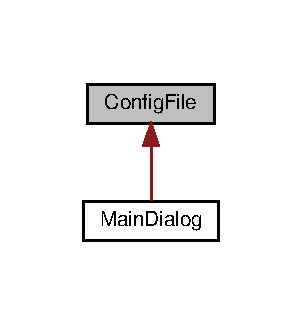
\includegraphics[width=145pt]{classConfigFile__inherit__graph}
\end{center}
\end{figure}
\subsection*{Public Member Functions}
\begin{DoxyCompactItemize}
\item 
\mbox{\Hypertarget{classConfigFile_ab958517fc07a5075b4663e0e46efaed6}\label{classConfigFile_ab958517fc07a5075b4663e0e46efaed6}} 
void \hyperlink{classConfigFile_ab958517fc07a5075b4663e0e46efaed6}{Reset} ()
\begin{DoxyCompactList}\small\item\em deletes the stored parameters \end{DoxyCompactList}\item 
int \hyperlink{classConfigFile_a6dedab9ccb1548b6a0910cee953c0b49}{Get\+Number\+Of\+Variables} ()
\begin{DoxyCompactList}\small\item\em counts the number of stored parameters \end{DoxyCompactList}\item 
bool \hyperlink{classConfigFile_a4395577037347f2af515aaeeded9e727}{Get\+Variable} (std\+::string var\+Name, double \&var\+Value)
\begin{DoxyCompactList}\small\item\em looks if a the parameter is stored and if it is, copies the parameter value \end{DoxyCompactList}\item 
bool \hyperlink{classConfigFile_aa8874c0773572d6853b09414f16472bb}{Is\+Config\+File\+Available} ()
\begin{DoxyCompactList}\small\item\em check if config file is available in folder of the program \end{DoxyCompactList}\item 
\mbox{\Hypertarget{classConfigFile_a60c3135e4354d8f450679130359f5098}\label{classConfigFile_a60c3135e4354d8f450679130359f5098}} 
void \hyperlink{classConfigFile_a60c3135e4354d8f450679130359f5098}{Read\+Config\+File} ()
\begin{DoxyCompactList}\small\item\em reads the config file line by line and stores every parameter \end{DoxyCompactList}\end{DoxyCompactItemize}
\subsection*{Private Member Functions}
\begin{DoxyCompactItemize}
\item 
bool \hyperlink{classConfigFile_a3be9deb6d7f24b7cff36d5746226a440}{Start\+With\+Hash} (std\+::string str)
\begin{DoxyCompactList}\small\item\em check if the string starts with a hash. Leading whitespaces are ignored. \end{DoxyCompactList}\end{DoxyCompactItemize}
\subsection*{Private Attributes}
\begin{DoxyCompactItemize}
\item 
\mbox{\Hypertarget{classConfigFile_a22529d587b96238050d2bf399190cc76}\label{classConfigFile_a22529d587b96238050d2bf399190cc76}} 
const std\+::string \hyperlink{classConfigFile_a22529d587b96238050d2bf399190cc76}{mp\+Config\+File\+Name}
\begin{DoxyCompactList}\small\item\em file name of the config file \end{DoxyCompactList}\item 
\mbox{\Hypertarget{classConfigFile_add6ced4a6aba6f2a67e3be298787c074}\label{classConfigFile_add6ced4a6aba6f2a67e3be298787c074}} 
std\+::list$<$ std\+::tuple$<$ std\+::string, double $>$ $>$ \hyperlink{classConfigFile_add6ced4a6aba6f2a67e3be298787c074}{m\+Variables}
\begin{DoxyCompactList}\small\item\em parameter list. Each list element is a name/value tuple \end{DoxyCompactList}\end{DoxyCompactItemize}


\subsection{Detailed Description}
\begin{DoxyAuthor}{Author}
Matthias Hund 
\end{DoxyAuthor}
\begin{DoxyDate}{Date}
06/06/20 
\end{DoxyDate}


\subsection{Member Function Documentation}
\mbox{\Hypertarget{classConfigFile_a6dedab9ccb1548b6a0910cee953c0b49}\label{classConfigFile_a6dedab9ccb1548b6a0910cee953c0b49}} 
\index{Config\+File@{Config\+File}!Get\+Number\+Of\+Variables@{Get\+Number\+Of\+Variables}}
\index{Get\+Number\+Of\+Variables@{Get\+Number\+Of\+Variables}!Config\+File@{Config\+File}}
\subsubsection{\texorpdfstring{Get\+Number\+Of\+Variables()}{GetNumberOfVariables()}}
{\footnotesize\ttfamily int Config\+File\+::\+Get\+Number\+Of\+Variables (\begin{DoxyParamCaption}{ }\end{DoxyParamCaption})}



counts the number of stored parameters 

\begin{DoxyReturn}{Returns}
number of parameters 
\end{DoxyReturn}
\mbox{\Hypertarget{classConfigFile_a4395577037347f2af515aaeeded9e727}\label{classConfigFile_a4395577037347f2af515aaeeded9e727}} 
\index{Config\+File@{Config\+File}!Get\+Variable@{Get\+Variable}}
\index{Get\+Variable@{Get\+Variable}!Config\+File@{Config\+File}}
\subsubsection{\texorpdfstring{Get\+Variable()}{GetVariable()}}
{\footnotesize\ttfamily bool Config\+File\+::\+Get\+Variable (\begin{DoxyParamCaption}\item[{std\+::string}]{var\+Name,  }\item[{double \&}]{var\+Value }\end{DoxyParamCaption})}



looks if a the parameter is stored and if it is, copies the parameter value 


\begin{DoxyParams}{Parameters}
{\em var\+Name} & name of the parameter searched for \\
\hline
{\em var\+Value} & value of the parameter if it was stored \\
\hline
\end{DoxyParams}
\begin{DoxyReturn}{Returns}
true if the parameter was found, otherwise false 
\end{DoxyReturn}
\mbox{\Hypertarget{classConfigFile_aa8874c0773572d6853b09414f16472bb}\label{classConfigFile_aa8874c0773572d6853b09414f16472bb}} 
\index{Config\+File@{Config\+File}!Is\+Config\+File\+Available@{Is\+Config\+File\+Available}}
\index{Is\+Config\+File\+Available@{Is\+Config\+File\+Available}!Config\+File@{Config\+File}}
\subsubsection{\texorpdfstring{Is\+Config\+File\+Available()}{IsConfigFileAvailable()}}
{\footnotesize\ttfamily bool Config\+File\+::\+Is\+Config\+File\+Available (\begin{DoxyParamCaption}{ }\end{DoxyParamCaption})}



check if config file is available in folder of the program 

\begin{DoxyReturn}{Returns}
true if a config file was found, otherwise false 
\end{DoxyReturn}
\mbox{\Hypertarget{classConfigFile_a3be9deb6d7f24b7cff36d5746226a440}\label{classConfigFile_a3be9deb6d7f24b7cff36d5746226a440}} 
\index{Config\+File@{Config\+File}!Start\+With\+Hash@{Start\+With\+Hash}}
\index{Start\+With\+Hash@{Start\+With\+Hash}!Config\+File@{Config\+File}}
\subsubsection{\texorpdfstring{Start\+With\+Hash()}{StartWithHash()}}
{\footnotesize\ttfamily bool Config\+File\+::\+Start\+With\+Hash (\begin{DoxyParamCaption}\item[{std\+::string}]{str }\end{DoxyParamCaption})\hspace{0.3cm}{\ttfamily [private]}}



check if the string starts with a hash. Leading whitespaces are ignored. 


\begin{DoxyParams}{Parameters}
{\em str} & string to be searched \\
\hline
\end{DoxyParams}
\begin{DoxyReturn}{Returns}
true if the string starts with a hash, otherwise false 
\end{DoxyReturn}


The documentation for this class was generated from the following files\+:\begin{DoxyCompactItemize}
\item 
\hyperlink{ConfigFile_8h}{Config\+File.\+h}\item 
Config\+File.\+cpp\end{DoxyCompactItemize}

\hypertarget{classGlobal}{}\section{Global Class Reference}
\label{classGlobal}\index{Global@{Global}}


{\ttfamily \#include $<$Global.\+h$>$}



Collaboration diagram for Global\+:
\nopagebreak
\begin{figure}[H]
\begin{center}
\leavevmode
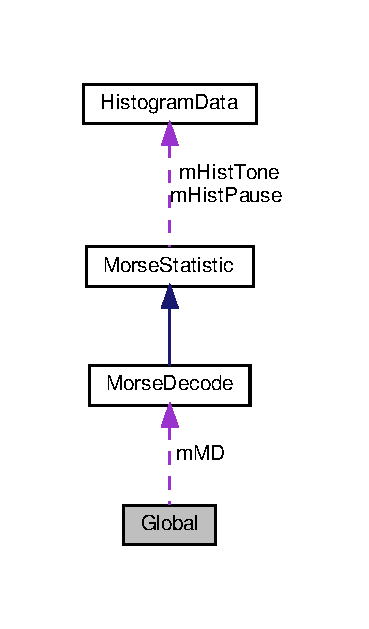
\includegraphics[width=160pt]{classGlobal__coll__graph}
\end{center}
\end{figure}
\subsection*{Static Public Attributes}
\begin{DoxyCompactItemize}
\item 
\mbox{\Hypertarget{classGlobal_acec01a6570ee9e7fcacb53e34f3e07d9}\label{classGlobal_acec01a6570ee9e7fcacb53e34f3e07d9}} 
static \hyperlink{classMorseDecode}{Morse\+Decode} \hyperlink{classGlobal_acec01a6570ee9e7fcacb53e34f3e07d9}{m\+MD}
\begin{DoxyCompactList}\small\item\em \hyperlink{classMorseDecode}{Morse\+Decode} class used to transform the audio signal into a text. \end{DoxyCompactList}\item 
\mbox{\Hypertarget{classGlobal_a381fdad9f072fbfc884f5fd21770c01d}\label{classGlobal_a381fdad9f072fbfc884f5fd21770c01d}} 
static std\+::mutex \hyperlink{classGlobal_a381fdad9f072fbfc884f5fd21770c01d}{m\+M\+D\+Mutex}
\begin{DoxyCompactList}\small\item\em mutex to coordinate access to m\+MD \end{DoxyCompactList}\item 
\mbox{\Hypertarget{classGlobal_a8b6e4fdee334448daa515c479f811c16}\label{classGlobal_a8b6e4fdee334448daa515c479f811c16}} 
static bool \hyperlink{classGlobal_a8b6e4fdee334448daa515c479f811c16}{m\+Stop\+Listen}
\begin{DoxyCompactList}\small\item\em flag to indicate the listen thread that it should terminate \end{DoxyCompactList}\item 
\mbox{\Hypertarget{classGlobal_af3946aac777799a0d5c1df0a7a5abcdb}\label{classGlobal_af3946aac777799a0d5c1df0a7a5abcdb}} 
static std\+::string \hyperlink{classGlobal_af3946aac777799a0d5c1df0a7a5abcdb}{m\+Audio\+Dev}
\begin{DoxyCompactList}\small\item\em name of the audio input device that should be used \end{DoxyCompactList}\end{DoxyCompactItemize}


\subsection{Detailed Description}
\begin{DoxyAuthor}{Author}
Matthias Hund 
\end{DoxyAuthor}
\begin{DoxyDate}{Date}
06/17/20 
\end{DoxyDate}


The documentation for this class was generated from the following files\+:\begin{DoxyCompactItemize}
\item 
\hyperlink{Global_8h}{Global.\+h}\item 
Global.\+cpp\end{DoxyCompactItemize}

\hypertarget{classMainApp}{}\section{Main\+App Class Reference}
\label{classMainApp}\index{Main\+App@{Main\+App}}


{\ttfamily \#include $<$Main.\+h$>$}



Inheritance diagram for Main\+App\+:\nopagebreak
\begin{figure}[H]
\begin{center}
\leavevmode
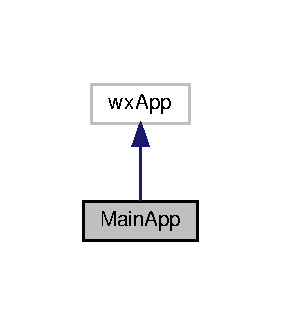
\includegraphics[width=135pt]{classMainApp__inherit__graph}
\end{center}
\end{figure}


Collaboration diagram for Main\+App\+:\nopagebreak
\begin{figure}[H]
\begin{center}
\leavevmode
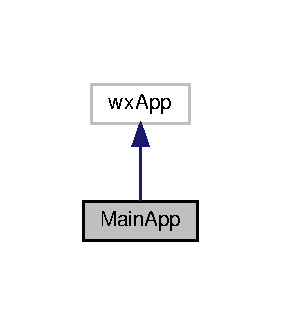
\includegraphics[width=135pt]{classMainApp__coll__graph}
\end{center}
\end{figure}
\subsection*{Public Member Functions}
\begin{DoxyCompactItemize}
\item 
virtual bool \hyperlink{classMainApp_aff3d398e1b61f1016c37d57798f86731}{On\+Init} ()
\begin{DoxyCompactList}\small\item\em application class implementation \end{DoxyCompactList}\end{DoxyCompactItemize}


\subsection{Detailed Description}
\begin{DoxyAuthor}{Author}
Matthias Hund 
\end{DoxyAuthor}
\begin{DoxyDate}{Date}
06/06/20 
\end{DoxyDate}


\subsection{Member Function Documentation}
\mbox{\Hypertarget{classMainApp_aff3d398e1b61f1016c37d57798f86731}\label{classMainApp_aff3d398e1b61f1016c37d57798f86731}} 
\index{Main\+App@{Main\+App}!On\+Init@{On\+Init}}
\index{On\+Init@{On\+Init}!Main\+App@{Main\+App}}
\subsubsection{\texorpdfstring{On\+Init()}{OnInit()}}
{\footnotesize\ttfamily bool Main\+App\+::\+On\+Init (\begin{DoxyParamCaption}{ }\end{DoxyParamCaption})\hspace{0.3cm}{\ttfamily [virtual]}}



application class implementation 

\begin{DoxyReturn}{Returns}
returns always true 
\end{DoxyReturn}


The documentation for this class was generated from the following files\+:\begin{DoxyCompactItemize}
\item 
\hyperlink{Main_8h}{Main.\+h}\item 
Main.\+cpp\end{DoxyCompactItemize}

\hypertarget{classMainDialog}{}\section{Main\+Dialog Class Reference}
\label{classMainDialog}\index{Main\+Dialog@{Main\+Dialog}}


{\ttfamily \#include $<$Main\+Dialog.\+h$>$}



Inheritance diagram for Main\+Dialog\+:\nopagebreak
\begin{figure}[H]
\begin{center}
\leavevmode
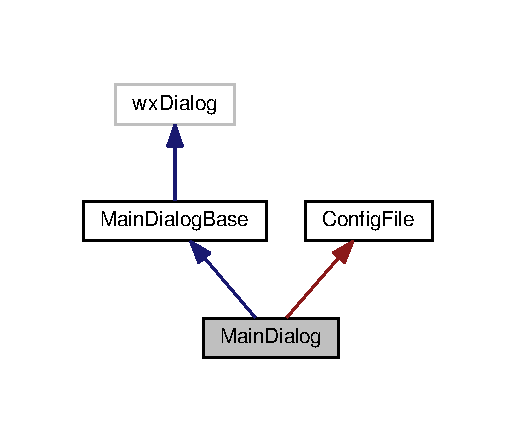
\includegraphics[width=248pt]{classMainDialog__inherit__graph}
\end{center}
\end{figure}


Collaboration diagram for Main\+Dialog\+:\nopagebreak
\begin{figure}[H]
\begin{center}
\leavevmode
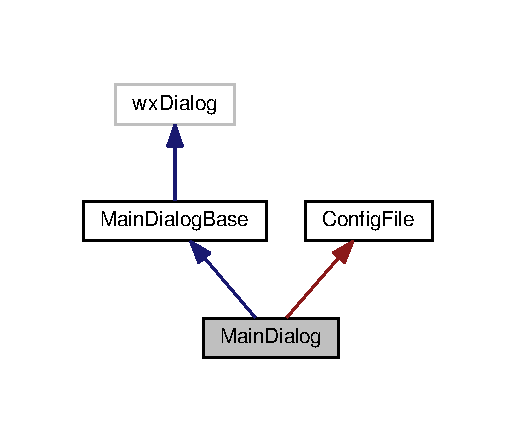
\includegraphics[width=248pt]{classMainDialog__coll__graph}
\end{center}
\end{figure}
\subsection*{Public Member Functions}
\begin{DoxyCompactItemize}
\item 
\hyperlink{classMainDialog_ae4bae8f15a5729712a7fd4effd078063}{Main\+Dialog} (wx\+Window $\ast$parent)
\begin{DoxyCompactList}\small\item\em constructor of the main dialog. Does some setups. \end{DoxyCompactList}\item 
\hyperlink{classMainDialog_a33d8e8327530b31387876b19f6542cc5}{$\sim$\+Main\+Dialog} ()
\begin{DoxyCompactList}\small\item\em destructor of the main dialog, that will stop any processing \end{DoxyCompactList}\end{DoxyCompactItemize}
\subsection*{Protected Member Functions}
\begin{DoxyCompactItemize}
\item 
void \hyperlink{classMainDialog_a17fec54d5486bc4e44052bcef47f3fcc}{On\+Close\+Dialog} (wx\+Close\+Event \&event)
\begin{DoxyCompactList}\small\item\em if the user want to close application destroy it \end{DoxyCompactList}\item 
void \hyperlink{classMainDialog_a505dcb8188eafd19d3fe21b382ec7fe7}{on\+Button\+Stop} (wx\+Command\+Event \&event)
\begin{DoxyCompactList}\small\item\em if \char`\"{}stop\char`\"{} button is pressed finish listen thread and stop update timer \end{DoxyCompactList}\item 
void \hyperlink{classMainDialog_a4feedd725b68a028c72c2227c4c55976}{on\+Button\+Start} (wx\+Command\+Event \&event)
\begin{DoxyCompactList}\small\item\em if \char`\"{}start\char`\"{} button is pressed run listen thread and start timer to update widgets repeatedly \end{DoxyCompactList}\item 
void \hyperlink{classMainDialog_a121d263ec1ae91147a8947dad64b984f}{on\+Clear\+Output\+Txt} (wx\+Command\+Event \&event)
\begin{DoxyCompactList}\small\item\em if \char`\"{}clear\char`\"{} button is pushed, clear the decoded output text of the tect control widget \end{DoxyCompactList}\item 
void \hyperlink{classMainDialog_a562ef211b7cfd5ae24a9f04f41ccb67e}{on\+Timer\+Out} (wx\+Timer\+Event \&event)
\begin{DoxyCompactList}\small\item\em if timer is elapsed, update variables and the widgets int the morse output section \end{DoxyCompactList}\item 
void \hyperlink{classMainDialog_a2b15d3ae06d0b3e1246bcd012f8f758a}{on\+Timer\+Stat} (wx\+Timer\+Event \&event)
\begin{DoxyCompactList}\small\item\em if timer is elapsed, update variables and the widgets int the statistic section \end{DoxyCompactList}\item 
void \hyperlink{classMainDialog_a6c56256388bab3fe16995c722a072d33}{on\+Gain\+Scroll} (wx\+Scroll\+Event \&event)
\begin{DoxyCompactList}\small\item\em if slider is moved change gain by setting a new maximal amplitude \end{DoxyCompactList}\item 
\mbox{\Hypertarget{classMainDialog_afcdc2324728aa4e44b4a8a7e2686cf24}\label{classMainDialog_afcdc2324728aa4e44b4a8a7e2686cf24}} 
void {\bfseries On\+Show\+Histogram} (wx\+Command\+Event \&event)
\item 
\mbox{\Hypertarget{classMainDialog_acc02224a5aa1dd5a8db355dcd6d04a8d}\label{classMainDialog_acc02224a5aa1dd5a8db355dcd6d04a8d}} 
void {\bfseries On\+Close} (wx\+Command\+Event \&event)
\end{DoxyCompactItemize}
\subsection*{Private Member Functions}
\begin{DoxyCompactItemize}
\item 
\mbox{\Hypertarget{classMainDialog_ada04a88fdfc5b3b0921e26f23f7f1fc4}\label{classMainDialog_ada04a88fdfc5b3b0921e26f23f7f1fc4}} 
void \hyperlink{classMainDialog_ada04a88fdfc5b3b0921e26f23f7f1fc4}{Setup\+Morse\+Decode} ()
\begin{DoxyCompactList}\small\item\em read parameter if available and setup the \hyperlink{classMorseDecode}{Morse\+Decode} instance. \end{DoxyCompactList}\item 
\mbox{\Hypertarget{classMainDialog_acd93dbfb870680e4dff510d88f1d3125}\label{classMainDialog_acd93dbfb870680e4dff510d88f1d3125}} 
void {\bfseries Clear\+Widgets} ()
\end{DoxyCompactItemize}
\subsection*{Private Attributes}
\begin{DoxyCompactItemize}
\item 
\mbox{\Hypertarget{classMainDialog_af4537bbf090137035880a13f50cb9789}\label{classMainDialog_af4537bbf090137035880a13f50cb9789}} 
std\+::thread $\ast$ \hyperlink{classMainDialog_af4537bbf090137035880a13f50cb9789}{mp\+Listen\+Thread}
\begin{DoxyCompactList}\small\item\em pointer to the listen thread that process the audio data \end{DoxyCompactList}\item 
\mbox{\Hypertarget{classMainDialog_ae61ec8f7594554de53ccbf6fea4e7493}\label{classMainDialog_ae61ec8f7594554de53ccbf6fea4e7493}} 
std\+::time\+\_\+t \hyperlink{classMainDialog_ae61ec8f7594554de53ccbf6fea4e7493}{m\+Timer\+No\+Receive}
\begin{DoxyCompactList}\small\item\em timestamp used to check if nothing is received \end{DoxyCompactList}\item 
\mbox{\Hypertarget{classMainDialog_a12e6e6ff1f1d3532b607d0ada1e3698d}\label{classMainDialog_a12e6e6ff1f1d3532b607d0ada1e3698d}} 
std\+::time\+\_\+t \hyperlink{classMainDialog_a12e6e6ff1f1d3532b607d0ada1e3698d}{m\+Flush\+Timeout}
\begin{DoxyCompactList}\small\item\em time interval before output is flushed \end{DoxyCompactList}\item 
\mbox{\Hypertarget{classMainDialog_a9abeb88ddd08e9f442ff3be153a8e6c4}\label{classMainDialog_a9abeb88ddd08e9f442ff3be153a8e6c4}} 
unsigned int \hyperlink{classMainDialog_a9abeb88ddd08e9f442ff3be153a8e6c4}{m\+Add\+New\+Line}
\begin{DoxyCompactList}\small\item\em helper variable used to add a new line if nothing is received for a while \end{DoxyCompactList}\end{DoxyCompactItemize}
\subsection*{Additional Inherited Members}


\subsection{Detailed Description}
Implementing \hyperlink{classMainDialogBase}{Main\+Dialog\+Base}

\begin{DoxyAuthor}{Author}
Matthias Hund 
\end{DoxyAuthor}
\begin{DoxyDate}{Date}
06/06/20 
\end{DoxyDate}


\subsection{Constructor \& Destructor Documentation}
\mbox{\Hypertarget{classMainDialog_ae4bae8f15a5729712a7fd4effd078063}\label{classMainDialog_ae4bae8f15a5729712a7fd4effd078063}} 
\index{Main\+Dialog@{Main\+Dialog}!Main\+Dialog@{Main\+Dialog}}
\index{Main\+Dialog@{Main\+Dialog}!Main\+Dialog@{Main\+Dialog}}
\subsubsection{\texorpdfstring{Main\+Dialog()}{MainDialog()}}
{\footnotesize\ttfamily Main\+Dialog\+::\+Main\+Dialog (\begin{DoxyParamCaption}\item[{wx\+Window $\ast$}]{parent }\end{DoxyParamCaption})}



constructor of the main dialog. Does some setups. 

Constructor


\begin{DoxyParams}{Parameters}
{\em parent} & \\
\hline
\end{DoxyParams}
\mbox{\Hypertarget{classMainDialog_a33d8e8327530b31387876b19f6542cc5}\label{classMainDialog_a33d8e8327530b31387876b19f6542cc5}} 
\index{Main\+Dialog@{Main\+Dialog}!````~Main\+Dialog@{$\sim$\+Main\+Dialog}}
\index{````~Main\+Dialog@{$\sim$\+Main\+Dialog}!Main\+Dialog@{Main\+Dialog}}
\subsubsection{\texorpdfstring{$\sim$\+Main\+Dialog()}{~MainDialog()}}
{\footnotesize\ttfamily Main\+Dialog\+::$\sim$\+Main\+Dialog (\begin{DoxyParamCaption}{ }\end{DoxyParamCaption})}



destructor of the main dialog, that will stop any processing 

\begin{DoxyReturn}{Returns}

\end{DoxyReturn}


\subsection{Member Function Documentation}
\mbox{\Hypertarget{classMainDialog_a4feedd725b68a028c72c2227c4c55976}\label{classMainDialog_a4feedd725b68a028c72c2227c4c55976}} 
\index{Main\+Dialog@{Main\+Dialog}!on\+Button\+Start@{on\+Button\+Start}}
\index{on\+Button\+Start@{on\+Button\+Start}!Main\+Dialog@{Main\+Dialog}}
\subsubsection{\texorpdfstring{on\+Button\+Start()}{onButtonStart()}}
{\footnotesize\ttfamily void Main\+Dialog\+::on\+Button\+Start (\begin{DoxyParamCaption}\item[{wx\+Command\+Event \&}]{event }\end{DoxyParamCaption})\hspace{0.3cm}{\ttfamily [protected]}, {\ttfamily [virtual]}}



if \char`\"{}start\char`\"{} button is pressed run listen thread and start timer to update widgets repeatedly 


\begin{DoxyParams}{Parameters}
{\em event} & \\
\hline
\end{DoxyParams}


Reimplemented from \hyperlink{classMainDialogBase}{Main\+Dialog\+Base}.

\mbox{\Hypertarget{classMainDialog_a505dcb8188eafd19d3fe21b382ec7fe7}\label{classMainDialog_a505dcb8188eafd19d3fe21b382ec7fe7}} 
\index{Main\+Dialog@{Main\+Dialog}!on\+Button\+Stop@{on\+Button\+Stop}}
\index{on\+Button\+Stop@{on\+Button\+Stop}!Main\+Dialog@{Main\+Dialog}}
\subsubsection{\texorpdfstring{on\+Button\+Stop()}{onButtonStop()}}
{\footnotesize\ttfamily void Main\+Dialog\+::on\+Button\+Stop (\begin{DoxyParamCaption}\item[{wx\+Command\+Event \&}]{event }\end{DoxyParamCaption})\hspace{0.3cm}{\ttfamily [protected]}, {\ttfamily [virtual]}}



if \char`\"{}stop\char`\"{} button is pressed finish listen thread and stop update timer 


\begin{DoxyParams}{Parameters}
{\em event} & \\
\hline
\end{DoxyParams}


Reimplemented from \hyperlink{classMainDialogBase}{Main\+Dialog\+Base}.

\mbox{\Hypertarget{classMainDialog_a121d263ec1ae91147a8947dad64b984f}\label{classMainDialog_a121d263ec1ae91147a8947dad64b984f}} 
\index{Main\+Dialog@{Main\+Dialog}!on\+Clear\+Output\+Txt@{on\+Clear\+Output\+Txt}}
\index{on\+Clear\+Output\+Txt@{on\+Clear\+Output\+Txt}!Main\+Dialog@{Main\+Dialog}}
\subsubsection{\texorpdfstring{on\+Clear\+Output\+Txt()}{onClearOutputTxt()}}
{\footnotesize\ttfamily void Main\+Dialog\+::on\+Clear\+Output\+Txt (\begin{DoxyParamCaption}\item[{wx\+Command\+Event \&}]{event }\end{DoxyParamCaption})\hspace{0.3cm}{\ttfamily [protected]}, {\ttfamily [virtual]}}



if \char`\"{}clear\char`\"{} button is pushed, clear the decoded output text of the tect control widget 


\begin{DoxyParams}{Parameters}
{\em event} & \\
\hline
\end{DoxyParams}


Reimplemented from \hyperlink{classMainDialogBase}{Main\+Dialog\+Base}.

\mbox{\Hypertarget{classMainDialog_a17fec54d5486bc4e44052bcef47f3fcc}\label{classMainDialog_a17fec54d5486bc4e44052bcef47f3fcc}} 
\index{Main\+Dialog@{Main\+Dialog}!On\+Close\+Dialog@{On\+Close\+Dialog}}
\index{On\+Close\+Dialog@{On\+Close\+Dialog}!Main\+Dialog@{Main\+Dialog}}
\subsubsection{\texorpdfstring{On\+Close\+Dialog()}{OnCloseDialog()}}
{\footnotesize\ttfamily void Main\+Dialog\+::\+On\+Close\+Dialog (\begin{DoxyParamCaption}\item[{wx\+Close\+Event \&}]{event }\end{DoxyParamCaption})\hspace{0.3cm}{\ttfamily [protected]}, {\ttfamily [virtual]}}



if the user want to close application destroy it 


\begin{DoxyParams}{Parameters}
{\em event} & \\
\hline
\end{DoxyParams}


Reimplemented from \hyperlink{classMainDialogBase}{Main\+Dialog\+Base}.

\mbox{\Hypertarget{classMainDialog_a6c56256388bab3fe16995c722a072d33}\label{classMainDialog_a6c56256388bab3fe16995c722a072d33}} 
\index{Main\+Dialog@{Main\+Dialog}!on\+Gain\+Scroll@{on\+Gain\+Scroll}}
\index{on\+Gain\+Scroll@{on\+Gain\+Scroll}!Main\+Dialog@{Main\+Dialog}}
\subsubsection{\texorpdfstring{on\+Gain\+Scroll()}{onGainScroll()}}
{\footnotesize\ttfamily void Main\+Dialog\+::on\+Gain\+Scroll (\begin{DoxyParamCaption}\item[{wx\+Scroll\+Event \&}]{event }\end{DoxyParamCaption})\hspace{0.3cm}{\ttfamily [protected]}, {\ttfamily [virtual]}}



if slider is moved change gain by setting a new maximal amplitude 


\begin{DoxyParams}{Parameters}
{\em event} & \\
\hline
\end{DoxyParams}


Reimplemented from \hyperlink{classMainDialogBase}{Main\+Dialog\+Base}.

\mbox{\Hypertarget{classMainDialog_a562ef211b7cfd5ae24a9f04f41ccb67e}\label{classMainDialog_a562ef211b7cfd5ae24a9f04f41ccb67e}} 
\index{Main\+Dialog@{Main\+Dialog}!on\+Timer\+Out@{on\+Timer\+Out}}
\index{on\+Timer\+Out@{on\+Timer\+Out}!Main\+Dialog@{Main\+Dialog}}
\subsubsection{\texorpdfstring{on\+Timer\+Out()}{onTimerOut()}}
{\footnotesize\ttfamily void Main\+Dialog\+::on\+Timer\+Out (\begin{DoxyParamCaption}\item[{wx\+Timer\+Event \&}]{event }\end{DoxyParamCaption})\hspace{0.3cm}{\ttfamily [protected]}, {\ttfamily [virtual]}}



if timer is elapsed, update variables and the widgets int the morse output section 


\begin{DoxyParams}{Parameters}
{\em event} & \\
\hline
\end{DoxyParams}


Reimplemented from \hyperlink{classMainDialogBase}{Main\+Dialog\+Base}.

\mbox{\Hypertarget{classMainDialog_a2b15d3ae06d0b3e1246bcd012f8f758a}\label{classMainDialog_a2b15d3ae06d0b3e1246bcd012f8f758a}} 
\index{Main\+Dialog@{Main\+Dialog}!on\+Timer\+Stat@{on\+Timer\+Stat}}
\index{on\+Timer\+Stat@{on\+Timer\+Stat}!Main\+Dialog@{Main\+Dialog}}
\subsubsection{\texorpdfstring{on\+Timer\+Stat()}{onTimerStat()}}
{\footnotesize\ttfamily void Main\+Dialog\+::on\+Timer\+Stat (\begin{DoxyParamCaption}\item[{wx\+Timer\+Event \&}]{event }\end{DoxyParamCaption})\hspace{0.3cm}{\ttfamily [protected]}, {\ttfamily [virtual]}}



if timer is elapsed, update variables and the widgets int the statistic section 


\begin{DoxyParams}{Parameters}
{\em event} & \\
\hline
\end{DoxyParams}


Reimplemented from \hyperlink{classMainDialogBase}{Main\+Dialog\+Base}.



The documentation for this class was generated from the following files\+:\begin{DoxyCompactItemize}
\item 
\hyperlink{MainDialog_8h}{Main\+Dialog.\+h}\item 
Main\+Dialog.\+cpp\end{DoxyCompactItemize}

\hypertarget{classMainDialogBase}{}\section{Main\+Dialog\+Base Class Reference}
\label{classMainDialogBase}\index{Main\+Dialog\+Base@{Main\+Dialog\+Base}}


Class \hyperlink{classMainDialogBase}{Main\+Dialog\+Base}.  




{\ttfamily \#include $<$Morse\+G\+U\+I.\+h$>$}



Inheritance diagram for Main\+Dialog\+Base\+:\nopagebreak
\begin{figure}[H]
\begin{center}
\leavevmode
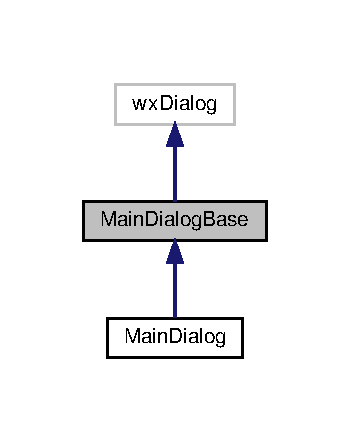
\includegraphics[width=168pt]{classMainDialogBase__inherit__graph}
\end{center}
\end{figure}


Collaboration diagram for Main\+Dialog\+Base\+:\nopagebreak
\begin{figure}[H]
\begin{center}
\leavevmode
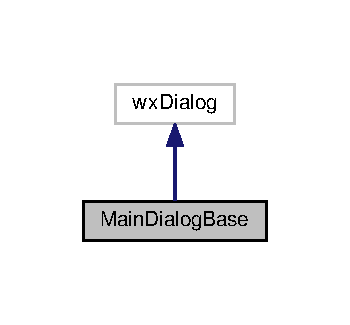
\includegraphics[width=168pt]{classMainDialogBase__coll__graph}
\end{center}
\end{figure}
\subsection*{Public Member Functions}
\begin{DoxyCompactItemize}
\item 
\mbox{\Hypertarget{classMainDialogBase_a5a0347105bfbdf43f0cb282a8ffd3f3f}\label{classMainDialogBase_a5a0347105bfbdf43f0cb282a8ffd3f3f}} 
{\bfseries Main\+Dialog\+Base} (wx\+Window $\ast$parent, wx\+Window\+ID id=wx\+I\+D\+\_\+\+A\+NY, const wx\+String \&title=\+\_\+(\char`\"{}Seventythree\char`\"{}), const wx\+Point \&pos=wx\+Default\+Position, const wx\+Size \&size=wx\+Size(663, 458), long style=wx\+C\+L\+O\+S\+E\+\_\+\+B\+OX$\vert$wx\+D\+E\+F\+A\+U\+L\+T\+\_\+\+D\+I\+A\+L\+O\+G\+\_\+\+S\+T\+Y\+LE$\vert$wx\+R\+E\+S\+I\+Z\+E\+\_\+\+B\+O\+R\+D\+ER)
\end{DoxyCompactItemize}
\subsection*{Protected Member Functions}
\begin{DoxyCompactItemize}
\item 
\mbox{\Hypertarget{classMainDialogBase_a2d753c85ed39df5a546e7a9d5fa45363}\label{classMainDialogBase_a2d753c85ed39df5a546e7a9d5fa45363}} 
virtual void {\bfseries On\+Close\+Dialog} (wx\+Close\+Event \&event)
\item 
\mbox{\Hypertarget{classMainDialogBase_a2904b88a4192bfa3d8a214e122849573}\label{classMainDialogBase_a2904b88a4192bfa3d8a214e122849573}} 
virtual void {\bfseries on\+Clear\+Output\+Txt} (wx\+Command\+Event \&event)
\item 
\mbox{\Hypertarget{classMainDialogBase_a81e778d99d7377020d385182795fca3b}\label{classMainDialogBase_a81e778d99d7377020d385182795fca3b}} 
virtual void {\bfseries on\+Gain\+Scroll} (wx\+Scroll\+Event \&event)
\item 
\mbox{\Hypertarget{classMainDialogBase_a484518dca56c0fca7767652fa01492f6}\label{classMainDialogBase_a484518dca56c0fca7767652fa01492f6}} 
virtual void {\bfseries on\+Button\+Stop} (wx\+Command\+Event \&event)
\item 
\mbox{\Hypertarget{classMainDialogBase_af75b2ee75e323e469c28c2d85dcbb9f8}\label{classMainDialogBase_af75b2ee75e323e469c28c2d85dcbb9f8}} 
virtual void {\bfseries on\+Button\+Start} (wx\+Command\+Event \&event)
\item 
\mbox{\Hypertarget{classMainDialogBase_a9c153c9fe10fa8350d11fb09a0646779}\label{classMainDialogBase_a9c153c9fe10fa8350d11fb09a0646779}} 
virtual void {\bfseries on\+Timer\+Out} (wx\+Timer\+Event \&event)
\item 
\mbox{\Hypertarget{classMainDialogBase_a82bbbaffba00c419a848725e4c05e233}\label{classMainDialogBase_a82bbbaffba00c419a848725e4c05e233}} 
virtual void {\bfseries on\+Timer\+Stat} (wx\+Timer\+Event \&event)
\end{DoxyCompactItemize}
\subsection*{Protected Attributes}
\begin{DoxyCompactItemize}
\item 
\mbox{\Hypertarget{classMainDialogBase_a083d24a490465c25114d9290079eaa69}\label{classMainDialogBase_a083d24a490465c25114d9290079eaa69}} 
wx\+Static\+Text $\ast$ {\bfseries m\+\_\+static\+Text1}
\item 
\mbox{\Hypertarget{classMainDialogBase_a5aae9d4e63f05c524709bceebcb5a454}\label{classMainDialogBase_a5aae9d4e63f05c524709bceebcb5a454}} 
wx\+Static\+Text $\ast$ {\bfseries m\+\_\+static\+Text9}
\item 
\mbox{\Hypertarget{classMainDialogBase_a6fb943aa51729e753c80547e92f8f63b}\label{classMainDialogBase_a6fb943aa51729e753c80547e92f8f63b}} 
wx\+Gauge $\ast$ {\bfseries m\+\_\+gauge\+Buffer\+Level}
\item 
\mbox{\Hypertarget{classMainDialogBase_a76bf1ff83185cc6a6f7ccab275d24d39}\label{classMainDialogBase_a76bf1ff83185cc6a6f7ccab275d24d39}} 
wx\+Static\+Text $\ast$ {\bfseries m\+\_\+static\+Text\+Status}
\item 
\mbox{\Hypertarget{classMainDialogBase_af2234db84ac97ff805b0612c833fa79e}\label{classMainDialogBase_af2234db84ac97ff805b0612c833fa79e}} 
wx\+Gauge $\ast$ {\bfseries m\+\_\+gauge\+Envelope}
\item 
\mbox{\Hypertarget{classMainDialogBase_a7821051e7b2984d479d5ec3270aaedd8}\label{classMainDialogBase_a7821051e7b2984d479d5ec3270aaedd8}} 
wx\+Static\+Text $\ast$ {\bfseries m\+\_\+static\+Text5}
\item 
\mbox{\Hypertarget{classMainDialogBase_aac418ceb04e7af6f7c832637ea2a3290}\label{classMainDialogBase_aac418ceb04e7af6f7c832637ea2a3290}} 
wx\+Text\+Ctrl $\ast$ {\bfseries m\+\_\+text\+Ctrl\+Intervall}
\item 
\mbox{\Hypertarget{classMainDialogBase_a6366324ff9d4ab67aa3b7b1b519a66ba}\label{classMainDialogBase_a6366324ff9d4ab67aa3b7b1b519a66ba}} 
wx\+Static\+Text $\ast$ {\bfseries m\+\_\+static\+Text4}
\item 
\mbox{\Hypertarget{classMainDialogBase_aa195374bab83b180121b2ebd673da7d3}\label{classMainDialogBase_aa195374bab83b180121b2ebd673da7d3}} 
wx\+Gauge $\ast$ {\bfseries m\+\_\+gauge\+Threshold}
\item 
\mbox{\Hypertarget{classMainDialogBase_a87b90a90cb248853aa908201de030bb1}\label{classMainDialogBase_a87b90a90cb248853aa908201de030bb1}} 
wx\+Static\+Text $\ast$ {\bfseries m\+\_\+static\+Text81}
\item 
\mbox{\Hypertarget{classMainDialogBase_afb6736002ba53a31ddeda7ade6c7d406}\label{classMainDialogBase_afb6736002ba53a31ddeda7ade6c7d406}} 
wx\+Text\+Ctrl $\ast$ {\bfseries m\+\_\+text\+Ctrl\+Speed}
\item 
\mbox{\Hypertarget{classMainDialogBase_acc18043f53e8e72d002cd852467f586a}\label{classMainDialogBase_acc18043f53e8e72d002cd852467f586a}} 
wx\+Static\+Text $\ast$ {\bfseries m\+\_\+static\+Text6}
\item 
\mbox{\Hypertarget{classMainDialogBase_ad2b85a60386b17f43e53466a5df7b649}\label{classMainDialogBase_ad2b85a60386b17f43e53466a5df7b649}} 
wx\+Text\+Ctrl $\ast$ {\bfseries m\+\_\+text\+Ctrl\+Sign}
\item 
\mbox{\Hypertarget{classMainDialogBase_a44f011e7af5b7a7952248e0a0bdbb5b9}\label{classMainDialogBase_a44f011e7af5b7a7952248e0a0bdbb5b9}} 
wx\+Static\+Text $\ast$ {\bfseries m\+\_\+static\+Text15}
\item 
\mbox{\Hypertarget{classMainDialogBase_adef50b33f2ea2c95360dd7dc760d101d}\label{classMainDialogBase_adef50b33f2ea2c95360dd7dc760d101d}} 
wx\+Text\+Ctrl $\ast$ {\bfseries m\+\_\+text\+Ctrl\+W\+PM}
\item 
\mbox{\Hypertarget{classMainDialogBase_a9ac83587cc33883db7b9935892758f32}\label{classMainDialogBase_a9ac83587cc33883db7b9935892758f32}} 
wx\+Button $\ast$ {\bfseries m\+\_\+button\+Clear}
\item 
\mbox{\Hypertarget{classMainDialogBase_a948f93ec93099e75918d628cb8f80665}\label{classMainDialogBase_a948f93ec93099e75918d628cb8f80665}} 
wx\+Static\+Line $\ast$ {\bfseries m\+\_\+staticline2}
\item 
\mbox{\Hypertarget{classMainDialogBase_aeab033bd912480736e43d468a4b691db}\label{classMainDialogBase_aeab033bd912480736e43d468a4b691db}} 
wx\+Static\+Text $\ast$ {\bfseries m\+\_\+static\+Text2}
\item 
\mbox{\Hypertarget{classMainDialogBase_a9649f442cae72695a4dfce021648847d}\label{classMainDialogBase_a9649f442cae72695a4dfce021648847d}} 
wx\+Static\+Text $\ast$ {\bfseries m\+\_\+static\+Text16}
\item 
\mbox{\Hypertarget{classMainDialogBase_af25f458706bf3301fdb8462f2411e522}\label{classMainDialogBase_af25f458706bf3301fdb8462f2411e522}} 
wx\+Slider $\ast$ {\bfseries m\+\_\+slider\+Gain}
\item 
\mbox{\Hypertarget{classMainDialogBase_a12bbca489e500c8b47cb23fa22b5c56e}\label{classMainDialogBase_a12bbca489e500c8b47cb23fa22b5c56e}} 
wx\+Choice $\ast$ {\bfseries m\+\_\+choice\+Input}
\item 
\mbox{\Hypertarget{classMainDialogBase_ac0ca25a083c7fbb82a442203ebe2f019}\label{classMainDialogBase_ac0ca25a083c7fbb82a442203ebe2f019}} 
wx\+Button $\ast$ {\bfseries m\+\_\+button\+Stop}
\item 
\mbox{\Hypertarget{classMainDialogBase_a939c6d22ba12d29e6a74b8e4deaea67b}\label{classMainDialogBase_a939c6d22ba12d29e6a74b8e4deaea67b}} 
wx\+Button $\ast$ {\bfseries m\+\_\+button\+Start}
\item 
\mbox{\Hypertarget{classMainDialogBase_a6119a3ccc723601095f5be2bbf2a9d35}\label{classMainDialogBase_a6119a3ccc723601095f5be2bbf2a9d35}} 
wx\+Static\+Line $\ast$ {\bfseries m\+\_\+static\+Line}
\item 
\mbox{\Hypertarget{classMainDialogBase_a952fc9ace8de1bcedefae9459c35077f}\label{classMainDialogBase_a952fc9ace8de1bcedefae9459c35077f}} 
wx\+Static\+Text $\ast$ {\bfseries m\+\_\+static\+Text91}
\item 
\mbox{\Hypertarget{classMainDialogBase_acedfde3dda2fb75928fa994dc1b66578}\label{classMainDialogBase_acedfde3dda2fb75928fa994dc1b66578}} 
wx\+Static\+Text $\ast$ {\bfseries m\+\_\+static\+Text10}
\item 
\mbox{\Hypertarget{classMainDialogBase_ac78c5dbeed7eec2355273c0e32c73680}\label{classMainDialogBase_ac78c5dbeed7eec2355273c0e32c73680}} 
wx\+Text\+Ctrl $\ast$ {\bfseries m\+\_\+text\+Ctrl\+Stat\+Dot}
\item 
\mbox{\Hypertarget{classMainDialogBase_a5b92345a40d83ac94d007394d5a23241}\label{classMainDialogBase_a5b92345a40d83ac94d007394d5a23241}} 
wx\+Static\+Text $\ast$ {\bfseries m\+\_\+static\+Text12}
\item 
\mbox{\Hypertarget{classMainDialogBase_aafffe6b385c1785aee23e661f2ea52e8}\label{classMainDialogBase_aafffe6b385c1785aee23e661f2ea52e8}} 
wx\+Text\+Ctrl $\ast$ {\bfseries m\+\_\+text\+Ctrl\+Stat\+Dash}
\item 
\mbox{\Hypertarget{classMainDialogBase_ab51599583559dc117957539f029f4383}\label{classMainDialogBase_ab51599583559dc117957539f029f4383}} 
wx\+Static\+Text $\ast$ {\bfseries m\+\_\+static\+Text11}
\item 
\mbox{\Hypertarget{classMainDialogBase_a8bd736834a1f6ef8b49134d4d4d11a00}\label{classMainDialogBase_a8bd736834a1f6ef8b49134d4d4d11a00}} 
wx\+Text\+Ctrl $\ast$ {\bfseries m\+\_\+text\+Ctrl\+Stat\+Space}
\item 
\mbox{\Hypertarget{classMainDialogBase_a88c0890537cff8672284776ef1375485}\label{classMainDialogBase_a88c0890537cff8672284776ef1375485}} 
wx\+Static\+Text $\ast$ {\bfseries m\+\_\+static\+Text13}
\item 
\mbox{\Hypertarget{classMainDialogBase_a6cfe514859b1a8a45b7945550e7b3ee6}\label{classMainDialogBase_a6cfe514859b1a8a45b7945550e7b3ee6}} 
wx\+Text\+Ctrl $\ast$ {\bfseries m\+\_\+text\+Ctrl\+Stat\+Ch\+Space}
\item 
\mbox{\Hypertarget{classMainDialogBase_a91d797f7493de12b1072572c8cd01197}\label{classMainDialogBase_a91d797f7493de12b1072572c8cd01197}} 
wx\+Static\+Text $\ast$ {\bfseries m\+\_\+static\+Text14}
\item 
\mbox{\Hypertarget{classMainDialogBase_ad89261c13d806f0de50c40359dcaf292}\label{classMainDialogBase_ad89261c13d806f0de50c40359dcaf292}} 
wx\+Text\+Ctrl $\ast$ {\bfseries m\+\_\+text\+Ctrl\+Stat\+Word\+Space}
\item 
\mbox{\Hypertarget{classMainDialogBase_a638f225b3c0e165f2b40b9fe9ddfee95}\label{classMainDialogBase_a638f225b3c0e165f2b40b9fe9ddfee95}} 
wx\+Static\+Line $\ast$ {\bfseries m\+\_\+staticline3}
\item 
\mbox{\Hypertarget{classMainDialogBase_ac44c9a46fc50a9ad4cd37dbc2235b69e}\label{classMainDialogBase_ac44c9a46fc50a9ad4cd37dbc2235b69e}} 
wx\+Text\+Ctrl $\ast$ {\bfseries m\+\_\+text\+Ctrl\+Output}
\item 
\mbox{\Hypertarget{classMainDialogBase_a9cbe518b2cd7c32fd11e91937cc09062}\label{classMainDialogBase_a9cbe518b2cd7c32fd11e91937cc09062}} 
wx\+Timer {\bfseries m\+\_\+timer\+Out}
\item 
\mbox{\Hypertarget{classMainDialogBase_a8f6aa440def039635fed532a8674dbde}\label{classMainDialogBase_a8f6aa440def039635fed532a8674dbde}} 
wx\+Timer {\bfseries m\+\_\+timer\+Stat}
\end{DoxyCompactItemize}


\subsection{Detailed Description}
Class \hyperlink{classMainDialogBase}{Main\+Dialog\+Base}. 

The documentation for this class was generated from the following files\+:\begin{DoxyCompactItemize}
\item 
Morse\+G\+U\+I.\+h\item 
Morse\+G\+U\+I.\+cpp\end{DoxyCompactItemize}

\hypertarget{classMorseDecode}{}\section{Morse\+Decode Class Reference}
\label{classMorseDecode}\index{Morse\+Decode@{Morse\+Decode}}


The morse decoder class process a audio stream and output morse signals as a text.  




{\ttfamily \#include $<$Morse\+Decode.\+h$>$}



Inheritance diagram for Morse\+Decode\+:\nopagebreak
\begin{figure}[H]
\begin{center}
\leavevmode
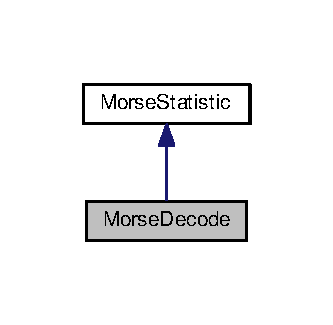
\includegraphics[width=160pt]{classMorseDecode__inherit__graph}
\end{center}
\end{figure}


Collaboration diagram for Morse\+Decode\+:\nopagebreak
\begin{figure}[H]
\begin{center}
\leavevmode
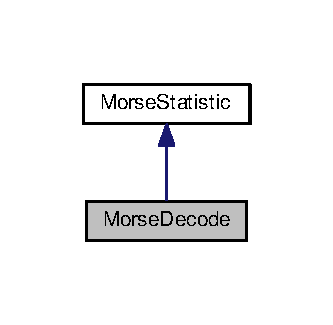
\includegraphics[width=177pt]{classMorseDecode__coll__graph}
\end{center}
\end{figure}
\subsection*{Public Member Functions}
\begin{DoxyCompactItemize}
\item 
\hyperlink{classMorseDecode_a00821fde89334d379f1922fb70ba943b}{Morse\+Decode} (int samples\+Per\+Second, double init\+Dot\+Time=0.\+0655)
\begin{DoxyCompactList}\small\item\em allocates memory for the buffers and initialized variables \end{DoxyCompactList}\item 
\mbox{\Hypertarget{classMorseDecode_ab12ba8f81a417aceb2d2c582ee0e8e07}\label{classMorseDecode_ab12ba8f81a417aceb2d2c582ee0e8e07}} 
\hyperlink{classMorseDecode_ab12ba8f81a417aceb2d2c582ee0e8e07}{$\sim$\+Morse\+Decode} ()
\begin{DoxyCompactList}\small\item\em destructor \end{DoxyCompactList}\item 
\mbox{\Hypertarget{classMorseDecode_ab3f09a593ee52afb44ef555a4c624a68}\label{classMorseDecode_ab3f09a593ee52afb44ef555a4c624a68}} 
void \hyperlink{classMorseDecode_ab3f09a593ee52afb44ef555a4c624a68}{Reset} ()
\begin{DoxyCompactList}\small\item\em reset all variables to default values \end{DoxyCompactList}\item 
const char $\ast$ \hyperlink{classMorseDecode_a9db5d2a826a6795f8a18cf123604d5a9}{Process} (double signal)
\begin{DoxyCompactList}\small\item\em process a new value of the audio input stream nad return characters that are morsed \end{DoxyCompactList}\item 
int \hyperlink{classMorseDecode_a04e9d8784d2e7eec8f725a6e65344839}{Get\+Text} (char $\ast$str, int length)
\begin{DoxyCompactList}\small\item\em copy the recived text from temperary text buffer and reset the buffer \end{DoxyCompactList}\item 
const char $\ast$ \hyperlink{classMorseDecode_a1d3c6ce0ee7c17c55e6ca102a4a6049a}{Get\+Character} (Morse\+::\+Morse\+Sign sign)
\begin{DoxyCompactList}\small\item\em Get a character from a stream of morse signs. The morse signs are collected util a new character begins. The character is looked up if all morse signs of it are recived. \end{DoxyCompactList}\item 
double \hyperlink{classMorseDecode_a610be58591f00c28eb624f062115ce82}{Get\+Amplitude} ()
\begin{DoxyCompactList}\small\item\em access function to the normilzed amplitude \end{DoxyCompactList}\item 
double \hyperlink{classMorseDecode_adc01798960f0f74071eaac3516a4b523}{Get\+Envelope} ()
\begin{DoxyCompactList}\small\item\em access function to the audio signal envelope \end{DoxyCompactList}\item 
double \hyperlink{classMorseDecode_a293ca5977883ebbd4266827491ddeae9}{Get\+Threshold} ()
\begin{DoxyCompactList}\small\item\em access to the threshold value the envelope is compared with \end{DoxyCompactList}\item 
Morse\+::\+Edge\+State \hyperlink{classMorseDecode_a92f19fd07b401876cf132f5f134f2788}{Get\+Edge} ()
\begin{DoxyCompactList}\small\item\em access to the edge state that was detected \end{DoxyCompactList}\item 
double \hyperlink{classMorseDecode_acdc50282bee5f2893d3aeb1210b47ca7}{Get\+Time\+Intervall} ()
\begin{DoxyCompactList}\small\item\em access to the time intervall between the last two edge events \end{DoxyCompactList}\item 
Morse\+::\+Morse\+Sign \hyperlink{classMorseDecode_aae2b17a7fc829a84f2cbc2c9a1577a18}{Get\+Sign} ()
\begin{DoxyCompactList}\small\item\em access to the detected morse sign \end{DoxyCompactList}\item 
Morse\+::\+Morse\+Sign \hyperlink{classMorseDecode_a6986b35715ebadf7a1264e1667c0e253}{Get\+Relevant\+Sign} ()
\begin{DoxyCompactList}\small\item\em return the last relevant morse sign \end{DoxyCompactList}\item 
double \hyperlink{classMorseDecode_a377a7a2c31260c045d472adc96662b85}{Get\+Dot\+Time} ()
\begin{DoxyCompactList}\small\item\em access to the time that was determined for the duration of the morse signe dot \end{DoxyCompactList}\item 
int \hyperlink{classMorseDecode_a716a68423027190d97a59f74aba2f8b3}{Get\+Fill\+Level} ()
\begin{DoxyCompactList}\small\item\em returns the number of elements currently stored in the edge event buffer \end{DoxyCompactList}\item 
int \hyperlink{classMorseDecode_a2827ff2cfbdf56c76154c1d471a0aca5}{Get\+Audio\+In\+Sample\+Rate} ()
\begin{DoxyCompactList}\small\item\em returns the sample rate of the audio input stream \end{DoxyCompactList}\item 
void \hyperlink{classMorseDecode_a34df828f9599e4185b2b0f2999e355b2}{Set\+Audio\+In\+Sample\+Rate} (int rate)
\begin{DoxyCompactList}\small\item\em set the samples per seconds of the audio input stream \end{DoxyCompactList}\item 
void \hyperlink{classMorseDecode_a1b09ba48ee9ae8c7de75e2b4dbb0fdab}{Set\+Max\+Amplitude} (double max\+Amplitude)
\begin{DoxyCompactList}\small\item\em set the maximal amplitude of the audio signal that is passed to \hyperlink{classMorseDecode_a9db5d2a826a6795f8a18cf123604d5a9}{Process()} \end{DoxyCompactList}\item 
void \hyperlink{classMorseDecode_a71b04d87d48e3eb062068bda7fda6ea9}{Set\+Auto\+Threshold\+Factor} (double factor)
\begin{DoxyCompactList}\small\item\em set the target factor of the threshold compared to the maximal envelope \end{DoxyCompactList}\item 
void \hyperlink{classMorseDecode_a5607e1880a8a477af4e5ae5918463971}{Set\+Min\+Threshold} (double min\+Threshold)
\begin{DoxyCompactList}\small\item\em set the minimal value of the threshold \end{DoxyCompactList}\item 
void \hyperlink{classMorseDecode_a7ac2abe729dcd3cce8d53636e6a8c5b2}{Set\+Dot\+Time\+Lower\+Limit} (double lower\+Limit)
\begin{DoxyCompactList}\small\item\em set the lower limit of dot duration \end{DoxyCompactList}\item 
void \hyperlink{classMorseDecode_af73b94d8c654642982a38f5aa0a70beb}{Set\+Dot\+Time\+Upper\+Limit} (double upper\+Limit)
\begin{DoxyCompactList}\small\item\em set the upper limit of dot duration \end{DoxyCompactList}\item 
void \hyperlink{classMorseDecode_a95efbd76c6d03f97868e2e54b5c305cb}{Set\+Stable\+Dot\+Time\+Inaccuracy} (double max\+Inaccuracy)
\begin{DoxyCompactList}\small\item\em set the maximal inaccuracy that is tollerated to esteem dot time as stable \end{DoxyCompactList}\item 
void \hyperlink{classMorseDecode_a2b91a464dd74787aeba96e538ab167ee}{Set\+Max\+Morse\+Signs\+Per\+Char} (uint8\+\_\+t max\+Signs)
\begin{DoxyCompactList}\small\item\em set the maximal number of morse signs a character can have \end{DoxyCompactList}\item 
void \hyperlink{classMorseDecode_a2f5a27e26aa17b37f54fa5353ac02af8}{Set\+Debounce\+Bounce\+Time} (double bounce\+Time)
\begin{DoxyCompactList}\small\item\em set the bounce time \end{DoxyCompactList}\item 
void \hyperlink{classMorseDecode_ac85b7ab4f9e29a9ccb489df2d3501840}{Set\+Low\+Pass\+Decay\+Rate} (double low\+Pass\+Decay\+Rate)
\begin{DoxyCompactList}\small\item\em set the low pass decay rate \end{DoxyCompactList}\item 
void \hyperlink{classMorseDecode_a6fd8645b7dda1b84af1941a9f5d155af}{Set\+Auto\+Threshold\+Decay\+Rate} (double auto\+Threshold\+Decay\+Rate)
\begin{DoxyCompactList}\small\item\em set the decay rate of the threshold \end{DoxyCompactList}\item 
void \hyperlink{classMorseDecode_ae6da2e624d2ce1c8cbc1324757271627}{Set\+Ave\+Time\+Buffer\+Length} (uint8\+\_\+t ave\+Time\+Buffer\+Length)
\begin{DoxyCompactList}\small\item\em set the length of the average time \end{DoxyCompactList}\item 
void \hyperlink{classMorseDecode_ac3d5e669b19c651d522b7f271da53640}{Set\+Short\+Time\+Buffer\+Length} (uint8\+\_\+t shrt\+Time\+Buffer\+Length)
\begin{DoxyCompactList}\small\item\em set the length of the shortest time buffer \end{DoxyCompactList}\item 
void \hyperlink{classMorseDecode_aaaf7bfea0a9bcf523685da983b2bec20}{Set\+Stable\+Dot\+Time\+Buffer\+Length} (uint8\+\_\+t stable\+Dot\+Time\+Buffer\+Length)
\begin{DoxyCompactList}\small\item\em set the length of the stable dot time buffer \end{DoxyCompactList}\item 
void \hyperlink{classMorseDecode_a854d3dd4a5ec6a6a989543baa4d859c3}{Set\+Edge\+Event\+Buffer\+Length} (uint8\+\_\+t edge\+Event\+Buffer\+Length)
\begin{DoxyCompactList}\small\item\em set length of the edge event buffer \end{DoxyCompactList}\item 
void \hyperlink{classMorseDecode_a53d7aedff642bc7b0111454bf32678fb}{Set\+Text\+Buffer\+Length} (int text\+Buffer\+Length)
\begin{DoxyCompactList}\small\item\em set text message buffer length \end{DoxyCompactList}\item 
void \hyperlink{classMorseDecode_ab83ed381b8126b2fc50d9268abb1c30c}{Set\+Max\+Memory\+Consumption} (int max\+Memory)
\begin{DoxyCompactList}\small\item\em set the amount of memory that should not exceeded \end{DoxyCompactList}\item 
bool \hyperlink{classMorseDecode_a51cac4ec93e72a092348d09f21bc88c9}{Is\+Memory\+Consumtion\+Exceeded} ()
\begin{DoxyCompactList}\small\item\em checkes if memory limit was exceeded \end{DoxyCompactList}\end{DoxyCompactItemize}
\subsection*{Static Public Member Functions}
\begin{DoxyCompactItemize}
\item 
static const char $\ast$ \hyperlink{classMorseDecode_a30edafb7494cc578cf13ec8d27eebcd9}{Get\+Sign\+Str} (Morse\+::\+Morse\+Sign)
\begin{DoxyCompactList}\small\item\em return a label string for a numeriacal value of the Morse\+Sign enum \end{DoxyCompactList}\end{DoxyCompactItemize}
\subsection*{Private Types}
\begin{DoxyCompactItemize}
\item 
enum \hyperlink{classMorseDecode_abe155104534fe272d25da5eb19b317bd}{Signal\+State} \{ {\bfseries U\+N\+K\+O\+WN}, 
{\bfseries L\+OW}, 
{\bfseries H\+I\+GH}
 \}
\end{DoxyCompactItemize}
\subsection*{Private Member Functions}
\begin{DoxyCompactItemize}
\item 
double \hyperlink{classMorseDecode_afbe9abff356a2889ad38e252c2726d07}{Normalized\+Amplitude} (double signal)
\begin{DoxyCompactList}\small\item\em normalize the signal regarding m\+Max\+Amplitude and takes compute the absoulut value \end{DoxyCompactList}\item 
double \hyperlink{classMorseDecode_a04527008e5818221448f082ec516928c}{Lowpass} (double new\+Sample)
\begin{DoxyCompactList}\small\item\em low pass filter for the normalized amplitude to get the envelope of the signal \end{DoxyCompactList}\item 
double \hyperlink{classMorseDecode_af21aeb2136d254ee6fb0139c25dd5d9a}{Automatic\+Threshold} (double envelope)
\begin{DoxyCompactList}\small\item\em Determines a threshold that is about half of the tone amplitude. The threshold is lowered with time and increased if the envelope is more than twice the threshold. \end{DoxyCompactList}\item 
Morse\+::\+Edge\+State \hyperlink{classMorseDecode_a64943543f9a4f2d7a567a59239563adf}{Edge\+Trigger} (double input, double threshold)
\begin{DoxyCompactList}\small\item\em simple edge trigger \end{DoxyCompactList}\item 
Morse\+::\+Edge\+State \hyperlink{classMorseDecode_af7e53eff848faf9e57bb7ae660f2911b}{Debounce} (Morse\+::\+Edge\+State state)
\begin{DoxyCompactList}\small\item\em Debounce the edge state to avoid misinterpretation. The new edge state is stored for some time (lockout time) in a F\+I\+FO buffer. The number of R\+I\+S\+I\+NG and F\+A\+L\+L\+I\+NG states is counted if the element at the F\+I\+FO end is not N\+O\+NE. The state with the most counts is returned and the F\+I\+FO reseted. Note\+: Normaly only one not N\+O\+NE state should be in the buffer at a time. \end{DoxyCompactList}\item 
double \hyperlink{classMorseDecode_a90f76d35c56413f35f59fa88e4c0a95c}{Time\+Gap} (Morse\+::\+Edge\+State state)
\begin{DoxyCompactList}\small\item\em count time between two edge events (not N\+O\+NE states) \end{DoxyCompactList}\item 
double \hyperlink{classMorseDecode_a5a23bce21e6da60ae14a657096cd1e00}{Distinction\+Level} (double l\+Level, double h\+Level)
\begin{DoxyCompactList}\small\item\em determines a distinction level between two time spaces \end{DoxyCompactList}\item 
int \hyperlink{classMorseDecode_ad1f577a49ff5d8f4face188dba8966c7}{Round\+Time} (double time\+Ratio)
\begin{DoxyCompactList}\small\item\em round the time\+Ratio to a integer to compensate impropper timing and simplify further processing \end{DoxyCompactList}\item 
double \hyperlink{classMorseDecode_a40976ef94b368d713808e26cefd2ea60}{Time\+Average} (double new\+Time)
\begin{DoxyCompactList}\small\item\em moving average filter for the dot time \end{DoxyCompactList}\item 
double \hyperlink{classMorseDecode_afd5655c1ea13e9ea09bdc25ef9d0bece}{Time\+Shortest} (double new\+Time)
\begin{DoxyCompactList}\small\item\em deterimes shortest time in a intervall \end{DoxyCompactList}\item 
double \hyperlink{classMorseDecode_ae7a9b7844ed145918d91b6ec7337d7c2}{Detect\+Dot\+Time} (double period)
\begin{DoxyCompactList}\small\item\em Determines the dot time. The shorteste time period that appered in the recent past is determined and average filtered. The dot time is limited to a reasonable range. \end{DoxyCompactList}\item 
Morse\+::\+Morse\+Sign \hyperlink{classMorseDecode_aff88997ef0a7621027bab01be18473a0}{Get\+Morse\+Sign} (double dot\+Time, Morse\+::\+Edge\+State edge, double period)
\begin{DoxyCompactList}\small\item\em find the morse sign that fit best \end{DoxyCompactList}\item 
bool \hyperlink{classMorseDecode_af3dc30a7ec25c0eaba9c3e4c08029939}{Is\+Dot\+Time\+Stable} (double dot\+Time)
\begin{DoxyCompactList}\small\item\em checks if dot time varies only a little \end{DoxyCompactList}\item 
Morse\+::\+Morse\+Sign \hyperlink{classMorseDecode_ad02e7621b4c4e8a5b766dc4f4f31fa05}{Edge\+Event} (Morse\+::\+Edge\+State edge, double period)
\begin{DoxyCompactList}\small\item\em Saves edge state and time period in a buffer and calls \hyperlink{classMorseDecode_aff88997ef0a7621027bab01be18473a0}{Get\+Morse\+Sign()} to get the a Morse sign if dot time is stable. \end{DoxyCompactList}\item 
int \hyperlink{classMorseDecode_a36af09ea953ef87950f654fcf0179294}{Get\+Index} (const uint16\+\_\+t sequence, const uint16\+\_\+t $\ast$sign\+Sequences, uint32\+\_\+t n\+Sequences)
\begin{DoxyCompactList}\small\item\em find array index of a dot/dash sequence \end{DoxyCompactList}\item 
const char $\ast$ \hyperlink{classMorseDecode_a3ff969902811aa7eefbccb027d0cbcda}{Decode\+Character} (uint16\+\_\+t sign\+Buffer, int n\+Signs)
\begin{DoxyCompactList}\small\item\em lookup the character that correspond to a dot/dash sequence \end{DoxyCompactList}\item 
void \hyperlink{classMorseDecode_a9e189d9682a7291f7fc86eb6b86d817d}{Append\+To\+Txt\+Buffer} (const char $\ast$character)
\begin{DoxyCompactList}\small\item\em append a character to the text buffer that stores the decoded text temporary \end{DoxyCompactList}\item 
bool \hyperlink{classMorseDecode_a3d3db86f34bbc8524b3b26e439bcb219}{Is\+Memory\+Limit\+Reached} (int num\+Elmt\+Deleted, int num\+Elmt\+New, int Sizeof\+Elmt)
\begin{DoxyCompactList}\small\item\em helper function that calculates the memory consumption if buffer would be changed \end{DoxyCompactList}\item 
\mbox{\Hypertarget{classMorseDecode_a25c9323b16fe14681b05a8ff78bc3a21}\label{classMorseDecode_a25c9323b16fe14681b05a8ff78bc3a21}} 
void \hyperlink{classMorseDecode_a25c9323b16fe14681b05a8ff78bc3a21}{Free\+Memory} ()
\begin{DoxyCompactList}\small\item\em free the memory \end{DoxyCompactList}\end{DoxyCompactItemize}
\subsection*{Private Attributes}
\begin{DoxyCompactItemize}
\item 
\mbox{\Hypertarget{classMorseDecode_acc486b544f75239a0fe7475d83f16364}\label{classMorseDecode_acc486b544f75239a0fe7475d83f16364}} 
double \hyperlink{classMorseDecode_acc486b544f75239a0fe7475d83f16364}{m\+Amplitude}
\begin{DoxyCompactList}\small\item\em nomalized amplitude \end{DoxyCompactList}\item 
\mbox{\Hypertarget{classMorseDecode_a6964d13d62429d00154b29296f6f57f4}\label{classMorseDecode_a6964d13d62429d00154b29296f6f57f4}} 
double \hyperlink{classMorseDecode_a6964d13d62429d00154b29296f6f57f4}{m\+Envelope}
\begin{DoxyCompactList}\small\item\em envelope of the audio signal \end{DoxyCompactList}\item 
\mbox{\Hypertarget{classMorseDecode_a581a4a2c6ecb87ff4143e158fb886010}\label{classMorseDecode_a581a4a2c6ecb87ff4143e158fb886010}} 
double \hyperlink{classMorseDecode_a581a4a2c6ecb87ff4143e158fb886010}{m\+Threshold}
\begin{DoxyCompactList}\small\item\em threshold the envelope is compared with \end{DoxyCompactList}\item 
\mbox{\Hypertarget{classMorseDecode_a3c55b5406edefe099d97168de64b7d16}\label{classMorseDecode_a3c55b5406edefe099d97168de64b7d16}} 
Morse\+::\+Edge\+State \hyperlink{classMorseDecode_a3c55b5406edefe099d97168de64b7d16}{m\+Edge}
\begin{DoxyCompactList}\small\item\em current trigger state that was detected \end{DoxyCompactList}\item 
\mbox{\Hypertarget{classMorseDecode_af3067dd9f74a50291fec57eef3852b32}\label{classMorseDecode_af3067dd9f74a50291fec57eef3852b32}} 
double \hyperlink{classMorseDecode_af3067dd9f74a50291fec57eef3852b32}{m\+Dt}
\begin{DoxyCompactList}\small\item\em time intervall between last two trigger events \end{DoxyCompactList}\item 
\mbox{\Hypertarget{classMorseDecode_a7f7235efc28159b04c81f58bbec2d0d8}\label{classMorseDecode_a7f7235efc28159b04c81f58bbec2d0d8}} 
Morse\+::\+Morse\+Sign \hyperlink{classMorseDecode_a7f7235efc28159b04c81f58bbec2d0d8}{m\+Sign}
\begin{DoxyCompactList}\small\item\em current morse sign \end{DoxyCompactList}\item 
\mbox{\Hypertarget{classMorseDecode_a73f8859eb0c298eb3c1ab202515c7d0d}\label{classMorseDecode_a73f8859eb0c298eb3c1ab202515c7d0d}} 
Morse\+::\+Morse\+Sign \hyperlink{classMorseDecode_a73f8859eb0c298eb3c1ab202515c7d0d}{m\+Relevant\+Sign}
\begin{DoxyCompactList}\small\item\em store a subset of morse signs, e.\+g. not N\+O\+\_\+\+S\+I\+GN \end{DoxyCompactList}\item 
\mbox{\Hypertarget{classMorseDecode_ab249932bd3cd5a80148985b4739b4bd3}\label{classMorseDecode_ab249932bd3cd5a80148985b4739b4bd3}} 
const char $\ast$ \hyperlink{classMorseDecode_ab249932bd3cd5a80148985b4739b4bd3}{m\+Character}
\begin{DoxyCompactList}\small\item\em last character that was detected \end{DoxyCompactList}\item 
\mbox{\Hypertarget{classMorseDecode_a7de8fb071377853000c9b70ee4b6af9e}\label{classMorseDecode_a7de8fb071377853000c9b70ee4b6af9e}} 
int \hyperlink{classMorseDecode_a7de8fb071377853000c9b70ee4b6af9e}{m\+Samples\+Per\+Second}
\begin{DoxyCompactList}\small\item\em sample rate of the audio stream \end{DoxyCompactList}\item 
\mbox{\Hypertarget{classMorseDecode_acacba823317f140412f46653c2917f56}\label{classMorseDecode_acacba823317f140412f46653c2917f56}} 
double \hyperlink{classMorseDecode_acacba823317f140412f46653c2917f56}{m\+Max\+Amplitude}
\begin{DoxyCompactList}\small\item\em maximal amplitude of the audio stream \end{DoxyCompactList}\item 
\mbox{\Hypertarget{classMorseDecode_a93f880a0bbef2a497a971cdec0162a24}\label{classMorseDecode_a93f880a0bbef2a497a971cdec0162a24}} 
double \hyperlink{classMorseDecode_a93f880a0bbef2a497a971cdec0162a24}{m\+Debounce\+Bounce\+Time}
\begin{DoxyCompactList}\small\item\em lockout time of the debounce function in sceonds \end{DoxyCompactList}\item 
\mbox{\Hypertarget{classMorseDecode_a5320f2da57d9b182e67cf9efcefa5568}\label{classMorseDecode_a5320f2da57d9b182e67cf9efcefa5568}} 
Morse\+::\+Edge\+State $\ast$ \hyperlink{classMorseDecode_a5320f2da57d9b182e67cf9efcefa5568}{m\+Debounce\+Buffer}
\begin{DoxyCompactList}\small\item\em F\+I\+FO buffer to debounce the trigger state. \end{DoxyCompactList}\item 
\mbox{\Hypertarget{classMorseDecode_ab7f82b40e054a0e858343cd63c7104e0}\label{classMorseDecode_ab7f82b40e054a0e858343cd63c7104e0}} 
int \hyperlink{classMorseDecode_ab7f82b40e054a0e858343cd63c7104e0}{m\+Debounce\+Buffer\+Length}
\begin{DoxyCompactList}\small\item\em length of the F\+I\+FO debounce buffer \end{DoxyCompactList}\item 
\mbox{\Hypertarget{classMorseDecode_a4cbeac471ba8131720e2d5e30b9cfdec}\label{classMorseDecode_a4cbeac471ba8131720e2d5e30b9cfdec}} 
int \hyperlink{classMorseDecode_a4cbeac471ba8131720e2d5e30b9cfdec}{m\+Debounc\+Buffer\+Idx\+Front}
\begin{DoxyCompactList}\small\item\em saves the las signal state to determine a if rising or falling edge \end{DoxyCompactList}\item 
\mbox{\Hypertarget{classMorseDecode_a07d5aff46940b30fc177435ad9f58084}\label{classMorseDecode_a07d5aff46940b30fc177435ad9f58084}} 
int \hyperlink{classMorseDecode_a07d5aff46940b30fc177435ad9f58084}{m\+Debounc\+Buffer\+Idx\+End}
\begin{DoxyCompactList}\small\item\em saves the las signal state to determine a if rising or falling edge \end{DoxyCompactList}\item 
\mbox{\Hypertarget{classMorseDecode_ab1bce8b0b5f6e86546915564a115394e}\label{classMorseDecode_ab1bce8b0b5f6e86546915564a115394e}} 
double \hyperlink{classMorseDecode_ab1bce8b0b5f6e86546915564a115394e}{m\+Low\+Pass\+Decay\+Rate}
\begin{DoxyCompactList}\small\item\em decay rate (1/time constant) of the low pass filter in Hz \end{DoxyCompactList}\item 
\mbox{\Hypertarget{classMorseDecode_a863b8dfbb16d6017fa41ca4aba30e4e5}\label{classMorseDecode_a863b8dfbb16d6017fa41ca4aba30e4e5}} 
int \hyperlink{classMorseDecode_a863b8dfbb16d6017fa41ca4aba30e4e5}{m\+Low\+Pass\+Filter\+Length}
\begin{DoxyCompactList}\small\item\em length of the low pass filter \end{DoxyCompactList}\item 
\mbox{\Hypertarget{classMorseDecode_a3f07851804bb8a61d51e26c02f2e175d}\label{classMorseDecode_a3f07851804bb8a61d51e26c02f2e175d}} 
int \hyperlink{classMorseDecode_a3f07851804bb8a61d51e26c02f2e175d}{m\+Low\+Passf\+Index}
\begin{DoxyCompactList}\small\item\em current index of the low pass filter \end{DoxyCompactList}\item 
\mbox{\Hypertarget{classMorseDecode_ac9eb40f85100d73cecd36164ac5344e3}\label{classMorseDecode_ac9eb40f85100d73cecd36164ac5344e3}} 
double $\ast$ \hyperlink{classMorseDecode_ac9eb40f85100d73cecd36164ac5344e3}{m\+Low\+Pass\+Filter\+Buffer}
\begin{DoxyCompactList}\small\item\em buffer to store filter elements \end{DoxyCompactList}\item 
\mbox{\Hypertarget{classMorseDecode_acd234ffaeaf179f298be96d841e6e93e}\label{classMorseDecode_acd234ffaeaf179f298be96d841e6e93e}} 
double \hyperlink{classMorseDecode_acd234ffaeaf179f298be96d841e6e93e}{m\+Lowpass\+Damping}
\begin{DoxyCompactList}\small\item\em damping value each filter element is multiplied with \end{DoxyCompactList}\item 
\mbox{\Hypertarget{classMorseDecode_a35d6adcb3d15cc6b5828c50ed8c9e55b}\label{classMorseDecode_a35d6adcb3d15cc6b5828c50ed8c9e55b}} 
double \hyperlink{classMorseDecode_a35d6adcb3d15cc6b5828c50ed8c9e55b}{m\+Auto\+Threshold\+Decay\+Rate}
\begin{DoxyCompactList}\small\item\em decay rate (1/time constant) of the threshold damping in Hz \end{DoxyCompactList}\item 
\mbox{\Hypertarget{classMorseDecode_a7d3a73d4ac6f0a4facf3f4f1bdd018d0}\label{classMorseDecode_a7d3a73d4ac6f0a4facf3f4f1bdd018d0}} 
double \hyperlink{classMorseDecode_a7d3a73d4ac6f0a4facf3f4f1bdd018d0}{m\+Auto\+Threshold\+Damping}
\begin{DoxyCompactList}\small\item\em damping value each filter element is multiplied with \end{DoxyCompactList}\item 
\mbox{\Hypertarget{classMorseDecode_a0114f518eb79cc9d0bf92c62ba7745e5}\label{classMorseDecode_a0114f518eb79cc9d0bf92c62ba7745e5}} 
double \hyperlink{classMorseDecode_a0114f518eb79cc9d0bf92c62ba7745e5}{m\+Auto\+Threshold\+Min\+Threshold}
\begin{DoxyCompactList}\small\item\em lower limit for the threshold \end{DoxyCompactList}\item 
\mbox{\Hypertarget{classMorseDecode_a5554fd16e578137d3766b6d8760a8f44}\label{classMorseDecode_a5554fd16e578137d3766b6d8760a8f44}} 
double \hyperlink{classMorseDecode_a5554fd16e578137d3766b6d8760a8f44}{m\+Auto\+Threshold\+Factor}
\begin{DoxyCompactList}\small\item\em target factor of the threshold/max(envelope) ratio \end{DoxyCompactList}\item 
\mbox{\Hypertarget{classMorseDecode_af36a0cb450ba6d7080889501dae9359d}\label{classMorseDecode_af36a0cb450ba6d7080889501dae9359d}} 
\hyperlink{classMorseDecode_abe155104534fe272d25da5eb19b317bd}{Signal\+State} \hyperlink{classMorseDecode_af36a0cb450ba6d7080889501dae9359d}{m\+Edge\+Trigger\+Last\+State}
\begin{DoxyCompactList}\small\item\em saves the las signal state to determine a if rising or falling edge \end{DoxyCompactList}\item 
\mbox{\Hypertarget{classMorseDecode_af35e1f28d8f1a5bb8bbb508d74d85cf0}\label{classMorseDecode_af35e1f28d8f1a5bb8bbb508d74d85cf0}} 
unsigned int \hyperlink{classMorseDecode_af35e1f28d8f1a5bb8bbb508d74d85cf0}{m\+Timer\+Digital\+Time}
\begin{DoxyCompactList}\small\item\em timer to count time between to signal states \end{DoxyCompactList}\item 
\mbox{\Hypertarget{classMorseDecode_a73d327af4ea9514602ea336afa8a6e71}\label{classMorseDecode_a73d327af4ea9514602ea336afa8a6e71}} 
unsigned int \hyperlink{classMorseDecode_a73d327af4ea9514602ea336afa8a6e71}{m\+Timer\+Start\+Time}
\begin{DoxyCompactList}\small\item\em start time of the timer \end{DoxyCompactList}\item 
\mbox{\Hypertarget{classMorseDecode_a55c259a7cffa248023b531e0b9be5fe9}\label{classMorseDecode_a55c259a7cffa248023b531e0b9be5fe9}} 
const double \hyperlink{classMorseDecode_a55c259a7cffa248023b531e0b9be5fe9}{m\+Round\+Time\+Level} \mbox{[}4\mbox{]}
\begin{DoxyCompactList}\small\item\em integer values for the time ratio to which may be rounded \end{DoxyCompactList}\item 
\mbox{\Hypertarget{classMorseDecode_a662aca7910aa435762829c6fd5adcff6}\label{classMorseDecode_a662aca7910aa435762829c6fd5adcff6}} 
int \hyperlink{classMorseDecode_a662aca7910aa435762829c6fd5adcff6}{m\+Time\+Ave\+Buffer\+Length}
\begin{DoxyCompactList}\small\item\em length of the average time buffer \end{DoxyCompactList}\item 
\mbox{\Hypertarget{classMorseDecode_a54619263c6da9333af612073f6feb095}\label{classMorseDecode_a54619263c6da9333af612073f6feb095}} 
double $\ast$ \hyperlink{classMorseDecode_a54619263c6da9333af612073f6feb095}{m\+Time\+Ave\+Buffer}
\begin{DoxyCompactList}\small\item\em average time buffer \end{DoxyCompactList}\item 
\mbox{\Hypertarget{classMorseDecode_a51e8d34837092c6abb557e342d097029}\label{classMorseDecode_a51e8d34837092c6abb557e342d097029}} 
int \hyperlink{classMorseDecode_a51e8d34837092c6abb557e342d097029}{m\+Time\+Ave\+Fill\+Level}
\begin{DoxyCompactList}\small\item\em numbers of buffer elements that are stored in the buffer \end{DoxyCompactList}\item 
\mbox{\Hypertarget{classMorseDecode_a4f7ceb21a9be76e1731eb018cb371e2a}\label{classMorseDecode_a4f7ceb21a9be76e1731eb018cb371e2a}} 
int \hyperlink{classMorseDecode_a4f7ceb21a9be76e1731eb018cb371e2a}{m\+Time\+Ave\+Index}
\begin{DoxyCompactList}\small\item\em index on the buffer element currently used \end{DoxyCompactList}\item 
\mbox{\Hypertarget{classMorseDecode_a2a23bcb0a8a38b53373c667187aeb0ba}\label{classMorseDecode_a2a23bcb0a8a38b53373c667187aeb0ba}} 
int \hyperlink{classMorseDecode_a2a23bcb0a8a38b53373c667187aeb0ba}{m\+Shrt\+Time\+Buffer\+Length}
\begin{DoxyCompactList}\small\item\em length of the shortest time buffer \end{DoxyCompactList}\item 
\mbox{\Hypertarget{classMorseDecode_aa78889495de02583dbdcad91e83e7605}\label{classMorseDecode_aa78889495de02583dbdcad91e83e7605}} 
double $\ast$ \hyperlink{classMorseDecode_aa78889495de02583dbdcad91e83e7605}{m\+Shrt\+Time\+Buffer}
\begin{DoxyCompactList}\small\item\em shortest time buffer \end{DoxyCompactList}\item 
\mbox{\Hypertarget{classMorseDecode_a381a601a71f13f5d56ceac4dbdcbc3b2}\label{classMorseDecode_a381a601a71f13f5d56ceac4dbdcbc3b2}} 
int \hyperlink{classMorseDecode_a381a601a71f13f5d56ceac4dbdcbc3b2}{m\+Shrt\+Time\+Fill\+Level}
\begin{DoxyCompactList}\small\item\em numbers of buffer elements that are stored in the shortest time buffer \end{DoxyCompactList}\item 
\mbox{\Hypertarget{classMorseDecode_a70662d108d5f273d2138b13fa5d2037f}\label{classMorseDecode_a70662d108d5f273d2138b13fa5d2037f}} 
int \hyperlink{classMorseDecode_a70662d108d5f273d2138b13fa5d2037f}{m\+Shrt\+Time\+Index}
\begin{DoxyCompactList}\small\item\em index on the shortest time buffer element currently used \end{DoxyCompactList}\item 
\mbox{\Hypertarget{classMorseDecode_a4030227d90847f82a40bf923ca4d16c8}\label{classMorseDecode_a4030227d90847f82a40bf923ca4d16c8}} 
const double \hyperlink{classMorseDecode_a4030227d90847f82a40bf923ca4d16c8}{m\+Init\+Dot\+Time}
\begin{DoxyCompactList}\small\item\em inital value for the dot time \end{DoxyCompactList}\item 
\mbox{\Hypertarget{classMorseDecode_a00a7ac701a0620c64bd04004037a88b0}\label{classMorseDecode_a00a7ac701a0620c64bd04004037a88b0}} 
double \hyperlink{classMorseDecode_a00a7ac701a0620c64bd04004037a88b0}{m\+Dot\+Time}
\begin{DoxyCompactList}\small\item\em time that a dot takes \end{DoxyCompactList}\item 
\mbox{\Hypertarget{classMorseDecode_a9cf9d364339cdbb95e6c10cb57816119}\label{classMorseDecode_a9cf9d364339cdbb95e6c10cb57816119}} 
double \hyperlink{classMorseDecode_a9cf9d364339cdbb95e6c10cb57816119}{m\+Dot\+Time\+Lower\+Limit}
\begin{DoxyCompactList}\small\item\em lower limit for the dot time \end{DoxyCompactList}\item 
\mbox{\Hypertarget{classMorseDecode_a6e75a198f717b8c4d5058f689949e11b}\label{classMorseDecode_a6e75a198f717b8c4d5058f689949e11b}} 
double \hyperlink{classMorseDecode_a6e75a198f717b8c4d5058f689949e11b}{m\+Dot\+Time\+Upper\+Limit}
\begin{DoxyCompactList}\small\item\em upper limit for the dot time \end{DoxyCompactList}\item 
\mbox{\Hypertarget{classMorseDecode_a517da3fc71446807aa87aff1f70d9b33}\label{classMorseDecode_a517da3fc71446807aa87aff1f70d9b33}} 
double $\ast$ \hyperlink{classMorseDecode_a517da3fc71446807aa87aff1f70d9b33}{m\+Stable\+Dot\+Time\+Buffer}
\begin{DoxyCompactList}\small\item\em buffer to store the last dot times \end{DoxyCompactList}\item 
\mbox{\Hypertarget{classMorseDecode_ae7e8e125969f999ec26811b1d290ae3d}\label{classMorseDecode_ae7e8e125969f999ec26811b1d290ae3d}} 
int \hyperlink{classMorseDecode_ae7e8e125969f999ec26811b1d290ae3d}{m\+Stable\+Dot\+Time\+Index} = 0
\begin{DoxyCompactList}\small\item\em index on the last dot time buffer element currently used \end{DoxyCompactList}\item 
\mbox{\Hypertarget{classMorseDecode_ace521f9f63a14a08e28966c0a0e39f9a}\label{classMorseDecode_ace521f9f63a14a08e28966c0a0e39f9a}} 
int \hyperlink{classMorseDecode_ace521f9f63a14a08e28966c0a0e39f9a}{m\+Stable\+Dot\+Time\+Buffer\+Length}
\begin{DoxyCompactList}\small\item\em length of the dot time buffer \end{DoxyCompactList}\item 
\mbox{\Hypertarget{classMorseDecode_a4e9fdde2de552eed295f13a5dda55a3e}\label{classMorseDecode_a4e9fdde2de552eed295f13a5dda55a3e}} 
double \hyperlink{classMorseDecode_a4e9fdde2de552eed295f13a5dda55a3e}{m\+Stable\+Dot\+Time\+Inaccuracy}
\begin{DoxyCompactList}\small\item\em acceptable inaccuracy of the dot time in the buffer \end{DoxyCompactList}\item 
\mbox{\Hypertarget{classMorseDecode_ac8d4d251b441b0a799d6747a1fa546e7}\label{classMorseDecode_ac8d4d251b441b0a799d6747a1fa546e7}} 
bool \hyperlink{classMorseDecode_ac8d4d251b441b0a799d6747a1fa546e7}{m\+Edge\+Event\+Dot\+Time\+Valid}
\begin{DoxyCompactList}\small\item\em indicates that the dot time varries only a little \end{DoxyCompactList}\item 
\mbox{\Hypertarget{classMorseDecode_aaa89555443f5a6e49f1eae02b040908f}\label{classMorseDecode_aaa89555443f5a6e49f1eae02b040908f}} 
int \hyperlink{classMorseDecode_aaa89555443f5a6e49f1eae02b040908f}{m\+Edge\+Event\+Buffer\+Length}
\begin{DoxyCompactList}\small\item\em length of the edge event buffers \end{DoxyCompactList}\item 
\mbox{\Hypertarget{classMorseDecode_a7ce9cac5747a2460f36b408ee0246866}\label{classMorseDecode_a7ce9cac5747a2460f36b408ee0246866}} 
int \hyperlink{classMorseDecode_a7ce9cac5747a2460f36b408ee0246866}{m\+Edge\+Event\+Idx\+Fill}
\begin{DoxyCompactList}\small\item\em index of the edge event buffer where the next input element is stored \end{DoxyCompactList}\item 
\mbox{\Hypertarget{classMorseDecode_a0202013d5e417bc12f332242b3b96293}\label{classMorseDecode_a0202013d5e417bc12f332242b3b96293}} 
int \hyperlink{classMorseDecode_a0202013d5e417bc12f332242b3b96293}{m\+Edge\+Event\+Idx\+Empty}
\begin{DoxyCompactList}\small\item\em index of the edge event buffer where the nect output element is taken from \end{DoxyCompactList}\item 
\mbox{\Hypertarget{classMorseDecode_a435d08a4f5e4898f00694cbeb35fc704}\label{classMorseDecode_a435d08a4f5e4898f00694cbeb35fc704}} 
int \hyperlink{classMorseDecode_a435d08a4f5e4898f00694cbeb35fc704}{m\+Edge\+Event\+Fill\+Level}
\begin{DoxyCompactList}\small\item\em number of edge event buffer entries currently in use \end{DoxyCompactList}\item 
\mbox{\Hypertarget{classMorseDecode_aced6dc0c7d2a22a246e40bd99a8d4fd4}\label{classMorseDecode_aced6dc0c7d2a22a246e40bd99a8d4fd4}} 
double $\ast$ \hyperlink{classMorseDecode_aced6dc0c7d2a22a246e40bd99a8d4fd4}{m\+Edge\+Event\+Period\+Buffer}
\begin{DoxyCompactList}\small\item\em edge event buffer to store the time period between to trigger events \end{DoxyCompactList}\item 
\mbox{\Hypertarget{classMorseDecode_ac97b8d74d3f264fad8b144f9aec318ac}\label{classMorseDecode_ac97b8d74d3f264fad8b144f9aec318ac}} 
Morse\+::\+Edge\+State $\ast$ \hyperlink{classMorseDecode_ac97b8d74d3f264fad8b144f9aec318ac}{m\+Edge\+Event\+State\+Buffer}
\begin{DoxyCompactList}\small\item\em edge event buffer to store the trigger event \end{DoxyCompactList}\item 
\mbox{\Hypertarget{classMorseDecode_a44141d4efcf89ef47cb840846378be2f}\label{classMorseDecode_a44141d4efcf89ef47cb840846378be2f}} 
uint8\+\_\+t \hyperlink{classMorseDecode_a44141d4efcf89ef47cb840846378be2f}{m\+Get\+Char\+Max\+Sign}
\begin{DoxyCompactList}\small\item\em the maximal amount of dots/dashes of a character \end{DoxyCompactList}\item 
\mbox{\Hypertarget{classMorseDecode_a2307e6cac8b05e9796e8fa3bcbd78e7f}\label{classMorseDecode_a2307e6cac8b05e9796e8fa3bcbd78e7f}} 
uint16\+\_\+t \hyperlink{classMorseDecode_a2307e6cac8b05e9796e8fa3bcbd78e7f}{m\+Get\+Char\+Buffer}
\begin{DoxyCompactList}\small\item\em buffer to store a binary dot/dash sequence. Dots are 0 and dashes are 1. \end{DoxyCompactList}\item 
\mbox{\Hypertarget{classMorseDecode_a65537570d2ea58a43fe4277544442d52}\label{classMorseDecode_a65537570d2ea58a43fe4277544442d52}} 
uint8\+\_\+t \hyperlink{classMorseDecode_a65537570d2ea58a43fe4277544442d52}{m\+Get\+Char\+Buffer\+Index}
\begin{DoxyCompactList}\small\item\em number of dots/dashes stored in the buffer \end{DoxyCompactList}\item 
\mbox{\Hypertarget{classMorseDecode_a9349e48b2482afb76cd4e205f34577d1}\label{classMorseDecode_a9349e48b2482afb76cd4e205f34577d1}} 
char \hyperlink{classMorseDecode_a9349e48b2482afb76cd4e205f34577d1}{m\+Get\+Char\+Str} \mbox{[}4\mbox{]}
\begin{DoxyCompactList}\small\item\em char buffer used if a blank space need to be append \end{DoxyCompactList}\item 
\mbox{\Hypertarget{classMorseDecode_af5ba80e2fec26ca7984e0a9ee2cfd76b}\label{classMorseDecode_af5ba80e2fec26ca7984e0a9ee2cfd76b}} 
int \hyperlink{classMorseDecode_af5ba80e2fec26ca7984e0a9ee2cfd76b}{m\+Text\+Buffer\+Length}
\begin{DoxyCompactList}\small\item\em length of text buffer \end{DoxyCompactList}\item 
\mbox{\Hypertarget{classMorseDecode_afc65e46d9774fb6398c4e6a38f82fab1}\label{classMorseDecode_afc65e46d9774fb6398c4e6a38f82fab1}} 
int \hyperlink{classMorseDecode_afc65e46d9774fb6398c4e6a38f82fab1}{m\+Text\+Buffer\+Index}
\begin{DoxyCompactList}\small\item\em index of the text buffer \end{DoxyCompactList}\item 
\mbox{\Hypertarget{classMorseDecode_ab2bbf17c637557f292b9aff9a950304c}\label{classMorseDecode_ab2bbf17c637557f292b9aff9a950304c}} 
char $\ast$ \hyperlink{classMorseDecode_ab2bbf17c637557f292b9aff9a950304c}{m\+Text\+Buffer}
\begin{DoxyCompactList}\small\item\em text buffer to store decoded message temporarely \end{DoxyCompactList}\item 
\mbox{\Hypertarget{classMorseDecode_ada123cf1f90e9a92e8783d58d9cf57e1}\label{classMorseDecode_ada123cf1f90e9a92e8783d58d9cf57e1}} 
int \hyperlink{classMorseDecode_ada123cf1f90e9a92e8783d58d9cf57e1}{m\+Memory\+Consumption}
\begin{DoxyCompactList}\small\item\em size of allocated memory \end{DoxyCompactList}\item 
\mbox{\Hypertarget{classMorseDecode_a581eeabfcffe789d60469cbb29884bb1}\label{classMorseDecode_a581eeabfcffe789d60469cbb29884bb1}} 
int \hyperlink{classMorseDecode_a581eeabfcffe789d60469cbb29884bb1}{m\+Memory\+To\+Use}
\begin{DoxyCompactList}\small\item\em maximal memory that should be used \end{DoxyCompactList}\item 
\mbox{\Hypertarget{classMorseDecode_ab1b6bbbbeb2b5b506d83c875500c7020}\label{classMorseDecode_ab1b6bbbbeb2b5b506d83c875500c7020}} 
bool \hyperlink{classMorseDecode_ab1b6bbbbeb2b5b506d83c875500c7020}{m\+Memory\+Exceeded}
\begin{DoxyCompactList}\small\item\em flag to indicate if memory limit was exceeded \end{DoxyCompactList}\end{DoxyCompactItemize}
\subsection*{Additional Inherited Members}


\subsection{Detailed Description}
The morse decoder class process a audio stream and output morse signals as a text. 

The data is processed in a pipe by following functions
\begin{DoxyEnumerate}
\item \hyperlink{classMorseDecode_afbe9abff356a2889ad38e252c2726d07}{Normalized\+Amplitude()} ~\newline
 Normilize the amplitude and take the absolute value of the audio signal.
\item \hyperlink{classMorseDecode_a04527008e5818221448f082ec516928c}{Lowpass()} ~\newline
 Lowpass the normalized amplitude to get the envelope of the audio signal.
\item \hyperlink{classMorseDecode_af21aeb2136d254ee6fb0139c25dd5d9a}{Automatic\+Threshold()} ~\newline
 Determine a threshold from the envelope
\item \hyperlink{classMorseDecode_a64943543f9a4f2d7a567a59239563adf}{Edge\+Trigger()} ~\newline
 Compare the envelope with the threshold to determine if a continues wave (CW) is currently starts or end (edge event)
\item \hyperlink{classMorseDecode_af7e53eff848faf9e57bb7ae660f2911b}{Debounce()} ~\newline
 Debounce the edge events to avoid misinterpretation.
\item \hyperlink{classMorseDecode_a90f76d35c56413f35f59fa88e4c0a95c}{Time\+Gap()} ~\newline
 Measures the time between two edge events.
\item \hyperlink{classMorseDecode_ad02e7621b4c4e8a5b766dc4f4f31fa05}{Edge\+Event()} ~\newline
 Calls \hyperlink{classMorseDecode_aff88997ef0a7621027bab01be18473a0}{Get\+Morse\+Sign()} to get the a Morse sign (dot, dash, space,..). The function output is may retarded as long the timing isn\textquotesingle{}t stable.
\item \hyperlink{classMorseDecode_a1d3c6ce0ee7c17c55e6ca102a4a6049a}{Get\+Character()} ~\newline
 Look up the character if all Morse signs of a character are received.
\end{DoxyEnumerate}

  

\begin{DoxyAuthor}{Author}
Matthias Hund 
\end{DoxyAuthor}
\begin{DoxyDate}{Date}
05/24/20 
\end{DoxyDate}


\subsection{Member Enumeration Documentation}
\mbox{\Hypertarget{classMorseDecode_abe155104534fe272d25da5eb19b317bd}\label{classMorseDecode_abe155104534fe272d25da5eb19b317bd}} 
\index{Morse\+Decode@{Morse\+Decode}!Signal\+State@{Signal\+State}}
\index{Signal\+State@{Signal\+State}!Morse\+Decode@{Morse\+Decode}}
\subsubsection{\texorpdfstring{Signal\+State}{SignalState}}
{\footnotesize\ttfamily enum \hyperlink{classMorseDecode_abe155104534fe272d25da5eb19b317bd}{Morse\+Decode\+::\+Signal\+State}\hspace{0.3cm}{\ttfamily [private]}}


\begin{DoxyItemize}
\item U\+N\+K\+O\+WN\+: state is not kown
\item L\+OW\+: no tone is detect
\item H\+I\+GH\+: a tone is detect 
\end{DoxyItemize}

\subsection{Constructor \& Destructor Documentation}
\mbox{\Hypertarget{classMorseDecode_a00821fde89334d379f1922fb70ba943b}\label{classMorseDecode_a00821fde89334d379f1922fb70ba943b}} 
\index{Morse\+Decode@{Morse\+Decode}!Morse\+Decode@{Morse\+Decode}}
\index{Morse\+Decode@{Morse\+Decode}!Morse\+Decode@{Morse\+Decode}}
\subsubsection{\texorpdfstring{Morse\+Decode()}{MorseDecode()}}
{\footnotesize\ttfamily Morse\+Decode\+::\+Morse\+Decode (\begin{DoxyParamCaption}\item[{int}]{samples\+Per\+Second,  }\item[{double}]{init\+Dot\+Time = {\ttfamily 0.0655} }\end{DoxyParamCaption})}



allocates memory for the buffers and initialized variables 


\begin{DoxyParams}{Parameters}
{\em samples\+Per\+Second} & sample rate of the audio signal \\
\hline
{\em init\+Dot\+Time} & initialization value of the duration of a dot \\
\hline
\end{DoxyParams}


\subsection{Member Function Documentation}
\mbox{\Hypertarget{classMorseDecode_a9e189d9682a7291f7fc86eb6b86d817d}\label{classMorseDecode_a9e189d9682a7291f7fc86eb6b86d817d}} 
\index{Morse\+Decode@{Morse\+Decode}!Append\+To\+Txt\+Buffer@{Append\+To\+Txt\+Buffer}}
\index{Append\+To\+Txt\+Buffer@{Append\+To\+Txt\+Buffer}!Morse\+Decode@{Morse\+Decode}}
\subsubsection{\texorpdfstring{Append\+To\+Txt\+Buffer()}{AppendToTxtBuffer()}}
{\footnotesize\ttfamily void Morse\+Decode\+::\+Append\+To\+Txt\+Buffer (\begin{DoxyParamCaption}\item[{const char $\ast$}]{character }\end{DoxyParamCaption})\hspace{0.3cm}{\ttfamily [private]}}



append a character to the text buffer that stores the decoded text temporary 


\begin{DoxyParams}{Parameters}
{\em character} & to append \\
\hline
\end{DoxyParams}
\mbox{\Hypertarget{classMorseDecode_af21aeb2136d254ee6fb0139c25dd5d9a}\label{classMorseDecode_af21aeb2136d254ee6fb0139c25dd5d9a}} 
\index{Morse\+Decode@{Morse\+Decode}!Automatic\+Threshold@{Automatic\+Threshold}}
\index{Automatic\+Threshold@{Automatic\+Threshold}!Morse\+Decode@{Morse\+Decode}}
\subsubsection{\texorpdfstring{Automatic\+Threshold()}{AutomaticThreshold()}}
{\footnotesize\ttfamily double Morse\+Decode\+::\+Automatic\+Threshold (\begin{DoxyParamCaption}\item[{double}]{envelope }\end{DoxyParamCaption})\hspace{0.3cm}{\ttfamily [private]}}



Determines a threshold that is about half of the tone amplitude. The threshold is lowered with time and increased if the envelope is more than twice the threshold. 


\begin{DoxyParams}{Parameters}
{\em envelope} & a value of the signal envelope \\
\hline
\end{DoxyParams}
\begin{DoxyReturn}{Returns}
the threshold value 
\end{DoxyReturn}
\mbox{\Hypertarget{classMorseDecode_af7e53eff848faf9e57bb7ae660f2911b}\label{classMorseDecode_af7e53eff848faf9e57bb7ae660f2911b}} 
\index{Morse\+Decode@{Morse\+Decode}!Debounce@{Debounce}}
\index{Debounce@{Debounce}!Morse\+Decode@{Morse\+Decode}}
\subsubsection{\texorpdfstring{Debounce()}{Debounce()}}
{\footnotesize\ttfamily Edge\+State Morse\+Decode\+::\+Debounce (\begin{DoxyParamCaption}\item[{Morse\+::\+Edge\+State}]{state }\end{DoxyParamCaption})\hspace{0.3cm}{\ttfamily [private]}}



Debounce the edge state to avoid misinterpretation. The new edge state is stored for some time (lockout time) in a F\+I\+FO buffer. The number of R\+I\+S\+I\+NG and F\+A\+L\+L\+I\+NG states is counted if the element at the F\+I\+FO end is not N\+O\+NE. The state with the most counts is returned and the F\+I\+FO reseted. Note\+: Normaly only one not N\+O\+NE state should be in the buffer at a time. 


\begin{DoxyParams}{Parameters}
{\em state} & new edge state \\
\hline
\end{DoxyParams}
\begin{DoxyReturn}{Returns}
debounced edge state 
\end{DoxyReturn}
\mbox{\Hypertarget{classMorseDecode_a3ff969902811aa7eefbccb027d0cbcda}\label{classMorseDecode_a3ff969902811aa7eefbccb027d0cbcda}} 
\index{Morse\+Decode@{Morse\+Decode}!Decode\+Character@{Decode\+Character}}
\index{Decode\+Character@{Decode\+Character}!Morse\+Decode@{Morse\+Decode}}
\subsubsection{\texorpdfstring{Decode\+Character()}{DecodeCharacter()}}
{\footnotesize\ttfamily const char $\ast$ Morse\+Decode\+::\+Decode\+Character (\begin{DoxyParamCaption}\item[{uint16\+\_\+t}]{sequence,  }\item[{int}]{n\+Sequence\+Length }\end{DoxyParamCaption})\hspace{0.3cm}{\ttfamily [private]}}



lookup the character that correspond to a dot/dash sequence 


\begin{DoxyParams}{Parameters}
{\em sequence} & a binary dot/dash sequence \\
\hline
{\em n\+Sequence\+Length} & number of dots/dashes int the sequence \\
\hline
\end{DoxyParams}
\begin{DoxyReturn}{Returns}
the character that correspond ti the sequence or a empty string if sequence is unkown 
\end{DoxyReturn}
\mbox{\Hypertarget{classMorseDecode_ae7a9b7844ed145918d91b6ec7337d7c2}\label{classMorseDecode_ae7a9b7844ed145918d91b6ec7337d7c2}} 
\index{Morse\+Decode@{Morse\+Decode}!Detect\+Dot\+Time@{Detect\+Dot\+Time}}
\index{Detect\+Dot\+Time@{Detect\+Dot\+Time}!Morse\+Decode@{Morse\+Decode}}
\subsubsection{\texorpdfstring{Detect\+Dot\+Time()}{DetectDotTime()}}
{\footnotesize\ttfamily double Morse\+Decode\+::\+Detect\+Dot\+Time (\begin{DoxyParamCaption}\item[{double}]{period }\end{DoxyParamCaption})\hspace{0.3cm}{\ttfamily [private]}}



Determines the dot time. The shorteste time period that appered in the recent past is determined and average filtered. The dot time is limited to a reasonable range. 


\begin{DoxyParams}{Parameters}
{\em period} & time between last two edge events \\
\hline
\end{DoxyParams}
\begin{DoxyReturn}{Returns}
time in second used for a dot 
\end{DoxyReturn}
\mbox{\Hypertarget{classMorseDecode_a5a23bce21e6da60ae14a657096cd1e00}\label{classMorseDecode_a5a23bce21e6da60ae14a657096cd1e00}} 
\index{Morse\+Decode@{Morse\+Decode}!Distinction\+Level@{Distinction\+Level}}
\index{Distinction\+Level@{Distinction\+Level}!Morse\+Decode@{Morse\+Decode}}
\subsubsection{\texorpdfstring{Distinction\+Level()}{DistinctionLevel()}}
{\footnotesize\ttfamily double Morse\+Decode\+::\+Distinction\+Level (\begin{DoxyParamCaption}\item[{double}]{l\+Level,  }\item[{double}]{h\+Level }\end{DoxyParamCaption})\hspace{0.3cm}{\ttfamily [inline]}, {\ttfamily [private]}}



determines a distinction level between two time spaces 


\begin{DoxyParams}{Parameters}
{\em l\+Level} & short time \\
\hline
{\em h\+Level} & long time \\
\hline
\end{DoxyParams}
\begin{DoxyReturn}{Returns}
time between the short time and the long time 
\end{DoxyReturn}
\mbox{\Hypertarget{classMorseDecode_ad02e7621b4c4e8a5b766dc4f4f31fa05}\label{classMorseDecode_ad02e7621b4c4e8a5b766dc4f4f31fa05}} 
\index{Morse\+Decode@{Morse\+Decode}!Edge\+Event@{Edge\+Event}}
\index{Edge\+Event@{Edge\+Event}!Morse\+Decode@{Morse\+Decode}}
\subsubsection{\texorpdfstring{Edge\+Event()}{EdgeEvent()}}
{\footnotesize\ttfamily Morse\+Sign Morse\+Decode\+::\+Edge\+Event (\begin{DoxyParamCaption}\item[{Morse\+::\+Edge\+State}]{edge,  }\item[{double}]{period }\end{DoxyParamCaption})\hspace{0.3cm}{\ttfamily [private]}}



Saves edge state and time period in a buffer and calls \hyperlink{classMorseDecode_aff88997ef0a7621027bab01be18473a0}{Get\+Morse\+Sign()} to get the a Morse sign if dot time is stable. 


\begin{DoxyParams}{Parameters}
{\em edge} & a new edge state \\
\hline
{\em period} & time period between the to last edge states \\
\hline
\end{DoxyParams}
\begin{DoxyReturn}{Returns}
a morse sign if detected and N\+O\+\_\+\+S\+I\+GN otherwise 
\end{DoxyReturn}
\mbox{\Hypertarget{classMorseDecode_a64943543f9a4f2d7a567a59239563adf}\label{classMorseDecode_a64943543f9a4f2d7a567a59239563adf}} 
\index{Morse\+Decode@{Morse\+Decode}!Edge\+Trigger@{Edge\+Trigger}}
\index{Edge\+Trigger@{Edge\+Trigger}!Morse\+Decode@{Morse\+Decode}}
\subsubsection{\texorpdfstring{Edge\+Trigger()}{EdgeTrigger()}}
{\footnotesize\ttfamily Edge\+State Morse\+Decode\+::\+Edge\+Trigger (\begin{DoxyParamCaption}\item[{double}]{input,  }\item[{double}]{threshold }\end{DoxyParamCaption})\hspace{0.3cm}{\ttfamily [private]}}



simple edge trigger 


\begin{DoxyParams}{Parameters}
{\em input} & input value from the stream \\
\hline
{\em threshold} & threshold the input is compared with \\
\hline
\end{DoxyParams}
\begin{DoxyReturn}{Returns}
the edge state\+:
\begin{DoxyItemize}
\item R\+I\+S\+I\+NG if the input was below the threshold and no is above the threshold
\item F\+A\+L\+L\+I\+NG if the input was above the threshold and no is below the threshold
\item N\+O\+NE otherwise 
\end{DoxyItemize}
\end{DoxyReturn}
\mbox{\Hypertarget{classMorseDecode_a610be58591f00c28eb624f062115ce82}\label{classMorseDecode_a610be58591f00c28eb624f062115ce82}} 
\index{Morse\+Decode@{Morse\+Decode}!Get\+Amplitude@{Get\+Amplitude}}
\index{Get\+Amplitude@{Get\+Amplitude}!Morse\+Decode@{Morse\+Decode}}
\subsubsection{\texorpdfstring{Get\+Amplitude()}{GetAmplitude()}}
{\footnotesize\ttfamily double Morse\+Decode\+::\+Get\+Amplitude (\begin{DoxyParamCaption}{ }\end{DoxyParamCaption})}



access function to the normilzed amplitude 

\begin{DoxyReturn}{Returns}
normilized amplitude 
\end{DoxyReturn}
\mbox{\Hypertarget{classMorseDecode_a2827ff2cfbdf56c76154c1d471a0aca5}\label{classMorseDecode_a2827ff2cfbdf56c76154c1d471a0aca5}} 
\index{Morse\+Decode@{Morse\+Decode}!Get\+Audio\+In\+Sample\+Rate@{Get\+Audio\+In\+Sample\+Rate}}
\index{Get\+Audio\+In\+Sample\+Rate@{Get\+Audio\+In\+Sample\+Rate}!Morse\+Decode@{Morse\+Decode}}
\subsubsection{\texorpdfstring{Get\+Audio\+In\+Sample\+Rate()}{GetAudioInSampleRate()}}
{\footnotesize\ttfamily int Morse\+Decode\+::\+Get\+Audio\+In\+Sample\+Rate (\begin{DoxyParamCaption}{ }\end{DoxyParamCaption})}



returns the sample rate of the audio input stream 

\begin{DoxyReturn}{Returns}
sample rate 
\end{DoxyReturn}
\mbox{\Hypertarget{classMorseDecode_a1d3c6ce0ee7c17c55e6ca102a4a6049a}\label{classMorseDecode_a1d3c6ce0ee7c17c55e6ca102a4a6049a}} 
\index{Morse\+Decode@{Morse\+Decode}!Get\+Character@{Get\+Character}}
\index{Get\+Character@{Get\+Character}!Morse\+Decode@{Morse\+Decode}}
\subsubsection{\texorpdfstring{Get\+Character()}{GetCharacter()}}
{\footnotesize\ttfamily const char $\ast$ Morse\+Decode\+::\+Get\+Character (\begin{DoxyParamCaption}\item[{Morse\+::\+Morse\+Sign}]{sign }\end{DoxyParamCaption})}



Get a character from a stream of morse signs. The morse signs are collected util a new character begins. The character is looked up if all morse signs of it are recived. 


\begin{DoxyParams}{Parameters}
{\em sign} & new morse sign to process \\
\hline
\end{DoxyParams}
\begin{DoxyReturn}{Returns}
sting to a recived character or a null pointer no new character available 
\end{DoxyReturn}
\mbox{\Hypertarget{classMorseDecode_a377a7a2c31260c045d472adc96662b85}\label{classMorseDecode_a377a7a2c31260c045d472adc96662b85}} 
\index{Morse\+Decode@{Morse\+Decode}!Get\+Dot\+Time@{Get\+Dot\+Time}}
\index{Get\+Dot\+Time@{Get\+Dot\+Time}!Morse\+Decode@{Morse\+Decode}}
\subsubsection{\texorpdfstring{Get\+Dot\+Time()}{GetDotTime()}}
{\footnotesize\ttfamily double Morse\+Decode\+::\+Get\+Dot\+Time (\begin{DoxyParamCaption}{ }\end{DoxyParamCaption})}



access to the time that was determined for the duration of the morse signe dot 

\begin{DoxyReturn}{Returns}
dot time 
\end{DoxyReturn}
\mbox{\Hypertarget{classMorseDecode_a92f19fd07b401876cf132f5f134f2788}\label{classMorseDecode_a92f19fd07b401876cf132f5f134f2788}} 
\index{Morse\+Decode@{Morse\+Decode}!Get\+Edge@{Get\+Edge}}
\index{Get\+Edge@{Get\+Edge}!Morse\+Decode@{Morse\+Decode}}
\subsubsection{\texorpdfstring{Get\+Edge()}{GetEdge()}}
{\footnotesize\ttfamily Edge\+State Morse\+Decode\+::\+Get\+Edge (\begin{DoxyParamCaption}{ }\end{DoxyParamCaption})}



access to the edge state that was detected 

\begin{DoxyReturn}{Returns}
edge state 
\end{DoxyReturn}
\mbox{\Hypertarget{classMorseDecode_adc01798960f0f74071eaac3516a4b523}\label{classMorseDecode_adc01798960f0f74071eaac3516a4b523}} 
\index{Morse\+Decode@{Morse\+Decode}!Get\+Envelope@{Get\+Envelope}}
\index{Get\+Envelope@{Get\+Envelope}!Morse\+Decode@{Morse\+Decode}}
\subsubsection{\texorpdfstring{Get\+Envelope()}{GetEnvelope()}}
{\footnotesize\ttfamily double Morse\+Decode\+::\+Get\+Envelope (\begin{DoxyParamCaption}{ }\end{DoxyParamCaption})}



access function to the audio signal envelope 

\begin{DoxyReturn}{Returns}
envelope 
\end{DoxyReturn}
\mbox{\Hypertarget{classMorseDecode_a716a68423027190d97a59f74aba2f8b3}\label{classMorseDecode_a716a68423027190d97a59f74aba2f8b3}} 
\index{Morse\+Decode@{Morse\+Decode}!Get\+Fill\+Level@{Get\+Fill\+Level}}
\index{Get\+Fill\+Level@{Get\+Fill\+Level}!Morse\+Decode@{Morse\+Decode}}
\subsubsection{\texorpdfstring{Get\+Fill\+Level()}{GetFillLevel()}}
{\footnotesize\ttfamily int Morse\+Decode\+::\+Get\+Fill\+Level (\begin{DoxyParamCaption}{ }\end{DoxyParamCaption})}



returns the number of elements currently stored in the edge event buffer 

\begin{DoxyReturn}{Returns}
level 
\end{DoxyReturn}
\mbox{\Hypertarget{classMorseDecode_a36af09ea953ef87950f654fcf0179294}\label{classMorseDecode_a36af09ea953ef87950f654fcf0179294}} 
\index{Morse\+Decode@{Morse\+Decode}!Get\+Index@{Get\+Index}}
\index{Get\+Index@{Get\+Index}!Morse\+Decode@{Morse\+Decode}}
\subsubsection{\texorpdfstring{Get\+Index()}{GetIndex()}}
{\footnotesize\ttfamily int Morse\+Decode\+::\+Get\+Index (\begin{DoxyParamCaption}\item[{const uint16\+\_\+t}]{sequence,  }\item[{const uint16\+\_\+t $\ast$}]{sign\+Sequences,  }\item[{uint32\+\_\+t}]{n\+Sequences }\end{DoxyParamCaption})\hspace{0.3cm}{\ttfamily [private]}}



find array index of a dot/dash sequence 


\begin{DoxyParams}{Parameters}
{\em sequence} & a binary sequence of dot and dashes to search for \\
\hline
{\em sign\+Sequences} & array to search for the sequence \\
\hline
{\em n\+Sequences} & number of elements in the sign\+Sequences array \\
\hline
\end{DoxyParams}
\begin{DoxyReturn}{Returns}
the index of the sequence in the sign\+Sequences array or -\/1 if sequence was not found 
\end{DoxyReturn}
\mbox{\Hypertarget{classMorseDecode_aff88997ef0a7621027bab01be18473a0}\label{classMorseDecode_aff88997ef0a7621027bab01be18473a0}} 
\index{Morse\+Decode@{Morse\+Decode}!Get\+Morse\+Sign@{Get\+Morse\+Sign}}
\index{Get\+Morse\+Sign@{Get\+Morse\+Sign}!Morse\+Decode@{Morse\+Decode}}
\subsubsection{\texorpdfstring{Get\+Morse\+Sign()}{GetMorseSign()}}
{\footnotesize\ttfamily Morse\+Sign Morse\+Decode\+::\+Get\+Morse\+Sign (\begin{DoxyParamCaption}\item[{double}]{dot\+Time,  }\item[{Morse\+::\+Edge\+State}]{edge,  }\item[{double}]{period }\end{DoxyParamCaption})\hspace{0.3cm}{\ttfamily [private]}}



find the morse sign that fit best 


\begin{DoxyParams}{Parameters}
{\em dot\+Time} & time period of a dot \\
\hline
{\em edge} & last edge state that was detected \\
\hline
{\em period} & time period between the to last edge states \\
\hline
\end{DoxyParams}
\begin{DoxyReturn}{Returns}
morse sign that was detected or U\+N\+K\+O\+W\+N\+\_\+\+S\+I\+GN 
\end{DoxyReturn}
\mbox{\Hypertarget{classMorseDecode_a6986b35715ebadf7a1264e1667c0e253}\label{classMorseDecode_a6986b35715ebadf7a1264e1667c0e253}} 
\index{Morse\+Decode@{Morse\+Decode}!Get\+Relevant\+Sign@{Get\+Relevant\+Sign}}
\index{Get\+Relevant\+Sign@{Get\+Relevant\+Sign}!Morse\+Decode@{Morse\+Decode}}
\subsubsection{\texorpdfstring{Get\+Relevant\+Sign()}{GetRelevantSign()}}
{\footnotesize\ttfamily Morse\+Sign Morse\+Decode\+::\+Get\+Relevant\+Sign (\begin{DoxyParamCaption}{ }\end{DoxyParamCaption})}



return the last relevant morse sign 

\begin{DoxyReturn}{Returns}
last relevant sign 
\end{DoxyReturn}
\mbox{\Hypertarget{classMorseDecode_aae2b17a7fc829a84f2cbc2c9a1577a18}\label{classMorseDecode_aae2b17a7fc829a84f2cbc2c9a1577a18}} 
\index{Morse\+Decode@{Morse\+Decode}!Get\+Sign@{Get\+Sign}}
\index{Get\+Sign@{Get\+Sign}!Morse\+Decode@{Morse\+Decode}}
\subsubsection{\texorpdfstring{Get\+Sign()}{GetSign()}}
{\footnotesize\ttfamily Morse\+Sign Morse\+Decode\+::\+Get\+Sign (\begin{DoxyParamCaption}{ }\end{DoxyParamCaption})}



access to the detected morse sign 

\begin{DoxyReturn}{Returns}
morse sign 
\end{DoxyReturn}
\mbox{\Hypertarget{classMorseDecode_a30edafb7494cc578cf13ec8d27eebcd9}\label{classMorseDecode_a30edafb7494cc578cf13ec8d27eebcd9}} 
\index{Morse\+Decode@{Morse\+Decode}!Get\+Sign\+Str@{Get\+Sign\+Str}}
\index{Get\+Sign\+Str@{Get\+Sign\+Str}!Morse\+Decode@{Morse\+Decode}}
\subsubsection{\texorpdfstring{Get\+Sign\+Str()}{GetSignStr()}}
{\footnotesize\ttfamily const char $\ast$ Morse\+Decode\+::\+Get\+Sign\+Str (\begin{DoxyParamCaption}\item[{Morse\+::\+Morse\+Sign}]{sign }\end{DoxyParamCaption})\hspace{0.3cm}{\ttfamily [static]}}



return a label string for a numeriacal value of the Morse\+Sign enum 


\begin{DoxyParams}{Parameters}
{\em sign} & sign for which a label are returned \\
\hline
\end{DoxyParams}
\begin{DoxyReturn}{Returns}
label for the sign 
\end{DoxyReturn}
\mbox{\Hypertarget{classMorseDecode_a04e9d8784d2e7eec8f725a6e65344839}\label{classMorseDecode_a04e9d8784d2e7eec8f725a6e65344839}} 
\index{Morse\+Decode@{Morse\+Decode}!Get\+Text@{Get\+Text}}
\index{Get\+Text@{Get\+Text}!Morse\+Decode@{Morse\+Decode}}
\subsubsection{\texorpdfstring{Get\+Text()}{GetText()}}
{\footnotesize\ttfamily int Morse\+Decode\+::\+Get\+Text (\begin{DoxyParamCaption}\item[{char $\ast$}]{str,  }\item[{int}]{length }\end{DoxyParamCaption})}



copy the recived text from temperary text buffer and reset the buffer 


\begin{DoxyParams}{Parameters}
{\em str} & memory position where the string is stored \\
\hline
{\em length} & size of the allocated memory \\
\hline
\end{DoxyParams}
\begin{DoxyReturn}{Returns}
number of bytes copied 
\end{DoxyReturn}
\mbox{\Hypertarget{classMorseDecode_a293ca5977883ebbd4266827491ddeae9}\label{classMorseDecode_a293ca5977883ebbd4266827491ddeae9}} 
\index{Morse\+Decode@{Morse\+Decode}!Get\+Threshold@{Get\+Threshold}}
\index{Get\+Threshold@{Get\+Threshold}!Morse\+Decode@{Morse\+Decode}}
\subsubsection{\texorpdfstring{Get\+Threshold()}{GetThreshold()}}
{\footnotesize\ttfamily double Morse\+Decode\+::\+Get\+Threshold (\begin{DoxyParamCaption}{ }\end{DoxyParamCaption})}



access to the threshold value the envelope is compared with 

\begin{DoxyReturn}{Returns}
threshold 
\end{DoxyReturn}
\mbox{\Hypertarget{classMorseDecode_acdc50282bee5f2893d3aeb1210b47ca7}\label{classMorseDecode_acdc50282bee5f2893d3aeb1210b47ca7}} 
\index{Morse\+Decode@{Morse\+Decode}!Get\+Time\+Intervall@{Get\+Time\+Intervall}}
\index{Get\+Time\+Intervall@{Get\+Time\+Intervall}!Morse\+Decode@{Morse\+Decode}}
\subsubsection{\texorpdfstring{Get\+Time\+Intervall()}{GetTimeIntervall()}}
{\footnotesize\ttfamily double Morse\+Decode\+::\+Get\+Time\+Intervall (\begin{DoxyParamCaption}{ }\end{DoxyParamCaption})}



access to the time intervall between the last two edge events 

\begin{DoxyReturn}{Returns}
time intervall in seconds 
\end{DoxyReturn}
\mbox{\Hypertarget{classMorseDecode_af3dc30a7ec25c0eaba9c3e4c08029939}\label{classMorseDecode_af3dc30a7ec25c0eaba9c3e4c08029939}} 
\index{Morse\+Decode@{Morse\+Decode}!Is\+Dot\+Time\+Stable@{Is\+Dot\+Time\+Stable}}
\index{Is\+Dot\+Time\+Stable@{Is\+Dot\+Time\+Stable}!Morse\+Decode@{Morse\+Decode}}
\subsubsection{\texorpdfstring{Is\+Dot\+Time\+Stable()}{IsDotTimeStable()}}
{\footnotesize\ttfamily bool Morse\+Decode\+::\+Is\+Dot\+Time\+Stable (\begin{DoxyParamCaption}\item[{double}]{dot\+Time }\end{DoxyParamCaption})\hspace{0.3cm}{\ttfamily [private]}}



checks if dot time varies only a little 


\begin{DoxyParams}{Parameters}
{\em dot\+Time} & time period of a dot \\
\hline
\end{DoxyParams}
\begin{DoxyReturn}{Returns}
true if dot time varies only a litte, otherwise false is returned 
\end{DoxyReturn}
\mbox{\Hypertarget{classMorseDecode_a51cac4ec93e72a092348d09f21bc88c9}\label{classMorseDecode_a51cac4ec93e72a092348d09f21bc88c9}} 
\index{Morse\+Decode@{Morse\+Decode}!Is\+Memory\+Consumtion\+Exceeded@{Is\+Memory\+Consumtion\+Exceeded}}
\index{Is\+Memory\+Consumtion\+Exceeded@{Is\+Memory\+Consumtion\+Exceeded}!Morse\+Decode@{Morse\+Decode}}
\subsubsection{\texorpdfstring{Is\+Memory\+Consumtion\+Exceeded()}{IsMemoryConsumtionExceeded()}}
{\footnotesize\ttfamily bool Morse\+Decode\+::\+Is\+Memory\+Consumtion\+Exceeded (\begin{DoxyParamCaption}{ }\end{DoxyParamCaption})}



checkes if memory limit was exceeded 

\begin{DoxyReturn}{Returns}
true if limit was reached otherwise false 
\end{DoxyReturn}
\mbox{\Hypertarget{classMorseDecode_a3d3db86f34bbc8524b3b26e439bcb219}\label{classMorseDecode_a3d3db86f34bbc8524b3b26e439bcb219}} 
\index{Morse\+Decode@{Morse\+Decode}!Is\+Memory\+Limit\+Reached@{Is\+Memory\+Limit\+Reached}}
\index{Is\+Memory\+Limit\+Reached@{Is\+Memory\+Limit\+Reached}!Morse\+Decode@{Morse\+Decode}}
\subsubsection{\texorpdfstring{Is\+Memory\+Limit\+Reached()}{IsMemoryLimitReached()}}
{\footnotesize\ttfamily bool Morse\+Decode\+::\+Is\+Memory\+Limit\+Reached (\begin{DoxyParamCaption}\item[{int}]{num\+Elmt\+Deleted,  }\item[{int}]{num\+Elmt\+New,  }\item[{int}]{Sizeof\+Elmt }\end{DoxyParamCaption})\hspace{0.3cm}{\ttfamily [private]}}



helper function that calculates the memory consumption if buffer would be changed 


\begin{DoxyParams}{Parameters}
{\em num\+Elmt\+Deleted} & elements that are freed \\
\hline
{\em num\+Elmt\+New} & elments for which new memory allocated \\
\hline
{\em Sizeof\+Elmt} & size of an element in bytes \\
\hline
\end{DoxyParams}
\begin{DoxyReturn}{Returns}
true if the memory consumption after free and allocation operation would exceed the limit, otherwise false 
\end{DoxyReturn}
\mbox{\Hypertarget{classMorseDecode_a04527008e5818221448f082ec516928c}\label{classMorseDecode_a04527008e5818221448f082ec516928c}} 
\index{Morse\+Decode@{Morse\+Decode}!Lowpass@{Lowpass}}
\index{Lowpass@{Lowpass}!Morse\+Decode@{Morse\+Decode}}
\subsubsection{\texorpdfstring{Lowpass()}{Lowpass()}}
{\footnotesize\ttfamily double Morse\+Decode\+::\+Lowpass (\begin{DoxyParamCaption}\item[{double}]{new\+Sample }\end{DoxyParamCaption})\hspace{0.3cm}{\ttfamily [private]}}



low pass filter for the normalized amplitude to get the envelope of the signal 


\begin{DoxyParams}{Parameters}
{\em new\+Sample} & new normalized amplitude value \\
\hline
\end{DoxyParams}
\begin{DoxyReturn}{Returns}
low pass fitered amplitude 
\end{DoxyReturn}
\mbox{\Hypertarget{classMorseDecode_afbe9abff356a2889ad38e252c2726d07}\label{classMorseDecode_afbe9abff356a2889ad38e252c2726d07}} 
\index{Morse\+Decode@{Morse\+Decode}!Normalized\+Amplitude@{Normalized\+Amplitude}}
\index{Normalized\+Amplitude@{Normalized\+Amplitude}!Morse\+Decode@{Morse\+Decode}}
\subsubsection{\texorpdfstring{Normalized\+Amplitude()}{NormalizedAmplitude()}}
{\footnotesize\ttfamily double Morse\+Decode\+::\+Normalized\+Amplitude (\begin{DoxyParamCaption}\item[{double}]{signal }\end{DoxyParamCaption})\hspace{0.3cm}{\ttfamily [inline]}, {\ttfamily [private]}}



normalize the signal regarding m\+Max\+Amplitude and takes compute the absoulut value 


\begin{DoxyParams}{Parameters}
{\em signal} & a value from the audio input stream \\
\hline
\end{DoxyParams}
\begin{DoxyReturn}{Returns}
the normalized amplitude 
\end{DoxyReturn}
\mbox{\Hypertarget{classMorseDecode_a9db5d2a826a6795f8a18cf123604d5a9}\label{classMorseDecode_a9db5d2a826a6795f8a18cf123604d5a9}} 
\index{Morse\+Decode@{Morse\+Decode}!Process@{Process}}
\index{Process@{Process}!Morse\+Decode@{Morse\+Decode}}
\subsubsection{\texorpdfstring{Process()}{Process()}}
{\footnotesize\ttfamily const char $\ast$ Morse\+Decode\+::\+Process (\begin{DoxyParamCaption}\item[{double}]{signal }\end{DoxyParamCaption})}



process a new value of the audio input stream nad return characters that are morsed 


\begin{DoxyParams}{Parameters}
{\em signal} & value of the audio stream \\
\hline
\end{DoxyParams}
\begin{DoxyReturn}{Returns}
morsed characters 
\end{DoxyReturn}
\mbox{\Hypertarget{classMorseDecode_ad1f577a49ff5d8f4face188dba8966c7}\label{classMorseDecode_ad1f577a49ff5d8f4face188dba8966c7}} 
\index{Morse\+Decode@{Morse\+Decode}!Round\+Time@{Round\+Time}}
\index{Round\+Time@{Round\+Time}!Morse\+Decode@{Morse\+Decode}}
\subsubsection{\texorpdfstring{Round\+Time()}{RoundTime()}}
{\footnotesize\ttfamily int Morse\+Decode\+::\+Round\+Time (\begin{DoxyParamCaption}\item[{double}]{time\+Ratio }\end{DoxyParamCaption})\hspace{0.3cm}{\ttfamily [private]}}



round the time\+Ratio to a integer to compensate impropper timing and simplify further processing 


\begin{DoxyParams}{Parameters}
{\em time\+Ratio} & ratio between two edge events and dot time. \\
\hline
\end{DoxyParams}
\begin{DoxyReturn}{Returns}
rounded time ratio 
\end{DoxyReturn}
\mbox{\Hypertarget{classMorseDecode_a34df828f9599e4185b2b0f2999e355b2}\label{classMorseDecode_a34df828f9599e4185b2b0f2999e355b2}} 
\index{Morse\+Decode@{Morse\+Decode}!Set\+Audio\+In\+Sample\+Rate@{Set\+Audio\+In\+Sample\+Rate}}
\index{Set\+Audio\+In\+Sample\+Rate@{Set\+Audio\+In\+Sample\+Rate}!Morse\+Decode@{Morse\+Decode}}
\subsubsection{\texorpdfstring{Set\+Audio\+In\+Sample\+Rate()}{SetAudioInSampleRate()}}
{\footnotesize\ttfamily void Morse\+Decode\+::\+Set\+Audio\+In\+Sample\+Rate (\begin{DoxyParamCaption}\item[{int}]{rate }\end{DoxyParamCaption})}



set the samples per seconds of the audio input stream 


\begin{DoxyParams}{Parameters}
{\em rate} & sample rate in Hz \\
\hline
\end{DoxyParams}
\mbox{\Hypertarget{classMorseDecode_a6fd8645b7dda1b84af1941a9f5d155af}\label{classMorseDecode_a6fd8645b7dda1b84af1941a9f5d155af}} 
\index{Morse\+Decode@{Morse\+Decode}!Set\+Auto\+Threshold\+Decay\+Rate@{Set\+Auto\+Threshold\+Decay\+Rate}}
\index{Set\+Auto\+Threshold\+Decay\+Rate@{Set\+Auto\+Threshold\+Decay\+Rate}!Morse\+Decode@{Morse\+Decode}}
\subsubsection{\texorpdfstring{Set\+Auto\+Threshold\+Decay\+Rate()}{SetAutoThresholdDecayRate()}}
{\footnotesize\ttfamily void Morse\+Decode\+::\+Set\+Auto\+Threshold\+Decay\+Rate (\begin{DoxyParamCaption}\item[{double}]{auto\+Threshold\+Decay\+Rate }\end{DoxyParamCaption})}



set the decay rate of the threshold 


\begin{DoxyParams}{Parameters}
{\em auto\+Threshold\+Decay\+Rate} & decay rate in Hz \\
\hline
\end{DoxyParams}
\mbox{\Hypertarget{classMorseDecode_a71b04d87d48e3eb062068bda7fda6ea9}\label{classMorseDecode_a71b04d87d48e3eb062068bda7fda6ea9}} 
\index{Morse\+Decode@{Morse\+Decode}!Set\+Auto\+Threshold\+Factor@{Set\+Auto\+Threshold\+Factor}}
\index{Set\+Auto\+Threshold\+Factor@{Set\+Auto\+Threshold\+Factor}!Morse\+Decode@{Morse\+Decode}}
\subsubsection{\texorpdfstring{Set\+Auto\+Threshold\+Factor()}{SetAutoThresholdFactor()}}
{\footnotesize\ttfamily void Morse\+Decode\+::\+Set\+Auto\+Threshold\+Factor (\begin{DoxyParamCaption}\item[{double}]{factor }\end{DoxyParamCaption})}



set the target factor of the threshold compared to the maximal envelope 


\begin{DoxyParams}{Parameters}
{\em factor} & value of the new threshold factor \\
\hline
\end{DoxyParams}
\mbox{\Hypertarget{classMorseDecode_ae6da2e624d2ce1c8cbc1324757271627}\label{classMorseDecode_ae6da2e624d2ce1c8cbc1324757271627}} 
\index{Morse\+Decode@{Morse\+Decode}!Set\+Ave\+Time\+Buffer\+Length@{Set\+Ave\+Time\+Buffer\+Length}}
\index{Set\+Ave\+Time\+Buffer\+Length@{Set\+Ave\+Time\+Buffer\+Length}!Morse\+Decode@{Morse\+Decode}}
\subsubsection{\texorpdfstring{Set\+Ave\+Time\+Buffer\+Length()}{SetAveTimeBufferLength()}}
{\footnotesize\ttfamily void Morse\+Decode\+::\+Set\+Ave\+Time\+Buffer\+Length (\begin{DoxyParamCaption}\item[{uint8\+\_\+t}]{ave\+Time\+Buffer\+Length }\end{DoxyParamCaption})}



set the length of the average time 


\begin{DoxyParams}{Parameters}
{\em ave\+Time\+Buffer\+Length} & buffer length \\
\hline
\end{DoxyParams}
\mbox{\Hypertarget{classMorseDecode_a2f5a27e26aa17b37f54fa5353ac02af8}\label{classMorseDecode_a2f5a27e26aa17b37f54fa5353ac02af8}} 
\index{Morse\+Decode@{Morse\+Decode}!Set\+Debounce\+Bounce\+Time@{Set\+Debounce\+Bounce\+Time}}
\index{Set\+Debounce\+Bounce\+Time@{Set\+Debounce\+Bounce\+Time}!Morse\+Decode@{Morse\+Decode}}
\subsubsection{\texorpdfstring{Set\+Debounce\+Bounce\+Time()}{SetDebounceBounceTime()}}
{\footnotesize\ttfamily void Morse\+Decode\+::\+Set\+Debounce\+Bounce\+Time (\begin{DoxyParamCaption}\item[{double}]{bounce\+Time }\end{DoxyParamCaption})}



set the bounce time 


\begin{DoxyParams}{Parameters}
{\em bounce\+Time} & bounce time in seconds \\
\hline
\end{DoxyParams}
\mbox{\Hypertarget{classMorseDecode_a7ac2abe729dcd3cce8d53636e6a8c5b2}\label{classMorseDecode_a7ac2abe729dcd3cce8d53636e6a8c5b2}} 
\index{Morse\+Decode@{Morse\+Decode}!Set\+Dot\+Time\+Lower\+Limit@{Set\+Dot\+Time\+Lower\+Limit}}
\index{Set\+Dot\+Time\+Lower\+Limit@{Set\+Dot\+Time\+Lower\+Limit}!Morse\+Decode@{Morse\+Decode}}
\subsubsection{\texorpdfstring{Set\+Dot\+Time\+Lower\+Limit()}{SetDotTimeLowerLimit()}}
{\footnotesize\ttfamily void Morse\+Decode\+::\+Set\+Dot\+Time\+Lower\+Limit (\begin{DoxyParamCaption}\item[{double}]{lower\+Limit }\end{DoxyParamCaption})}



set the lower limit of dot duration 


\begin{DoxyParams}{Parameters}
{\em lower\+Limit} & lower limit of dot time \\
\hline
\end{DoxyParams}
\mbox{\Hypertarget{classMorseDecode_af73b94d8c654642982a38f5aa0a70beb}\label{classMorseDecode_af73b94d8c654642982a38f5aa0a70beb}} 
\index{Morse\+Decode@{Morse\+Decode}!Set\+Dot\+Time\+Upper\+Limit@{Set\+Dot\+Time\+Upper\+Limit}}
\index{Set\+Dot\+Time\+Upper\+Limit@{Set\+Dot\+Time\+Upper\+Limit}!Morse\+Decode@{Morse\+Decode}}
\subsubsection{\texorpdfstring{Set\+Dot\+Time\+Upper\+Limit()}{SetDotTimeUpperLimit()}}
{\footnotesize\ttfamily void Morse\+Decode\+::\+Set\+Dot\+Time\+Upper\+Limit (\begin{DoxyParamCaption}\item[{double}]{upper\+Limit }\end{DoxyParamCaption})}



set the upper limit of dot duration 


\begin{DoxyParams}{Parameters}
{\em upper\+Limit} & upper limit of dot time \\
\hline
\end{DoxyParams}
\mbox{\Hypertarget{classMorseDecode_a854d3dd4a5ec6a6a989543baa4d859c3}\label{classMorseDecode_a854d3dd4a5ec6a6a989543baa4d859c3}} 
\index{Morse\+Decode@{Morse\+Decode}!Set\+Edge\+Event\+Buffer\+Length@{Set\+Edge\+Event\+Buffer\+Length}}
\index{Set\+Edge\+Event\+Buffer\+Length@{Set\+Edge\+Event\+Buffer\+Length}!Morse\+Decode@{Morse\+Decode}}
\subsubsection{\texorpdfstring{Set\+Edge\+Event\+Buffer\+Length()}{SetEdgeEventBufferLength()}}
{\footnotesize\ttfamily void Morse\+Decode\+::\+Set\+Edge\+Event\+Buffer\+Length (\begin{DoxyParamCaption}\item[{uint8\+\_\+t}]{edge\+Event\+Buffer\+Length }\end{DoxyParamCaption})}



set length of the edge event buffer 


\begin{DoxyParams}{Parameters}
{\em edge\+Event\+Buffer\+Length} & buffer length \\
\hline
\end{DoxyParams}
\mbox{\Hypertarget{classMorseDecode_ac85b7ab4f9e29a9ccb489df2d3501840}\label{classMorseDecode_ac85b7ab4f9e29a9ccb489df2d3501840}} 
\index{Morse\+Decode@{Morse\+Decode}!Set\+Low\+Pass\+Decay\+Rate@{Set\+Low\+Pass\+Decay\+Rate}}
\index{Set\+Low\+Pass\+Decay\+Rate@{Set\+Low\+Pass\+Decay\+Rate}!Morse\+Decode@{Morse\+Decode}}
\subsubsection{\texorpdfstring{Set\+Low\+Pass\+Decay\+Rate()}{SetLowPassDecayRate()}}
{\footnotesize\ttfamily void Morse\+Decode\+::\+Set\+Low\+Pass\+Decay\+Rate (\begin{DoxyParamCaption}\item[{double}]{low\+Pass\+Decay\+Rate }\end{DoxyParamCaption})}



set the low pass decay rate 


\begin{DoxyParams}{Parameters}
{\em low\+Pass\+Decay\+Rate} & decay rate in Hz \\
\hline
\end{DoxyParams}
\mbox{\Hypertarget{classMorseDecode_a1b09ba48ee9ae8c7de75e2b4dbb0fdab}\label{classMorseDecode_a1b09ba48ee9ae8c7de75e2b4dbb0fdab}} 
\index{Morse\+Decode@{Morse\+Decode}!Set\+Max\+Amplitude@{Set\+Max\+Amplitude}}
\index{Set\+Max\+Amplitude@{Set\+Max\+Amplitude}!Morse\+Decode@{Morse\+Decode}}
\subsubsection{\texorpdfstring{Set\+Max\+Amplitude()}{SetMaxAmplitude()}}
{\footnotesize\ttfamily void Morse\+Decode\+::\+Set\+Max\+Amplitude (\begin{DoxyParamCaption}\item[{double}]{max\+Amplitude }\end{DoxyParamCaption})}



set the maximal amplitude of the audio signal that is passed to \hyperlink{classMorseDecode_a9db5d2a826a6795f8a18cf123604d5a9}{Process()} 


\begin{DoxyParams}{Parameters}
{\em max\+Amplitude} & value of the maximal amplitude \\
\hline
\end{DoxyParams}
\mbox{\Hypertarget{classMorseDecode_ab83ed381b8126b2fc50d9268abb1c30c}\label{classMorseDecode_ab83ed381b8126b2fc50d9268abb1c30c}} 
\index{Morse\+Decode@{Morse\+Decode}!Set\+Max\+Memory\+Consumption@{Set\+Max\+Memory\+Consumption}}
\index{Set\+Max\+Memory\+Consumption@{Set\+Max\+Memory\+Consumption}!Morse\+Decode@{Morse\+Decode}}
\subsubsection{\texorpdfstring{Set\+Max\+Memory\+Consumption()}{SetMaxMemoryConsumption()}}
{\footnotesize\ttfamily void Morse\+Decode\+::\+Set\+Max\+Memory\+Consumption (\begin{DoxyParamCaption}\item[{int}]{max\+Memory }\end{DoxyParamCaption})}



set the amount of memory that should not exceeded 


\begin{DoxyParams}{Parameters}
{\em max\+Memory} & memory size in bytes \\
\hline
\end{DoxyParams}
\mbox{\Hypertarget{classMorseDecode_a2b91a464dd74787aeba96e538ab167ee}\label{classMorseDecode_a2b91a464dd74787aeba96e538ab167ee}} 
\index{Morse\+Decode@{Morse\+Decode}!Set\+Max\+Morse\+Signs\+Per\+Char@{Set\+Max\+Morse\+Signs\+Per\+Char}}
\index{Set\+Max\+Morse\+Signs\+Per\+Char@{Set\+Max\+Morse\+Signs\+Per\+Char}!Morse\+Decode@{Morse\+Decode}}
\subsubsection{\texorpdfstring{Set\+Max\+Morse\+Signs\+Per\+Char()}{SetMaxMorseSignsPerChar()}}
{\footnotesize\ttfamily void Morse\+Decode\+::\+Set\+Max\+Morse\+Signs\+Per\+Char (\begin{DoxyParamCaption}\item[{uint8\+\_\+t}]{max\+Signs }\end{DoxyParamCaption})}



set the maximal number of morse signs a character can have 


\begin{DoxyParams}{Parameters}
{\em max\+Signs} & maximal morse signs of a character \\
\hline
\end{DoxyParams}
\mbox{\Hypertarget{classMorseDecode_a5607e1880a8a477af4e5ae5918463971}\label{classMorseDecode_a5607e1880a8a477af4e5ae5918463971}} 
\index{Morse\+Decode@{Morse\+Decode}!Set\+Min\+Threshold@{Set\+Min\+Threshold}}
\index{Set\+Min\+Threshold@{Set\+Min\+Threshold}!Morse\+Decode@{Morse\+Decode}}
\subsubsection{\texorpdfstring{Set\+Min\+Threshold()}{SetMinThreshold()}}
{\footnotesize\ttfamily void Morse\+Decode\+::\+Set\+Min\+Threshold (\begin{DoxyParamCaption}\item[{double}]{min\+Threshold }\end{DoxyParamCaption})}



set the minimal value of the threshold 


\begin{DoxyParams}{Parameters}
{\em min\+Threshold} & minimal value of the threshold \\
\hline
\end{DoxyParams}
\mbox{\Hypertarget{classMorseDecode_ac3d5e669b19c651d522b7f271da53640}\label{classMorseDecode_ac3d5e669b19c651d522b7f271da53640}} 
\index{Morse\+Decode@{Morse\+Decode}!Set\+Short\+Time\+Buffer\+Length@{Set\+Short\+Time\+Buffer\+Length}}
\index{Set\+Short\+Time\+Buffer\+Length@{Set\+Short\+Time\+Buffer\+Length}!Morse\+Decode@{Morse\+Decode}}
\subsubsection{\texorpdfstring{Set\+Short\+Time\+Buffer\+Length()}{SetShortTimeBufferLength()}}
{\footnotesize\ttfamily void Morse\+Decode\+::\+Set\+Short\+Time\+Buffer\+Length (\begin{DoxyParamCaption}\item[{uint8\+\_\+t}]{shrt\+Time\+Buffer\+Length }\end{DoxyParamCaption})}



set the length of the shortest time buffer 


\begin{DoxyParams}{Parameters}
{\em shrt\+Time\+Buffer\+Length} & buffer length \\
\hline
\end{DoxyParams}
\mbox{\Hypertarget{classMorseDecode_aaaf7bfea0a9bcf523685da983b2bec20}\label{classMorseDecode_aaaf7bfea0a9bcf523685da983b2bec20}} 
\index{Morse\+Decode@{Morse\+Decode}!Set\+Stable\+Dot\+Time\+Buffer\+Length@{Set\+Stable\+Dot\+Time\+Buffer\+Length}}
\index{Set\+Stable\+Dot\+Time\+Buffer\+Length@{Set\+Stable\+Dot\+Time\+Buffer\+Length}!Morse\+Decode@{Morse\+Decode}}
\subsubsection{\texorpdfstring{Set\+Stable\+Dot\+Time\+Buffer\+Length()}{SetStableDotTimeBufferLength()}}
{\footnotesize\ttfamily void Morse\+Decode\+::\+Set\+Stable\+Dot\+Time\+Buffer\+Length (\begin{DoxyParamCaption}\item[{uint8\+\_\+t}]{stable\+Dot\+Time\+Buffer\+Length }\end{DoxyParamCaption})}



set the length of the stable dot time buffer 


\begin{DoxyParams}{Parameters}
{\em stable\+Dot\+Time\+Buffer\+Length} & buffer length \\
\hline
\end{DoxyParams}
\mbox{\Hypertarget{classMorseDecode_a95efbd76c6d03f97868e2e54b5c305cb}\label{classMorseDecode_a95efbd76c6d03f97868e2e54b5c305cb}} 
\index{Morse\+Decode@{Morse\+Decode}!Set\+Stable\+Dot\+Time\+Inaccuracy@{Set\+Stable\+Dot\+Time\+Inaccuracy}}
\index{Set\+Stable\+Dot\+Time\+Inaccuracy@{Set\+Stable\+Dot\+Time\+Inaccuracy}!Morse\+Decode@{Morse\+Decode}}
\subsubsection{\texorpdfstring{Set\+Stable\+Dot\+Time\+Inaccuracy()}{SetStableDotTimeInaccuracy()}}
{\footnotesize\ttfamily void Morse\+Decode\+::\+Set\+Stable\+Dot\+Time\+Inaccuracy (\begin{DoxyParamCaption}\item[{double}]{max\+Inaccuracy }\end{DoxyParamCaption})}



set the maximal inaccuracy that is tollerated to esteem dot time as stable 


\begin{DoxyParams}{Parameters}
{\em max\+Inaccuracy} & maximal inaccuracy \\
\hline
\end{DoxyParams}
\mbox{\Hypertarget{classMorseDecode_a53d7aedff642bc7b0111454bf32678fb}\label{classMorseDecode_a53d7aedff642bc7b0111454bf32678fb}} 
\index{Morse\+Decode@{Morse\+Decode}!Set\+Text\+Buffer\+Length@{Set\+Text\+Buffer\+Length}}
\index{Set\+Text\+Buffer\+Length@{Set\+Text\+Buffer\+Length}!Morse\+Decode@{Morse\+Decode}}
\subsubsection{\texorpdfstring{Set\+Text\+Buffer\+Length()}{SetTextBufferLength()}}
{\footnotesize\ttfamily void Morse\+Decode\+::\+Set\+Text\+Buffer\+Length (\begin{DoxyParamCaption}\item[{int}]{text\+Buffer\+Length }\end{DoxyParamCaption})}



set text message buffer length 


\begin{DoxyParams}{Parameters}
{\em text\+Buffer\+Length} & length of the buffer \\
\hline
\end{DoxyParams}
\mbox{\Hypertarget{classMorseDecode_a40976ef94b368d713808e26cefd2ea60}\label{classMorseDecode_a40976ef94b368d713808e26cefd2ea60}} 
\index{Morse\+Decode@{Morse\+Decode}!Time\+Average@{Time\+Average}}
\index{Time\+Average@{Time\+Average}!Morse\+Decode@{Morse\+Decode}}
\subsubsection{\texorpdfstring{Time\+Average()}{TimeAverage()}}
{\footnotesize\ttfamily double Morse\+Decode\+::\+Time\+Average (\begin{DoxyParamCaption}\item[{double}]{new\+Time }\end{DoxyParamCaption})\hspace{0.3cm}{\ttfamily [private]}}



moving average filter for the dot time 


\begin{DoxyParams}{Parameters}
{\em new\+Time} & new time to add \\
\hline
\end{DoxyParams}
\begin{DoxyReturn}{Returns}
the average time 
\end{DoxyReturn}
\mbox{\Hypertarget{classMorseDecode_a90f76d35c56413f35f59fa88e4c0a95c}\label{classMorseDecode_a90f76d35c56413f35f59fa88e4c0a95c}} 
\index{Morse\+Decode@{Morse\+Decode}!Time\+Gap@{Time\+Gap}}
\index{Time\+Gap@{Time\+Gap}!Morse\+Decode@{Morse\+Decode}}
\subsubsection{\texorpdfstring{Time\+Gap()}{TimeGap()}}
{\footnotesize\ttfamily double Morse\+Decode\+::\+Time\+Gap (\begin{DoxyParamCaption}\item[{Morse\+::\+Edge\+State}]{state }\end{DoxyParamCaption})\hspace{0.3cm}{\ttfamily [private]}}



count time between two edge events (not N\+O\+NE states) 


\begin{DoxyParams}{Parameters}
{\em state} & edge state \\
\hline
\end{DoxyParams}
\begin{DoxyReturn}{Returns}
elapsed time between the last two edge events in seconds 
\end{DoxyReturn}
\mbox{\Hypertarget{classMorseDecode_afd5655c1ea13e9ea09bdc25ef9d0bece}\label{classMorseDecode_afd5655c1ea13e9ea09bdc25ef9d0bece}} 
\index{Morse\+Decode@{Morse\+Decode}!Time\+Shortest@{Time\+Shortest}}
\index{Time\+Shortest@{Time\+Shortest}!Morse\+Decode@{Morse\+Decode}}
\subsubsection{\texorpdfstring{Time\+Shortest()}{TimeShortest()}}
{\footnotesize\ttfamily double Morse\+Decode\+::\+Time\+Shortest (\begin{DoxyParamCaption}\item[{double}]{new\+Time }\end{DoxyParamCaption})\hspace{0.3cm}{\ttfamily [private]}}



deterimes shortest time in a intervall 


\begin{DoxyParams}{Parameters}
{\em new\+Time} & new time to add \\
\hline
\end{DoxyParams}
\begin{DoxyReturn}{Returns}
shortest time that is in the buffer 
\end{DoxyReturn}


The documentation for this class was generated from the following files\+:\begin{DoxyCompactItemize}
\item 
\hyperlink{MorseDecode_8h}{Morse\+Decode.\+h}\item 
Morse\+Decode.\+cpp\end{DoxyCompactItemize}

\hypertarget{classMorseStatistic}{}\section{Morse\+Statistic Class Reference}
\label{classMorseStatistic}\index{Morse\+Statistic@{Morse\+Statistic}}


The morse statistic class collects data from the decode process.  




{\ttfamily \#include $<$Morse\+Statistic.\+h$>$}



Inheritance diagram for Morse\+Statistic\+:\nopagebreak
\begin{figure}[H]
\begin{center}
\leavevmode
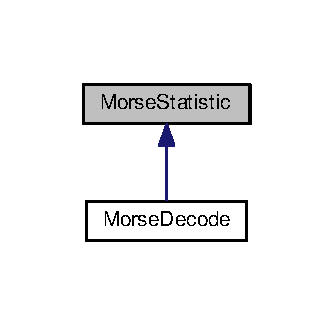
\includegraphics[width=160pt]{classMorseStatistic__inherit__graph}
\end{center}
\end{figure}


Collaboration diagram for Morse\+Statistic\+:\nopagebreak
\begin{figure}[H]
\begin{center}
\leavevmode
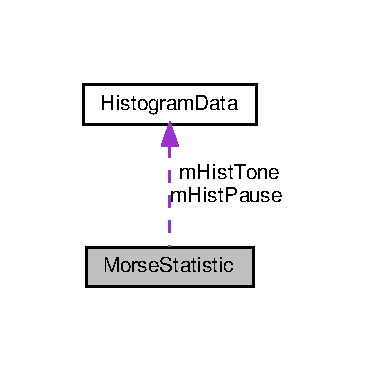
\includegraphics[width=177pt]{classMorseStatistic__coll__graph}
\end{center}
\end{figure}
\subsection*{Public Member Functions}
\begin{DoxyCompactItemize}
\item 
\hyperlink{classMorseStatistic_a48a3dc7e8f56e32caa91689593b07cff}{Morse\+Statistic} ()
\begin{DoxyCompactList}\small\item\em constructor that initialize the buffer \end{DoxyCompactList}\item 
virtual \hyperlink{classMorseStatistic_a9eb933dcacfbc2e124208f901faba46d}{$\sim$\+Morse\+Statistic} ()
\begin{DoxyCompactList}\small\item\em destructor that deletes the buffer \end{DoxyCompactList}\item 
void \hyperlink{classMorseStatistic_ae5f4ab08849cd2cb724748108309661e}{Stat\+Set\+Buffer\+Size} (int buffer\+Size)
\begin{DoxyCompactList}\small\item\em delete buffer and create a new one with the desired size \end{DoxyCompactList}\item 
double \hyperlink{classMorseStatistic_a3347edf33028378ec2009a67c7f5b14d}{Stat\+Get\+Average\+Time} (Morse\+::\+Morse\+Sign sign)
\begin{DoxyCompactList}\small\item\em averages the duration for a morse sign \end{DoxyCompactList}\item 
double \hyperlink{classMorseStatistic_af92781be60bdd00871dcb5907939dcb6}{Stat\+Get\+Std\+Dev\+Of\+Time} (Morse\+::\+Morse\+Sign sign)
\begin{DoxyCompactList}\small\item\em standard deviation for a morse sign \end{DoxyCompactList}\item 
int \hyperlink{classMorseStatistic_a541c0f03283b2327051bb30e2241753a}{Stat\+Get\+Count} (Morse\+::\+Morse\+Sign sign)
\begin{DoxyCompactList}\small\item\em counts the amount of durations for a sign stored in the buffer \end{DoxyCompactList}\item 
int \hyperlink{classMorseStatistic_a92064ea196420fa75a5950a8bdab874e}{Stat\+Edge\+Event\+Buffer\+Full\+Counter} ()
\begin{DoxyCompactList}\small\item\em returns the edge event buffer full counter \end{DoxyCompactList}\item 
void \hyperlink{classMorseStatistic_addefc50d54ca28297ad4ebb50488601d}{Add\+Period\+To\+Histogram} (double period, Morse\+::\+Edge\+State state)
\begin{DoxyCompactList}\small\item\em add period to the tone/pause length histogram \end{DoxyCompactList}\item 
void \hyperlink{classMorseStatistic_a6ba988ce121e1f99cff841f5db6265f8}{Evaluate\+Tone\+In\+Histogram} (bool care)
\begin{DoxyCompactList}\small\item\em switch evaluation of tone period on/off \end{DoxyCompactList}\item 
void \hyperlink{classMorseStatistic_aabfa04ea2d9664fd2d2434698243bbae}{Evaluate\+Pause\+In\+Histogram} (bool care)
\begin{DoxyCompactList}\small\item\em switch evaluation of pause period on/off \end{DoxyCompactList}\item 
bool \hyperlink{classMorseStatistic_ad2f9a6c81583599830803c8024abc507}{Is\+Tone\+Evaluated\+In\+Histogram} ()
\item 
bool \hyperlink{classMorseStatistic_a79840d18d8976b85931f150df0a94e11}{Is\+Pause\+Evaluated\+In\+Histogram} ()
\item 
unsigned short \hyperlink{classMorseStatistic_a7f74b33235ac1c347aa35c778914ca91}{Get\+Number\+Of\+Bins} ()
\begin{DoxyCompactList}\small\item\em return the number of histogram bins \end{DoxyCompactList}\item 
double \hyperlink{classMorseStatistic_a4e421283bff64677db975e258f5c26d6}{Get\+Max\+Period} ()
\begin{DoxyCompactList}\small\item\em largest period that is currently in the histogram \end{DoxyCompactList}\item 
unsigned short \hyperlink{classMorseStatistic_a3467fc7a0aac07feeb1d47805dd603cf}{Get\+Hist\+Tone\+Bin\+Count} (unsigned short bin)
\begin{DoxyCompactList}\small\item\em count the periods that belongs to tones and in a histogram bin. \end{DoxyCompactList}\item 
unsigned short \hyperlink{classMorseStatistic_a4e8fd6695aa502fa339d6a65efb297a7}{Get\+Hist\+Pause\+Bin\+Count} (unsigned short bin)
\begin{DoxyCompactList}\small\item\em count the periods that belongs to pause and in a histogram bin. \end{DoxyCompactList}\end{DoxyCompactItemize}
\subsection*{Protected Member Functions}
\begin{DoxyCompactItemize}
\item 
void \hyperlink{classMorseStatistic_afc0c1198ba34c154ce613591861a339b}{Stat\+Add\+Sample} (Morse\+::\+Morse\+Sign sign, double dt)
\begin{DoxyCompactList}\small\item\em add a sample to the buffer \end{DoxyCompactList}\item 
\mbox{\Hypertarget{classMorseStatistic_a9caf4881a3a6843aa0aafd1aeaee14e2}\label{classMorseStatistic_a9caf4881a3a6843aa0aafd1aeaee14e2}} 
void \hyperlink{classMorseStatistic_a9caf4881a3a6843aa0aafd1aeaee14e2}{Stat\+Edge\+Event\+Buffer\+Full} ()
\begin{DoxyCompactList}\small\item\em increase the edge event buffer full counter \end{DoxyCompactList}\end{DoxyCompactItemize}
\subsection*{Private Member Functions}
\begin{DoxyCompactItemize}
\item 
\mbox{\Hypertarget{classMorseStatistic_a512955d403a9906f15d550e3f731d810}\label{classMorseStatistic_a512955d403a9906f15d550e3f731d810}} 
void \hyperlink{classMorseStatistic_a512955d403a9906f15d550e3f731d810}{Delete\+Buffer} ()
\begin{DoxyCompactList}\small\item\em free the memory used as buffer \end{DoxyCompactList}\item 
void \hyperlink{classMorseStatistic_adc79128f3c472bef513ce8546c833834}{Init\+Buffer} (int buffer\+Size)
\begin{DoxyCompactList}\small\item\em allocate memory for the buffer and initialze it \end{DoxyCompactList}\end{DoxyCompactItemize}
\subsection*{Private Attributes}
\begin{DoxyCompactItemize}
\item 
\mbox{\Hypertarget{classMorseStatistic_ac778af78c64cc2a700e09dc78dc300a7}\label{classMorseStatistic_ac778af78c64cc2a700e09dc78dc300a7}} 
Morse\+::\+Morse\+Sign $\ast$ \hyperlink{classMorseStatistic_ac778af78c64cc2a700e09dc78dc300a7}{m\+Morse\+Sign\+Buffer}
\begin{DoxyCompactList}\small\item\em buffer to store last morse signs \end{DoxyCompactList}\item 
\mbox{\Hypertarget{classMorseStatistic_a376ed110e487f81bf51547e28c366d34}\label{classMorseStatistic_a376ed110e487f81bf51547e28c366d34}} 
double $\ast$ \hyperlink{classMorseStatistic_a376ed110e487f81bf51547e28c366d34}{m\+Morse\+Time\+Buffer}
\begin{DoxyCompactList}\small\item\em buffer to store duration of the morse signs \end{DoxyCompactList}\item 
\mbox{\Hypertarget{classMorseStatistic_a1c05e54ba3bbdf68153cba828bfc019f}\label{classMorseStatistic_a1c05e54ba3bbdf68153cba828bfc019f}} 
int \hyperlink{classMorseStatistic_a1c05e54ba3bbdf68153cba828bfc019f}{m\+Buffer\+Size}
\begin{DoxyCompactList}\small\item\em size of the buffers \end{DoxyCompactList}\item 
\mbox{\Hypertarget{classMorseStatistic_acf145c45629cca3568ec7d69c94ccce2}\label{classMorseStatistic_acf145c45629cca3568ec7d69c94ccce2}} 
int \hyperlink{classMorseStatistic_acf145c45629cca3568ec7d69c94ccce2}{m\+Buffer\+Index}
\begin{DoxyCompactList}\small\item\em index of the buffer element that will be written next \end{DoxyCompactList}\item 
\mbox{\Hypertarget{classMorseStatistic_a60c80a05c589975e44063a02bbf9b933}\label{classMorseStatistic_a60c80a05c589975e44063a02bbf9b933}} 
int \hyperlink{classMorseStatistic_a60c80a05c589975e44063a02bbf9b933}{m\+Edge\+Event\+Buffer\+Full\+Counter}
\begin{DoxyCompactList}\small\item\em counts how often the edge event buffer overflowed \end{DoxyCompactList}\item 
\mbox{\Hypertarget{classMorseStatistic_ad6d750d1fc27d717848c5521e190c285}\label{classMorseStatistic_ad6d750d1fc27d717848c5521e190c285}} 
\hyperlink{classHistogramData}{Histogram\+Data} \hyperlink{classMorseStatistic_ad6d750d1fc27d717848c5521e190c285}{m\+Hist\+Tone}
\begin{DoxyCompactList}\small\item\em instance of the histogram data class containing the tone histogram \end{DoxyCompactList}\item 
\mbox{\Hypertarget{classMorseStatistic_a44400e85e42ddd4e273ba259a293f6b2}\label{classMorseStatistic_a44400e85e42ddd4e273ba259a293f6b2}} 
\hyperlink{classHistogramData}{Histogram\+Data} \hyperlink{classMorseStatistic_a44400e85e42ddd4e273ba259a293f6b2}{m\+Hist\+Pause}
\begin{DoxyCompactList}\small\item\em instance of the histogram data class containing the pause histogram \end{DoxyCompactList}\end{DoxyCompactItemize}


\subsection{Detailed Description}
The morse statistic class collects data from the decode process. 

\begin{DoxyAuthor}{Author}
Matthias Hund 
\end{DoxyAuthor}
\begin{DoxyDate}{Date}
05/25/20 
\end{DoxyDate}


\subsection{Constructor \& Destructor Documentation}
\mbox{\Hypertarget{classMorseStatistic_a48a3dc7e8f56e32caa91689593b07cff}\label{classMorseStatistic_a48a3dc7e8f56e32caa91689593b07cff}} 
\index{Morse\+Statistic@{Morse\+Statistic}!Morse\+Statistic@{Morse\+Statistic}}
\index{Morse\+Statistic@{Morse\+Statistic}!Morse\+Statistic@{Morse\+Statistic}}
\subsubsection{\texorpdfstring{Morse\+Statistic()}{MorseStatistic()}}
{\footnotesize\ttfamily Morse\+Statistic\+::\+Morse\+Statistic (\begin{DoxyParamCaption}{ }\end{DoxyParamCaption})}



constructor that initialize the buffer 

\begin{DoxyReturn}{Returns}

\end{DoxyReturn}
\mbox{\Hypertarget{classMorseStatistic_a9eb933dcacfbc2e124208f901faba46d}\label{classMorseStatistic_a9eb933dcacfbc2e124208f901faba46d}} 
\index{Morse\+Statistic@{Morse\+Statistic}!````~Morse\+Statistic@{$\sim$\+Morse\+Statistic}}
\index{````~Morse\+Statistic@{$\sim$\+Morse\+Statistic}!Morse\+Statistic@{Morse\+Statistic}}
\subsubsection{\texorpdfstring{$\sim$\+Morse\+Statistic()}{~MorseStatistic()}}
{\footnotesize\ttfamily Morse\+Statistic\+::$\sim$\+Morse\+Statistic (\begin{DoxyParamCaption}{ }\end{DoxyParamCaption})\hspace{0.3cm}{\ttfamily [virtual]}}



destructor that deletes the buffer 

\begin{DoxyReturn}{Returns}

\end{DoxyReturn}


\subsection{Member Function Documentation}
\mbox{\Hypertarget{classMorseStatistic_addefc50d54ca28297ad4ebb50488601d}\label{classMorseStatistic_addefc50d54ca28297ad4ebb50488601d}} 
\index{Morse\+Statistic@{Morse\+Statistic}!Add\+Period\+To\+Histogram@{Add\+Period\+To\+Histogram}}
\index{Add\+Period\+To\+Histogram@{Add\+Period\+To\+Histogram}!Morse\+Statistic@{Morse\+Statistic}}
\subsubsection{\texorpdfstring{Add\+Period\+To\+Histogram()}{AddPeriodToHistogram()}}
{\footnotesize\ttfamily void Morse\+Statistic\+::\+Add\+Period\+To\+Histogram (\begin{DoxyParamCaption}\item[{double}]{period,  }\item[{Morse\+::\+Edge\+State}]{state }\end{DoxyParamCaption})}



add period to the tone/pause length histogram 


\begin{DoxyParams}{Parameters}
{\em period} & period of the tone or pause in seconds \\
\hline
{\em state} & F\+A\+L\+L\+I\+NG if period belongs to a tone or R\+I\+S\+I\+NG if period belongs to a pause \\
\hline
\end{DoxyParams}
\mbox{\Hypertarget{classMorseStatistic_aabfa04ea2d9664fd2d2434698243bbae}\label{classMorseStatistic_aabfa04ea2d9664fd2d2434698243bbae}} 
\index{Morse\+Statistic@{Morse\+Statistic}!Evaluate\+Pause\+In\+Histogram@{Evaluate\+Pause\+In\+Histogram}}
\index{Evaluate\+Pause\+In\+Histogram@{Evaluate\+Pause\+In\+Histogram}!Morse\+Statistic@{Morse\+Statistic}}
\subsubsection{\texorpdfstring{Evaluate\+Pause\+In\+Histogram()}{EvaluatePauseInHistogram()}}
{\footnotesize\ttfamily void Morse\+Statistic\+::\+Evaluate\+Pause\+In\+Histogram (\begin{DoxyParamCaption}\item[{bool}]{care }\end{DoxyParamCaption})}



switch evaluation of pause period on/off 


\begin{DoxyParams}{Parameters}
{\em care} & if true all periods that belong to a pause are evaluated in the histogram, otherwise periods are filtered out \\
\hline
\end{DoxyParams}
\mbox{\Hypertarget{classMorseStatistic_a6ba988ce121e1f99cff841f5db6265f8}\label{classMorseStatistic_a6ba988ce121e1f99cff841f5db6265f8}} 
\index{Morse\+Statistic@{Morse\+Statistic}!Evaluate\+Tone\+In\+Histogram@{Evaluate\+Tone\+In\+Histogram}}
\index{Evaluate\+Tone\+In\+Histogram@{Evaluate\+Tone\+In\+Histogram}!Morse\+Statistic@{Morse\+Statistic}}
\subsubsection{\texorpdfstring{Evaluate\+Tone\+In\+Histogram()}{EvaluateToneInHistogram()}}
{\footnotesize\ttfamily void Morse\+Statistic\+::\+Evaluate\+Tone\+In\+Histogram (\begin{DoxyParamCaption}\item[{bool}]{care }\end{DoxyParamCaption})}



switch evaluation of tone period on/off 


\begin{DoxyParams}{Parameters}
{\em care} & if true all periods that belong to a tone are evaluated in the histogram, otherwise periods are filtered out \\
\hline
\end{DoxyParams}
\mbox{\Hypertarget{classMorseStatistic_a4e8fd6695aa502fa339d6a65efb297a7}\label{classMorseStatistic_a4e8fd6695aa502fa339d6a65efb297a7}} 
\index{Morse\+Statistic@{Morse\+Statistic}!Get\+Hist\+Pause\+Bin\+Count@{Get\+Hist\+Pause\+Bin\+Count}}
\index{Get\+Hist\+Pause\+Bin\+Count@{Get\+Hist\+Pause\+Bin\+Count}!Morse\+Statistic@{Morse\+Statistic}}
\subsubsection{\texorpdfstring{Get\+Hist\+Pause\+Bin\+Count()}{GetHistPauseBinCount()}}
{\footnotesize\ttfamily unsigned short Morse\+Statistic\+::\+Get\+Hist\+Pause\+Bin\+Count (\begin{DoxyParamCaption}\item[{unsigned short}]{bin }\end{DoxyParamCaption})}



count the periods that belongs to pause and in a histogram bin. 


\begin{DoxyParams}{Parameters}
{\em bin} & number of the histogram bin \\
\hline
\end{DoxyParams}
\begin{DoxyReturn}{Returns}
return the number of periods that are element of the range regarding to the historam bin 
\end{DoxyReturn}
\mbox{\Hypertarget{classMorseStatistic_a3467fc7a0aac07feeb1d47805dd603cf}\label{classMorseStatistic_a3467fc7a0aac07feeb1d47805dd603cf}} 
\index{Morse\+Statistic@{Morse\+Statistic}!Get\+Hist\+Tone\+Bin\+Count@{Get\+Hist\+Tone\+Bin\+Count}}
\index{Get\+Hist\+Tone\+Bin\+Count@{Get\+Hist\+Tone\+Bin\+Count}!Morse\+Statistic@{Morse\+Statistic}}
\subsubsection{\texorpdfstring{Get\+Hist\+Tone\+Bin\+Count()}{GetHistToneBinCount()}}
{\footnotesize\ttfamily unsigned short Morse\+Statistic\+::\+Get\+Hist\+Tone\+Bin\+Count (\begin{DoxyParamCaption}\item[{unsigned short}]{bin }\end{DoxyParamCaption})}



count the periods that belongs to tones and in a histogram bin. 


\begin{DoxyParams}{Parameters}
{\em bin} & number of the histogram bin \\
\hline
\end{DoxyParams}
\begin{DoxyReturn}{Returns}
return the number of periods that are element of the range regarding to the historam bin 
\end{DoxyReturn}
\mbox{\Hypertarget{classMorseStatistic_a4e421283bff64677db975e258f5c26d6}\label{classMorseStatistic_a4e421283bff64677db975e258f5c26d6}} 
\index{Morse\+Statistic@{Morse\+Statistic}!Get\+Max\+Period@{Get\+Max\+Period}}
\index{Get\+Max\+Period@{Get\+Max\+Period}!Morse\+Statistic@{Morse\+Statistic}}
\subsubsection{\texorpdfstring{Get\+Max\+Period()}{GetMaxPeriod()}}
{\footnotesize\ttfamily double Morse\+Statistic\+::\+Get\+Max\+Period (\begin{DoxyParamCaption}{ }\end{DoxyParamCaption})}



largest period that is currently in the histogram 

\begin{DoxyReturn}{Returns}
period in seconds 
\end{DoxyReturn}
\mbox{\Hypertarget{classMorseStatistic_a7f74b33235ac1c347aa35c778914ca91}\label{classMorseStatistic_a7f74b33235ac1c347aa35c778914ca91}} 
\index{Morse\+Statistic@{Morse\+Statistic}!Get\+Number\+Of\+Bins@{Get\+Number\+Of\+Bins}}
\index{Get\+Number\+Of\+Bins@{Get\+Number\+Of\+Bins}!Morse\+Statistic@{Morse\+Statistic}}
\subsubsection{\texorpdfstring{Get\+Number\+Of\+Bins()}{GetNumberOfBins()}}
{\footnotesize\ttfamily unsigned short Morse\+Statistic\+::\+Get\+Number\+Of\+Bins (\begin{DoxyParamCaption}{ }\end{DoxyParamCaption})}



return the number of histogram bins 

\begin{DoxyReturn}{Returns}
the number of bins 
\end{DoxyReturn}
\mbox{\Hypertarget{classMorseStatistic_adc79128f3c472bef513ce8546c833834}\label{classMorseStatistic_adc79128f3c472bef513ce8546c833834}} 
\index{Morse\+Statistic@{Morse\+Statistic}!Init\+Buffer@{Init\+Buffer}}
\index{Init\+Buffer@{Init\+Buffer}!Morse\+Statistic@{Morse\+Statistic}}
\subsubsection{\texorpdfstring{Init\+Buffer()}{InitBuffer()}}
{\footnotesize\ttfamily void Morse\+Statistic\+::\+Init\+Buffer (\begin{DoxyParamCaption}\item[{int}]{buffer\+Size }\end{DoxyParamCaption})\hspace{0.3cm}{\ttfamily [private]}}



allocate memory for the buffer and initialze it 


\begin{DoxyParams}{Parameters}
{\em buffer\+Size} & \\
\hline
\end{DoxyParams}
\mbox{\Hypertarget{classMorseStatistic_a79840d18d8976b85931f150df0a94e11}\label{classMorseStatistic_a79840d18d8976b85931f150df0a94e11}} 
\index{Morse\+Statistic@{Morse\+Statistic}!Is\+Pause\+Evaluated\+In\+Histogram@{Is\+Pause\+Evaluated\+In\+Histogram}}
\index{Is\+Pause\+Evaluated\+In\+Histogram@{Is\+Pause\+Evaluated\+In\+Histogram}!Morse\+Statistic@{Morse\+Statistic}}
\subsubsection{\texorpdfstring{Is\+Pause\+Evaluated\+In\+Histogram()}{IsPauseEvaluatedInHistogram()}}
{\footnotesize\ttfamily bool Morse\+Statistic\+::\+Is\+Pause\+Evaluated\+In\+Histogram (\begin{DoxyParamCaption}{ }\end{DoxyParamCaption})}

\begin{DoxyReturn}{Returns}
return true if periods of pauses are evaluated in the histogram, otherwise the function return false 
\end{DoxyReturn}
\mbox{\Hypertarget{classMorseStatistic_ad2f9a6c81583599830803c8024abc507}\label{classMorseStatistic_ad2f9a6c81583599830803c8024abc507}} 
\index{Morse\+Statistic@{Morse\+Statistic}!Is\+Tone\+Evaluated\+In\+Histogram@{Is\+Tone\+Evaluated\+In\+Histogram}}
\index{Is\+Tone\+Evaluated\+In\+Histogram@{Is\+Tone\+Evaluated\+In\+Histogram}!Morse\+Statistic@{Morse\+Statistic}}
\subsubsection{\texorpdfstring{Is\+Tone\+Evaluated\+In\+Histogram()}{IsToneEvaluatedInHistogram()}}
{\footnotesize\ttfamily bool Morse\+Statistic\+::\+Is\+Tone\+Evaluated\+In\+Histogram (\begin{DoxyParamCaption}{ }\end{DoxyParamCaption})}

\begin{DoxyReturn}{Returns}
return true if periods of tones are evaluated in the histogram, otherwise the function return false 
\end{DoxyReturn}
\mbox{\Hypertarget{classMorseStatistic_afc0c1198ba34c154ce613591861a339b}\label{classMorseStatistic_afc0c1198ba34c154ce613591861a339b}} 
\index{Morse\+Statistic@{Morse\+Statistic}!Stat\+Add\+Sample@{Stat\+Add\+Sample}}
\index{Stat\+Add\+Sample@{Stat\+Add\+Sample}!Morse\+Statistic@{Morse\+Statistic}}
\subsubsection{\texorpdfstring{Stat\+Add\+Sample()}{StatAddSample()}}
{\footnotesize\ttfamily void Morse\+Statistic\+::\+Stat\+Add\+Sample (\begin{DoxyParamCaption}\item[{Morse\+::\+Morse\+Sign}]{sign,  }\item[{double}]{dt }\end{DoxyParamCaption})\hspace{0.3cm}{\ttfamily [protected]}}



add a sample to the buffer 


\begin{DoxyParams}{Parameters}
{\em sign} & morse sign that is added \\
\hline
{\em dt} & duration that is addef \\
\hline
\end{DoxyParams}
\mbox{\Hypertarget{classMorseStatistic_a92064ea196420fa75a5950a8bdab874e}\label{classMorseStatistic_a92064ea196420fa75a5950a8bdab874e}} 
\index{Morse\+Statistic@{Morse\+Statistic}!Stat\+Edge\+Event\+Buffer\+Full\+Counter@{Stat\+Edge\+Event\+Buffer\+Full\+Counter}}
\index{Stat\+Edge\+Event\+Buffer\+Full\+Counter@{Stat\+Edge\+Event\+Buffer\+Full\+Counter}!Morse\+Statistic@{Morse\+Statistic}}
\subsubsection{\texorpdfstring{Stat\+Edge\+Event\+Buffer\+Full\+Counter()}{StatEdgeEventBufferFullCounter()}}
{\footnotesize\ttfamily int Morse\+Statistic\+::\+Stat\+Edge\+Event\+Buffer\+Full\+Counter (\begin{DoxyParamCaption}{ }\end{DoxyParamCaption})}



returns the edge event buffer full counter 

\begin{DoxyReturn}{Returns}
edge event buffer full counter 
\end{DoxyReturn}
\mbox{\Hypertarget{classMorseStatistic_a3347edf33028378ec2009a67c7f5b14d}\label{classMorseStatistic_a3347edf33028378ec2009a67c7f5b14d}} 
\index{Morse\+Statistic@{Morse\+Statistic}!Stat\+Get\+Average\+Time@{Stat\+Get\+Average\+Time}}
\index{Stat\+Get\+Average\+Time@{Stat\+Get\+Average\+Time}!Morse\+Statistic@{Morse\+Statistic}}
\subsubsection{\texorpdfstring{Stat\+Get\+Average\+Time()}{StatGetAverageTime()}}
{\footnotesize\ttfamily double Morse\+Statistic\+::\+Stat\+Get\+Average\+Time (\begin{DoxyParamCaption}\item[{Morse\+::\+Morse\+Sign}]{sign }\end{DoxyParamCaption})}



averages the duration for a morse sign 


\begin{DoxyParams}{Parameters}
{\em sign} & morse sign for which the average is calculated \\
\hline
\end{DoxyParams}
\begin{DoxyReturn}{Returns}
the average duration in seconds of the sign 
\end{DoxyReturn}
\mbox{\Hypertarget{classMorseStatistic_a541c0f03283b2327051bb30e2241753a}\label{classMorseStatistic_a541c0f03283b2327051bb30e2241753a}} 
\index{Morse\+Statistic@{Morse\+Statistic}!Stat\+Get\+Count@{Stat\+Get\+Count}}
\index{Stat\+Get\+Count@{Stat\+Get\+Count}!Morse\+Statistic@{Morse\+Statistic}}
\subsubsection{\texorpdfstring{Stat\+Get\+Count()}{StatGetCount()}}
{\footnotesize\ttfamily int Morse\+Statistic\+::\+Stat\+Get\+Count (\begin{DoxyParamCaption}\item[{Morse\+::\+Morse\+Sign}]{sign }\end{DoxyParamCaption})}



counts the amount of durations for a sign stored in the buffer 


\begin{DoxyParams}{Parameters}
{\em sign} & morse sign \\
\hline
\end{DoxyParams}
\begin{DoxyReturn}{Returns}
durations stored in the buffer 
\end{DoxyReturn}
\mbox{\Hypertarget{classMorseStatistic_af92781be60bdd00871dcb5907939dcb6}\label{classMorseStatistic_af92781be60bdd00871dcb5907939dcb6}} 
\index{Morse\+Statistic@{Morse\+Statistic}!Stat\+Get\+Std\+Dev\+Of\+Time@{Stat\+Get\+Std\+Dev\+Of\+Time}}
\index{Stat\+Get\+Std\+Dev\+Of\+Time@{Stat\+Get\+Std\+Dev\+Of\+Time}!Morse\+Statistic@{Morse\+Statistic}}
\subsubsection{\texorpdfstring{Stat\+Get\+Std\+Dev\+Of\+Time()}{StatGetStdDevOfTime()}}
{\footnotesize\ttfamily double Morse\+Statistic\+::\+Stat\+Get\+Std\+Dev\+Of\+Time (\begin{DoxyParamCaption}\item[{Morse\+::\+Morse\+Sign}]{sign }\end{DoxyParamCaption})}



standard deviation for a morse sign 


\begin{DoxyParams}{Parameters}
{\em sign} & morse sign for which the standard deviation is calculated \\
\hline
\end{DoxyParams}
\begin{DoxyReturn}{Returns}
the standard deviation of the sign 
\end{DoxyReturn}
\mbox{\Hypertarget{classMorseStatistic_ae5f4ab08849cd2cb724748108309661e}\label{classMorseStatistic_ae5f4ab08849cd2cb724748108309661e}} 
\index{Morse\+Statistic@{Morse\+Statistic}!Stat\+Set\+Buffer\+Size@{Stat\+Set\+Buffer\+Size}}
\index{Stat\+Set\+Buffer\+Size@{Stat\+Set\+Buffer\+Size}!Morse\+Statistic@{Morse\+Statistic}}
\subsubsection{\texorpdfstring{Stat\+Set\+Buffer\+Size()}{StatSetBufferSize()}}
{\footnotesize\ttfamily void Morse\+Statistic\+::\+Stat\+Set\+Buffer\+Size (\begin{DoxyParamCaption}\item[{int}]{buffer\+Size }\end{DoxyParamCaption})}



delete buffer and create a new one with the desired size 


\begin{DoxyParams}{Parameters}
{\em buffer\+Size} & size of the new buffer \\
\hline
\end{DoxyParams}


The documentation for this class was generated from the following files\+:\begin{DoxyCompactItemize}
\item 
\hyperlink{MorseStatistic_8h}{Morse\+Statistic.\+h}\item 
Morse\+Statistic.\+cpp\end{DoxyCompactItemize}

\chapter{File Documentation}
\hypertarget{ConfigFile_8h}{}\section{Config\+File.\+h File Reference}
\label{ConfigFile_8h}\index{Config\+File.\+h@{Config\+File.\+h}}


Reads configuration from a file. Each line of the file should consist a empty, a comment or ar parameter name/value pair.  


{\ttfamily \#include $<$fstream$>$}\newline
{\ttfamily \#include $<$list$>$}\newline
{\ttfamily \#include $<$string$>$}\newline
{\ttfamily \#include $<$tuple$>$}\newline
Include dependency graph for Config\+File.\+h\+:\nopagebreak
\begin{figure}[H]
\begin{center}
\leavevmode
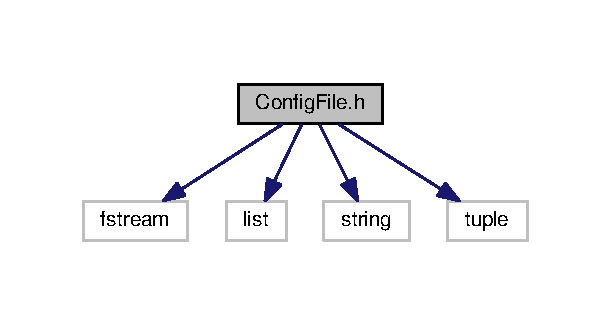
\includegraphics[width=293pt]{ConfigFile_8h__incl}
\end{center}
\end{figure}
This graph shows which files directly or indirectly include this file\+:\nopagebreak
\begin{figure}[H]
\begin{center}
\leavevmode
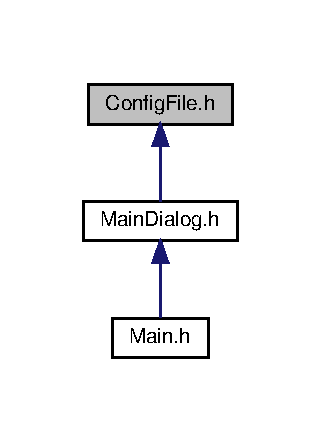
\includegraphics[width=154pt]{ConfigFile_8h__dep__incl}
\end{center}
\end{figure}
\subsection*{Classes}
\begin{DoxyCompactItemize}
\item 
class \hyperlink{classConfigFile}{Config\+File}
\end{DoxyCompactItemize}


\subsection{Detailed Description}
Reads configuration from a file. Each line of the file should consist a empty, a comment or ar parameter name/value pair. 


\hypertarget{Global_8h}{}\section{Global.\+h File Reference}
\label{Global_8h}\index{Global.\+h@{Global.\+h}}


container for data that is accessed from different threads  


{\ttfamily \#include \char`\"{}Morse\+Decode.\+h\char`\"{}}\newline
{\ttfamily \#include $<$mutex$>$}\newline
Include dependency graph for Global.\+h\+:
\nopagebreak
\begin{figure}[H]
\begin{center}
\leavevmode
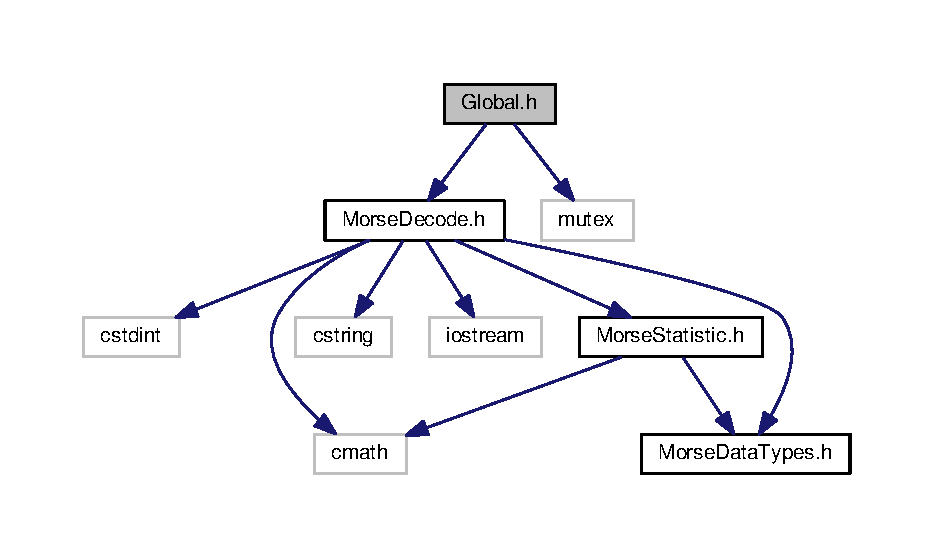
\includegraphics[width=350pt]{Global_8h__incl}
\end{center}
\end{figure}
\subsection*{Classes}
\begin{DoxyCompactItemize}
\item 
class \hyperlink{classGlobal}{Global}
\end{DoxyCompactItemize}


\subsection{Detailed Description}
container for data that is accessed from different threads 


\hypertarget{Main_8h}{}\section{Main.\+h File Reference}
\label{Main_8h}\index{Main.\+h@{Main.\+h}}


application class declaration  


{\ttfamily \#include $<$wx/wx.\+h$>$}\newline
{\ttfamily \#include \char`\"{}Main\+Dialog.\+h\char`\"{}}\newline
Include dependency graph for Main.\+h\+:
\nopagebreak
\begin{figure}[H]
\begin{center}
\leavevmode
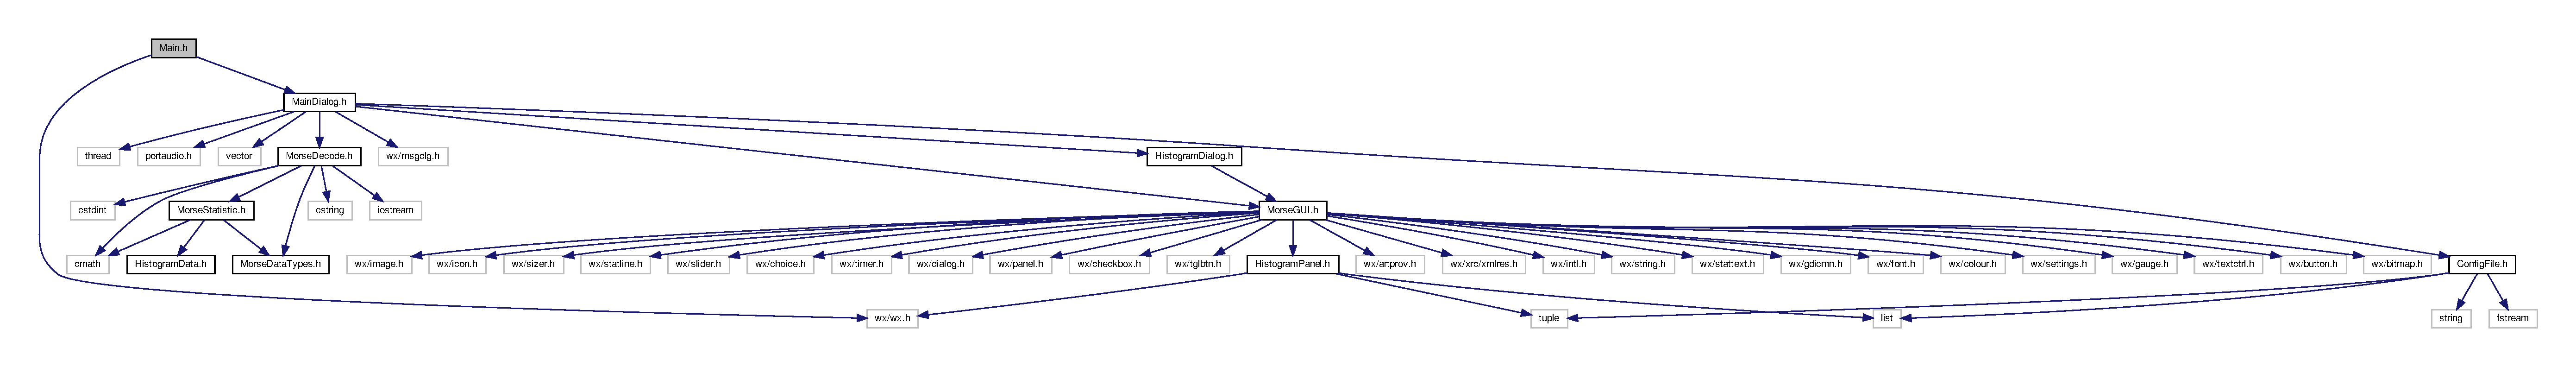
\includegraphics[width=350pt]{Main_8h__incl}
\end{center}
\end{figure}
\subsection*{Classes}
\begin{DoxyCompactItemize}
\item 
class \hyperlink{classMainApp}{Main\+App}
\end{DoxyCompactItemize}


\subsection{Detailed Description}
application class declaration 


\hypertarget{MainDialog_8h}{}\section{Main\+Dialog.\+h File Reference}
\label{MainDialog_8h}\index{Main\+Dialog.\+h@{Main\+Dialog.\+h}}


subclass of the wx\+Form\+Builder generated \hyperlink{classMainDialogBase}{Main\+Dialog\+Base} that inherit the elements of the gui and add some functionality to it  


{\ttfamily \#include $<$thread$>$}\newline
{\ttfamily \#include $<$portaudio.\+h$>$}\newline
{\ttfamily \#include $<$vector$>$}\newline
{\ttfamily \#include \char`\"{}Morse\+G\+U\+I.\+h\char`\"{}}\newline
{\ttfamily \#include \char`\"{}Morse\+Decode.\+h\char`\"{}}\newline
{\ttfamily \#include \char`\"{}Config\+File.\+h\char`\"{}}\newline
{\ttfamily \#include $<$wx/msgdlg.\+h$>$}\newline
Include dependency graph for Main\+Dialog.\+h\+:\nopagebreak
\begin{figure}[H]
\begin{center}
\leavevmode
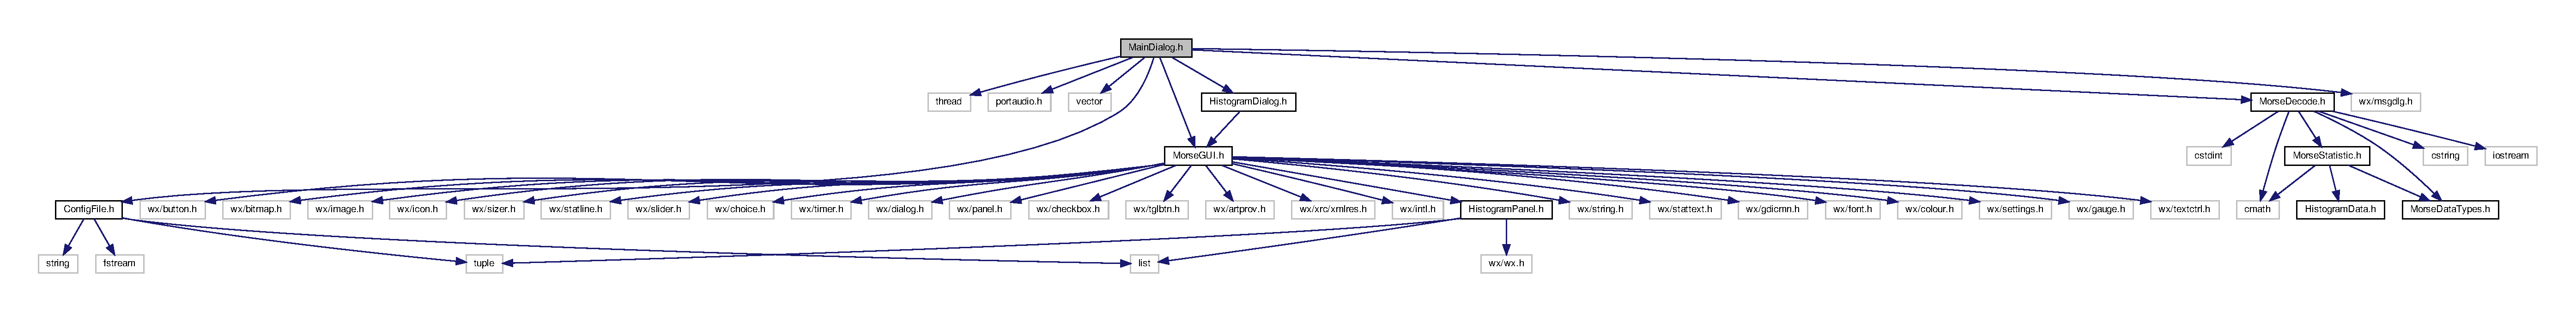
\includegraphics[width=350pt]{MainDialog_8h__incl}
\end{center}
\end{figure}
This graph shows which files directly or indirectly include this file\+:\nopagebreak
\begin{figure}[H]
\begin{center}
\leavevmode
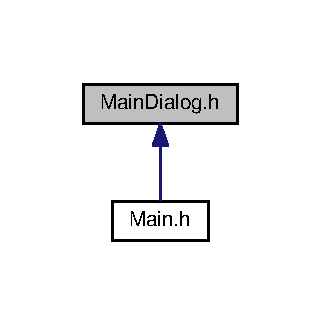
\includegraphics[width=154pt]{MainDialog_8h__dep__incl}
\end{center}
\end{figure}
\subsection*{Classes}
\begin{DoxyCompactItemize}
\item 
class \hyperlink{classMainDialog}{Main\+Dialog}
\end{DoxyCompactItemize}


\subsection{Detailed Description}
subclass of the wx\+Form\+Builder generated \hyperlink{classMainDialogBase}{Main\+Dialog\+Base} that inherit the elements of the gui and add some functionality to it 

Subclass of \hyperlink{classMainDialogBase}{Main\+Dialog\+Base}, which is generated by wx\+Form\+Builder.
\hypertarget{MorseDecode_8h}{}\section{Morse\+Decode.\+h File Reference}
\label{MorseDecode_8h}\index{Morse\+Decode.\+h@{Morse\+Decode.\+h}}
{\ttfamily \#include $<$cstdint$>$}\newline
{\ttfamily \#include $<$cmath$>$}\newline
{\ttfamily \#include $<$cstring$>$}\newline
{\ttfamily \#include $<$iostream$>$}\newline
{\ttfamily \#include \char`\"{}Morse\+Data\+Types.\+h\char`\"{}}\newline
{\ttfamily \#include \char`\"{}Morse\+Statistic.\+h\char`\"{}}\newline
Include dependency graph for Morse\+Decode.\+h\+:\nopagebreak
\begin{figure}[H]
\begin{center}
\leavevmode
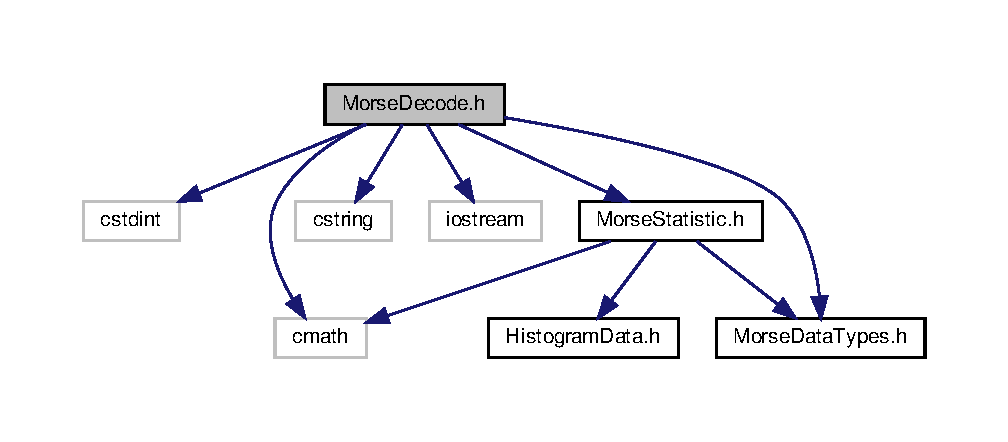
\includegraphics[width=350pt]{MorseDecode_8h__incl}
\end{center}
\end{figure}
This graph shows which files directly or indirectly include this file\+:\nopagebreak
\begin{figure}[H]
\begin{center}
\leavevmode
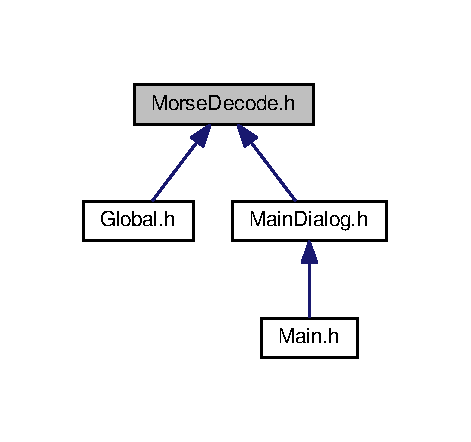
\includegraphics[width=226pt]{MorseDecode_8h__dep__incl}
\end{center}
\end{figure}
\subsection*{Classes}
\begin{DoxyCompactItemize}
\item 
class \hyperlink{classMorseDecode}{Morse\+Decode}
\begin{DoxyCompactList}\small\item\em The morse decoder class process a audio stream and output morse signals as a text. \end{DoxyCompactList}\end{DoxyCompactItemize}

\hypertarget{MorseStatistic_8h}{}\section{Morse\+Statistic.\+h File Reference}
\label{MorseStatistic_8h}\index{Morse\+Statistic.\+h@{Morse\+Statistic.\+h}}
{\ttfamily \#include $<$cmath$>$}\newline
{\ttfamily \#include \char`\"{}Morse\+Data\+Types.\+h\char`\"{}}\newline
Include dependency graph for Morse\+Statistic.\+h\+:\nopagebreak
\begin{figure}[H]
\begin{center}
\leavevmode
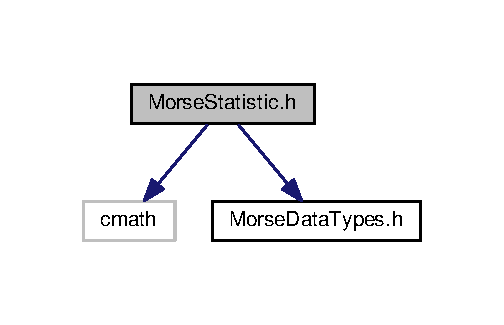
\includegraphics[width=242pt]{MorseStatistic_8h__incl}
\end{center}
\end{figure}
This graph shows which files directly or indirectly include this file\+:\nopagebreak
\begin{figure}[H]
\begin{center}
\leavevmode
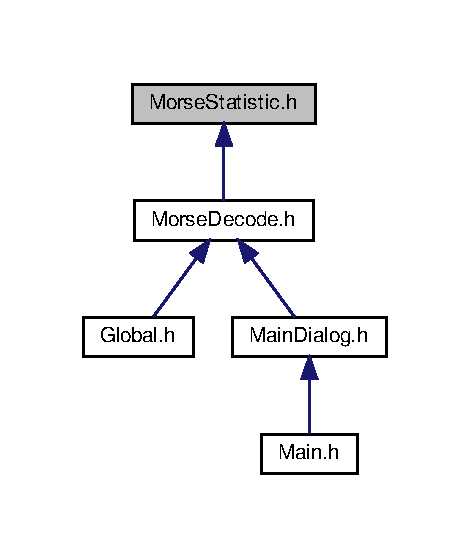
\includegraphics[width=226pt]{MorseStatistic_8h__dep__incl}
\end{center}
\end{figure}
\subsection*{Classes}
\begin{DoxyCompactItemize}
\item 
class \hyperlink{classMorseStatistic}{Morse\+Statistic}
\begin{DoxyCompactList}\small\item\em The morse statistic class collects data from the decode process. \end{DoxyCompactList}\end{DoxyCompactItemize}

%--- End generated contents ---

% Index
\backmatter
\newpage
\phantomsection
\clearemptydoublepage
\addcontentsline{toc}{chapter}{Index}
\printindex

\end{document}
